% Course information source: :contentReference[oaicite:0]{index=0}
\documentclass[12pt]{article}

%==================== PACKAGES ====================
\usepackage[margin=0.9in]{geometry}
\usepackage{amsmath,amssymb,amsthm}
\usepackage{enumitem}
\usepackage{bm}
\usepackage{fancyhdr}
\usepackage{xcolor}
\usepackage{array}
\usepackage{booktabs}
\usepackage{tikz}
\usepackage{pgfplots}
\pgfplotsset{compat=1.17}
\usepackage{tcolorbox}
\tcbuselibrary{theorems,skins,breakable}
\usepackage{graphicx}
\usepackage{multicol}
\usepackage{titlesec}

% MOVE HYPERREF HERE
\usepackage{hyperref} 

\usepackage{draftwatermark}


%==================================================
% COURSE METADATA (EDIT THESE FOR EACH MODULE)
%==================================================
\newcommand{\CourseCode}{MH1101}
\newcommand{\CourseName}{Calculus II}
\newcommand{\DocType}{Revision Notes}
\newcommand{\AcademicYear}{Academic Year 2025--2026}

%==================================================
% TCOLORBOX THEOREM STYLES
%==================================================

% ---------- DEFINITION: dark green, title in darker band ----------
\newtcbtheorem[number within=section]{definition}{Definition}%
{enhanced,
 breakable=false,
 colback=green!5!white,        % light interior
 colframe=green!40!black,      % border
 colbacktitle=green!50!black,  % dark title band
 coltitle=white,               % title text colour
 fonttitle=\bfseries,
 title filled,                 % puts title inside the band
 boxed title style={
   size=small,
   top=2pt, bottom=2pt,
   left=6pt, right=6pt,
   arc=1pt, outer arc=1pt
 },
 boxrule=0.9pt,
 arc=1pt,
 left=8pt, right=8pt, top=10pt, bottom=8pt,
 before skip=12pt, after skip=12pt
}{def}

% ---------- THEOREM: blue, title in darker band ----------
\newtcbtheorem[number within=section]{theorem}{Theorem}%
{enhanced,
 breakable=false,
 colback=blue!3!white,
 colframe=blue!40!black,
 colbacktitle=blue!55!black,
 coltitle=white,
 fonttitle=\bfseries,
 title filled,
 boxed title style={
   size=small,
   top=2pt, bottom=2pt,
   left=6pt, right=6pt,
   arc=1pt, outer arc=1pt
 },
 boxrule=0.9pt,
 arc=1pt,
 left=8pt, right=8pt, top=10pt, bottom=8pt,
 before skip=12pt, after skip=12pt
}{thm}

% ---------- ENVIRONMENTS USING TCOLORBOXENVIRONMENT ----------
\tcolorboxenvironment{identity}{
  enhanced,
  breakable=false,
  colback=green!5!white,
  colframe=green!60!black,
  fonttitle=\bfseries,
  boxrule=1pt,
  arc=3pt,
  left=8pt, right=8pt, top=8pt, bottom=8pt,
  before skip=12pt, after skip=12pt
}

\tcolorboxenvironment{principle}{
  enhanced,
  breakable=false,
  colback=red!5!white,
  colframe=red!60!black,
  fonttitle=\bfseries,
  boxrule=1pt,
  arc=3pt,
  left=8pt, right=8pt, top=8pt, bottom=8pt,
  before skip=12pt, after skip=12pt
}

%==================================================
% CUSTOM TCOLORBOX ENVIRONMENTS (WITH NAMES)
%==================================================
% Optional argument [1][] lets you override the default title if needed:
%   \begin{keyformula}[title={Key Formula: Demand Curve}] ... \end{keyformula}

\newtcolorbox{keyformula}[1][]{
    enhanced,
    breakable=false,
    colback=blue!5!white,
    colframe=blue!75!black,
    title=Key Formula,
    fonttitle=\bfseries,
    boxrule=0.9pt,
    arc=2pt,
    left=8pt, right=8pt, top=8pt, bottom=8pt,
    #1
}

% *** CHANGED TO BROWN AS REQUESTED ***
\newtcolorbox{examplebox}[1][]{
    enhanced,
    breakable=false,
    colback=brown!5!white,
    colframe=brown!75!black,
    title=Worked Example,
    fonttitle=\bfseries,
    boxrule=0.9pt,
    arc=2pt,
    left=8pt, right=8pt, top=8pt, bottom=8pt,
    #1
}

\newtcolorbox{commonmistake}[1][]{
    enhanced,
    breakable=false,
    colback=red!5!white,
    colframe=red!75!black,
    title=Common Mistake,
    fonttitle=\bfseries,
    boxrule=0.9pt,
    arc=2pt,
    left=8pt, right=8pt, top=8pt, bottom=8pt,
    #1
}

\newtcolorbox{policynote}[1][]{
    enhanced,
    breakable=false,
    colback=yellow!10!white,
    colframe=orange!75!black,
    title=Policy Application,
    fonttitle=\bfseries,
    boxrule=0.9pt,
    arc=2pt,
    left=8pt, right=8pt, top=8pt, bottom=8pt,
    #1
}

\newtcolorbox{examtip}[1][]{
    enhanced,
    breakable=false,
    colback=purple!5!white,
    colframe=purple!75!black,
    title=Exam Focus,
    fonttitle=\bfseries,
    boxrule=0.9pt,
    arc=2pt,
    left=8pt, right=8pt, top=8pt, bottom=8pt,
    #1
}

% ---------- EXTENSION / ENRICHMENT BOX ----------
% For concise “extra” viewpoints (e.g., kernel-of-linear-map proof, stronger generalisation, elegant trick).
\newtcolorbox{extension}[1][]{
    enhanced,
    breakable=false,
    colback=cyan!5!white,
    colframe=cyan!75!black,
    title=Extension,
    fonttitle=\bfseries,
    boxrule=0.9pt,
    arc=2pt,
    left=8pt, right=8pt, top=8pt, bottom=8pt,
    #1
}

%==================================================
% TITLE / HEADER / FOOTER / WATERMARK
%==================================================

\title{%
    \vspace{-0.5cm}
    {\Large\bfseries \CourseCode\ \CourseName{} -- \DocType}
}

\author{\AcademicYear \\[0.3em]
\textit{\href{https://qrsntu.org}{\color{black}Quantitative Research Society @ NTU}}}
\date{\today}

\pagestyle{fancy}
\fancyhf{}
\fancyhead[L]{\CourseCode\ \CourseName{} -- \DocType}
\fancyhead[R]{\href{https://qrsntu.org}{QRS@NTU}}
\fancyfoot[C]{\thepage}
\renewcommand{\headrulewidth}{0.4pt}
\renewcommand{\footrulewidth}{0pt}

% Watermark
\SetWatermarkText{QRS@NTU — qrsntu.org}
\SetWatermarkScale{1}
\SetWatermarkLightness{0.99}

%------------- HEADER & FOOTER (for page 2 onward) -------------
\fancypagestyle{main}{
  \fancyhf{}
  \fancyhead[L]{\CourseCode\ \CourseName{} -- \DocType}
  \fancyhead[R]{\href{https://qrsntu.org}{QRS@NTU}}
  \fancyfoot[C]{\thepage}
  \renewcommand{\headrulewidth}{0.4pt}
  \renewcommand{\footrulewidth}{0pt}
}

%------------- SIMPLE FOOTER (page 1 only) -------------
\fancypagestyle{plainfirst}{
  \fancyhf{}
  \renewcommand{\headrulewidth}{0pt}
  \renewcommand{\footrulewidth}{0pt}
  \fancyfoot[C]{\scriptsize\textcolor{gray}{\textit{For academic reference only.
 This document is provided for educational purposes and does not constitute an
 official question paper, answer key, or any formally authorised academic
 material. Its content is not guaranteed to be complete or accurate.}}}
}

%------------- HYPERREF METADATA -------------
\hypersetup{
    colorlinks=true,
    linkcolor=blue,
    filecolor=magenta,
    urlcolor=cyan,
    pdftitle={\CourseCode\ \CourseName{} -- \DocType},
    pdfauthor={Quantitative Research Society, NTU},
    pdfsubject={\CourseName},
    pdfkeywords={microeconomics, QRS@NTU, revision notes}
}


\setcounter{tocdepth}{3}     % Ensures \subsubsection level shows in TOC

%==================================================
% DOCUMENT
%==================================================
\begin{document}
\maketitle
\thispagestyle{plainfirst}

\begin{abstract}
\noindent
Comprehensive revision notes for \CourseCode\ \CourseName, integrating core definitions, key results, worked examples, and exam-focused techniques.
\end{abstract}

\vspace{0.5cm}

\section*{Course Overview \& Topic Map}

%====================================================================

\begin{center}
\begin{tabular}{|l|l|p{8.3cm}|}
\hline
\textbf{Topic Area} & \textbf{Chapters} & \textbf{Key Concepts} \\
\hline
Integrals & Ch.\ 1 & Antiderivatives; area problem; definite integrals; Fundamental Theorem of Calculus; substitution rule; improper integrals; Mean Value Theorem for integrals \\
\hline
Applications of Integrals & Ch.\ 2 & Area between curves; volumes (disks/washers); cylindrical shells; arc length \\
\hline
Techniques of Integration & Ch.\ 3 & Integration by parts; trigonometric integrals; trigonometric substitution; partial fractions; numerical integration (midpoint, trapezoidal, Simpson's rule) \\
\hline
Sequences and Series & Ch.\ 4 & Limits of sequences; monotone sequences; series \\
\hline
Convergence Tests & Ch.\ 5 & Integral test; comparison tests; absolute vs.\ conditional convergence; ratio test; root test \\
\hline
Power Series & Ch.\ 6 & Power series; Taylor series; Maclaurin series; binomial series \\
\hline
\end{tabular}
\end{center}

\noindent
\textit{This revision guide follows the official MH1101 chapter structure while emphasizing problem-solving techniques and exam-relevant intuition.}

%====================================================================
\newpage
\tableofcontents


\newgeometry{left=0.7in,right=0.7in,top=1in,bottom=1in}
\fontsize{10.5pt}{11.5pt}\selectfont
\pagestyle{main}

%====================================================================

\section*{How to Use This Document}
\addcontentsline{toc}{section}{How to Use This Document}
%====================================================================

\subsection*{Structure of the Notes}

These notes are designed to be used together with your lectures and tutorials. Each chapter is organised into:

\begin{enumerate}
    \item \textbf{Core Theory} — definitions, statements of key results, and conceptual interpretation.
    \item \textbf{Mathematical Framework} — formulas, standard manipulations, and common patterns.
    \item \textbf{Worked Examples} — representative questions with full solutions.
    \item \textbf{Applications} — modelling or interpretation links (where relevant).
    \item \textbf{Exam Focus} — high-yield checklists, typical traps and time-saving techniques.
\end{enumerate}

A practical way to revise:
\begin{itemize}
    \item First pass: read Core Theory + Key Formula boxes to map the chapter.
    \item Second pass: attempt Worked Examples yourself \emph{before} checking solutions.
    \item Final pass: review Common Mistake boxes and your own error log before timed practice.
\end{itemize}

\subsection*{Colour and Box System (Legend)}

The document uses a colour-coded system. Each box has a \textbf{name} at the top so you can quickly recognise its purpose:

\begin{center}
\begin{tabular}{|l|l|p{7cm}|}
\hline
\textbf{Colour} & \textbf{Box Name} & \textbf{Use This For} \\
\hline
\colorbox{green!5}{Green} & \textbf{Definition / Theorem} & Formal statements of definitions and theorems used throughout the course. \\
\hline
\colorbox{blue!5}{Blue}   & \textbf{Key Formula}          & Core identities and methods you should be able to apply quickly. \\
\hline
\colorbox{brown!5}{Brown} & \textbf{Worked Example}       & Fully worked questions. Try on your own before reading the solution. \\
\hline
\colorbox{red!5}{Red}     & \textbf{Common Mistake}       & Typical errors, misleading shortcuts and conceptual traps to avoid. \\
\hline
\colorbox{yellow!10}{Yellow} & \textbf{Policy Application} & Interpretation notes (units, modelling intuition, and ``what the answer means''). \\
\hline
\colorbox{purple!5}{Purple} & \textbf{Exam Focus}          & High-yield checklists, time-saving techniques, and typical exam patterns. \\
\hline
\colorbox{cyan!5}{Cyan}   & \textbf{Extension}            & Optional enrichment: elegant viewpoints, stronger generalisations, or structural remarks. \\
\hline
\end{tabular}
\end{center}

\noindent
When you print in black and white, you can still identify boxes by their \textbf{title text}:
\begin{itemize}
    \item Look for the name at the top: \textit{Definition}, \textit{Theorem}, \textit{Key Formula}, \textit{Worked Example}, \textit{Common Mistake}, \textit{Policy Application}, \textit{Exam Focus}, \textit{Extension}.
    \item In digital version, use the colour + name; in printed version, rely mainly on the name.
\end{itemize}

\newpage

%==================================================
%\part{Main Notes}
%==================================================

%==================================================
% MH1101 Chapter 1: Integrals
%==================================================

\section{Integrals}

\subsection{Antiderivatives and Indefinite Integrals}

\begin{definition}{Antiderivative and indefinite integral}{def:antiderivative}
Let $f$ be defined on an interval $I$. A function $F$ is an \textbf{antiderivative} of $f$ on $I$ if
\[
F'(x)=f(x)\quad \text{for all }x\in I.
\]
The \textbf{indefinite integral} denotes the family of all antiderivatives:
\[
\int f(x)\,dx = F(x)+C.
\]
\end{definition}

\begin{theorem}{All antiderivatives differ by a constant}{thm:antiderivatives-constant}
If $F$ and $G$ are antiderivatives of $f$ on an interval $I$, then $F(x)-G(x)$ is constant on $I$.
\end{theorem}

\begin{proof}
Since $F'(x)=f(x)=G'(x)$ on $I$, we have $(F-G)'(x)=0$ on $I$. Hence $F-G$ is constant on $I$.
\end{proof}

\begin{keyformula}[title={Key Formula: Basic antiderivative library}]
For constants $a\neq -1$ and $k\neq 0$:
\[
\int x^{a}\,dx=\frac{x^{a+1}}{a+1}+C,\qquad
\int e^{kx}\,dx=\frac{1}{k}e^{kx}+C,\qquad
\int \cos(kx)\,dx=\frac{1}{k}\sin(kx)+C,\qquad
\int \frac{1}{x}\,dx=\ln|x|+C.
\]
\end{keyformula}

\begin{examplebox}[title={Worked Example: General antiderivative (power simplification)}]
Find the most general antiderivative of $\displaystyle \frac{5-4x^3+2x^6}{x^6}$ for $x\neq 0$.

\textbf{Solution.}
Rewrite using powers:
\[
\frac{5-4x^3+2x^6}{x^6}=5x^{-6}-4x^{-3}+2.
\]
Integrate term-by-term:
\[
\int 5x^{-6}\,dx = 5\cdot \frac{x^{-5}}{-5}=-x^{-5},\qquad
\int (-4x^{-3})\,dx=-4\cdot \frac{x^{-2}}{-2}=2x^{-2},\qquad
\int 2\,dx=2x.
\]
Hence
\[
\int \frac{5-4x^3+2x^6}{x^6}\,dx = -\frac{1}{x^5}+\frac{2}{x^2}+2x+C.
\]
\end{examplebox}

\begin{commonmistake}[title={Common Mistake: Dropping $+C$ (and losing solutions)}]
Indefinite integrals represent \emph{families} of functions. Omitting $+C$ can remove valid solutions, especially when applying an initial condition later.
\end{commonmistake}

\begin{examtip}[title={Exam Focus: Solving for $f$ given $f'$ (and initial data)}]
Workflow:
\begin{enumerate}[label=(\arabic*)]
\item Integrate: $f(x)=\int f'(x)\,dx = F(x)+C$.
\item Apply the condition (e.g.\ $f(x_0)=y_0$) to solve for $C$.
\item If $f''$ is given, integrate twice: $f'(x)=\int f''(x)\,dx + C_1$, then $f(x)=\int f'(x)\,dx + C_2$.
\end{enumerate}
\end{examtip}

\subsection{Area Problem and Riemann Sums}

A key motivation for definite integrals is \textbf{area/accumulation}. For $f(x)\ge 0$ on $[a,b]$, the area under $y=f(x)$ from $a$ to $b$ can be approximated by rectangles.

Let $[a,b]$ be partitioned into $n$ equal subintervals with
\[
\Delta x = \frac{b-a}{n},\qquad x_i=a+i\Delta x\quad (i=0,1,\dots,n).
\]
Choosing sample points $x_i^\ast\in[x_{i-1},x_i]$, the associated \textbf{Riemann sum} is
\[
S_n=\sum_{i=1}^n f(x_i^\ast)\,\Delta x.
\]

% Figure description (fallback): A schematic curve y=f(x) above the x-axis on [a,b], with 4 right-endpoint rectangles whose heights are f(x_i). This illustrates a Riemann-sum approximation of area.

\begin{center}
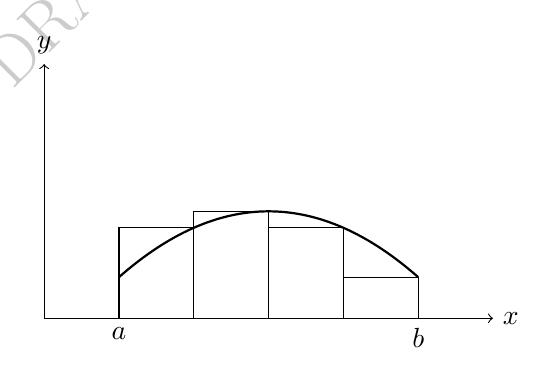
\begin{tikzpicture}[scale=0.95]
\draw[->] (0,0) -- (6,0) node[right] {$x$};
\draw[->] (0,0) -- (0,3.4) node[above] {$y$};
% Interval [a,b] mapped to x in [1,5]
\draw (1,0) node[below] {$a$};
\draw (5,0) node[below] {$b$};
% A smooth schematic curve
\draw[thick,domain=1:5,samples=120,smooth]
plot (\x,{0.22*(\x-1)*(5-\x)+0.55});
% Right-endpoint rectangles for n=4, Delta x = 1 on [1,5]
\foreach \k in {1,2,3,4}{
\pgfmathsetmacro{\xl}{1+(\k-1)}
\pgfmathsetmacro{\xr}{1+\k}
\pgfmathsetmacro{\h}{0.22*(\xr-1)*(5-\xr)+0.55}
\draw[thin] (\xl,0) rectangle (\xr,\h);
}
\end{tikzpicture}
\end{center}

\subsection{Definite Integrals and Basic Properties}

\begin{definition}{Definite integral}{def:definite-integral}
Suppose $f$ is defined on $[a,b]$. Using the equal-width partition with $\Delta x=(b-a)/n$ and sample points $x_i^\ast\in[x_{i-1},x_i]$, the \textbf{definite integral} of $f$ on $[a,b]$ is
\[
\int_a^b f(x)\,dx := \lim_{n\to\infty}\sum_{i=1}^n f(x_i^\ast)\,\Delta x,
\]
provided the limit exists and is independent of the choice of sample points. In that case, $f$ is \textbf{integrable} on $[a,b]$.
\end{definition}

If $f$ changes sign, $\int_a^b f(x)\,dx$ is interpreted as \textbf{net area}: (area above $x$-axis) minus (area below $x$-axis).

\begin{keyformula}[title={Key Formula: Core properties of definite integrals}]
Assume $f,g$ are integrable on $[a,b]$ and $c$ is constant.
\begin{enumerate}[label=(P\arabic*), leftmargin=*]
\item $\displaystyle \int_a^b c\,dx = c(b-a)$.
\item $\displaystyle \int_a^b (f(x)\pm g(x))\,dx = \int_a^b f(x)\,dx \pm \int_a^b g(x)\,dx$.
\item $\displaystyle \int_a^b c f(x)\,dx = c\int_a^b f(x)\,dx$.
\item (Additivity) If $a<c<b$, then $\displaystyle \int_a^b f(x)\,dx = \int_a^c f(x)\,dx + \int_c^b f(x)\,dx$.
\item (Comparison) If $f(x)\ge 0$ on $[a,b]$, then $\displaystyle \int_a^b f(x)\,dx \ge 0$.
\item (Comparison) If $f(x)\ge g(x)$ on $[a,b]$, then $\displaystyle \int_a^b f(x)\,dx \ge \int_a^b g(x)\,dx$.
\item (Bounds) If $m\le f(x)\le M$ on $[a,b]$, then $\displaystyle m(b-a)\le \int_a^b f(x)\,dx \le M(b-a)$.
\end{enumerate}
\end{keyformula}

\begin{examplebox}[title={Worked Example: Average value satisfies its own bounds}]
Show that if $f$ is continuous on $[a,b]$ with $m\le f(x)\le M$, then the average value $\displaystyle f_{\mathrm{ave}}=\frac{1}{b-a}\int_a^b f(x)\,dx$ satisfies $m\le f_{\mathrm{ave}}\le M$.

\textbf{Solution.}
By Property P7,
\[
m(b-a)\le \int_a^b f(x)\,dx \le M(b-a).
\]
Divide by $b-a>0$ to obtain
\[
m \le \frac{1}{b-a}\int_a^b f(x)\,dx \le M,
\]
i.e.\ $m\le f_{\mathrm{ave}}\le M$.
\end{examplebox}

\begin{examtip}[title={Exam Focus: Fast integral comparisons}]
If you can compare integrands pointwise (e.g.\ $f\ge g\ge 0$), then you can compare integrals \emph{without computing antiderivatives}. This is often faster and avoids algebra mistakes.
\end{examtip}

\subsection{The Fundamental Theorem of Calculus}

\textbf{Motivation: Why do we need the FTC?}

At this point in the course, you know two distinct operations:
\begin{itemize}[leftmargin=*]
\item \textbf{Differentiation:} Given a function $f$, compute its instantaneous rate of change $f'(x)$.
\item \textbf{Integration (as area):} Given a function $f$ on $[a,b]$, compute the accumulated area $\int_a^b f(x)\,dx$ by taking the limit of Riemann sums.
\end{itemize}

These look completely unrelated---one is about \emph{rates}, the other is about \emph{totals}. Computing $\int_0^1 x^2\,dx$ from the definition means evaluating $\displaystyle \lim_{n\to\infty}\sum_{i=1}^n \left(\frac{i}{n}\right)^2\cdot\frac{1}{n}$, which requires summation formulas and careful limit-taking.

The Fundamental Theorem of Calculus reveals that differentiation and integration are \textbf{inverse processes}. This has two immediate practical consequences:
\begin{enumerate}[label=(\roman*), leftmargin=*]
\item If you \emph{integrate then differentiate}, you recover the original function (FTC Part~I).
\item If you know an \emph{antiderivative}, you can compute a definite integral instantly without Riemann sums (FTC Part~II).
\end{enumerate}

In effect, the FTC transforms integration from a \emph{limit-of-sums calculation} (slow, algebraically tedious) into an \emph{antiderivative evaluation} (fast, routine). This is why we can evaluate $\int_0^1 x^2\,dx$ by writing $\left[\tfrac{x^3}{3}\right]_0^1 = \tfrac{1}{3}$ instead of summing rectangles.

\vspace{0.5em}

We now state and prove both parts of the theorem carefully, emphasizing \emph{why} each formula takes the form it does.

\begin{theorem}{Fundamental Theorem of Calculus (Part I)}{thm:ftc1}
If $f$ is continuous on $[a,b]$ and
\[
F(x)=\int_a^x f(t)\,dt \qquad (a\le x\le b),
\]
then $F$ is differentiable on $(a,b)$ and
\[
F'(x)=f(x)\qquad (a<x<b).
\]
\end{theorem}

\textbf{Intuition behind Part I: Why does the derivative of an integral give back the original function?}

Think of $F(x)=\int_a^x f(t)\,dt$ as the \textbf{accumulated area} under $y=f(t)$ from $a$ up to $x$. When you increase $x$ by a small amount $h$, the new area is approximately the area of a thin rectangle of width $h$ and height $f(x)$, so
\[
F(x+h)-F(x) \approx f(x)\cdot h.
\]
Dividing by $h$ and taking $h\to 0$ gives $F'(x)=f(x)$. The proof below makes this intuition rigorous using the Mean Value Theorem for Integrals.

\begin{proof}
\textbf{Strategy:} Use the definition of the derivative and then apply the Mean Value Theorem for Integrals to evaluate the resulting integral increment.

\textbf{Step 1: Expand $F'(x)$ using the definition.}

Let $x\in(a,b)$. By definition,
\[
F'(x)=\lim_{h\to 0}\frac{F(x+h)-F(x)}{h}.
\]
Since $F(x)=\int_a^x f(t)\,dt$ and $F(x+h)=\int_a^{x+h} f(t)\,dt$, we have
\[
F(x+h)-F(x) = \int_a^{x+h} f(t)\,dt - \int_a^x f(t)\,dt.
\]
By the additivity property (P4), the interval $[a,x+h]$ splits as $[a,x]\cup[x,x+h]$, giving
\[
F(x+h)-F(x)=\int_x^{x+h} f(t)\,dt.
\]
Therefore
\[
F'(x)=\lim_{h\to 0}\frac{1}{h}\int_x^{x+h} f(t)\,dt.
\]

\textbf{Step 2: Apply the Mean Value Theorem for Integrals.}

Since $f$ is continuous on $[x,x+h]$ (for small $h>0$), the Mean Value Theorem for Integrals guarantees a point $c\in[x,x+h]$ such that
\[
\int_x^{x+h} f(t)\,dt = f(c)\cdot h.
\]
Substituting into our expression for $F'(x)$,
\[
F'(x)=\lim_{h\to 0}\frac{f(c)\cdot h}{h}=\lim_{h\to 0}f(c).
\]

\textbf{Step 3: Take the limit as $h\to 0$.}

Because $c\in[x,x+h]$, as $h\to 0$ we have $c\to x$ (the point $c$ is squeezed between $x$ and $x+h$). Since $f$ is continuous at $x$,
\[
\lim_{h\to 0}f(c)=f(x).
\]
Hence $F'(x)=f(x)$, as desired.
\end{proof}

\textbf{Why is continuity of $f$ required?}

The proof relies on two facts:
\begin{itemize}[leftmargin=*]
\item The Mean Value Theorem for Integrals, which requires $f$ to be continuous.
\item The limit $\lim_{c\to x}f(c)=f(x)$, which is the definition of continuity at $x$.
\end{itemize}
If $f$ has a jump discontinuity, the accumulated area function $F(x)$ may still be continuous, but it will fail to be differentiable at the jump.

\vspace{0.5em}

\textbf{Summary of Part I in words:} If $F(x)$ accumulates the values of $f$ from $a$ to $x$, then the \emph{rate of change} of this accumulation at $x$ is precisely $f(x)$ itself.

\begin{examplebox}[title={Worked Example: FTC Part I (direct application)}]
Find $\displaystyle \frac{d}{dx}\int_1^x \frac{1}{1+t^2}\,dt$.

\textbf{Solution.}
The integrand $f(t)=\frac{1}{1+t^2}$ is continuous on $\mathbb{R}$. By FTC Part I, with $a=1$,
\[
\frac{d}{dx}\int_1^x \frac{1}{1+t^2}\,dt = f(x)=\frac{1}{1+x^2}.
\]
\end{examplebox}

\begin{examplebox}[title={Worked Example: FTC Part I with Chain Rule}]
Find $\displaystyle \frac{d}{dx}\int_1^{x^4} \sec t\,dt$.

\textbf{Solution.}
Let $u=x^4$. Then
\[
\frac{d}{dx}\int_1^{x^4} \sec t\,dt = \frac{d}{dx}\int_1^u \sec t\,dt = \frac{d}{du}\left(\int_1^u \sec t\,dt\right)\cdot \frac{du}{dx}.
\]
By FTC Part I, $\displaystyle \frac{d}{du}\int_1^u \sec t\,dt = \sec u$. Since $\frac{du}{dx}=4x^3$, we obtain
\[
\frac{d}{dx}\int_1^{x^4} \sec t\,dt = \sec(x^4)\cdot 4x^3 = 4x^3\sec(x^4).
\]
\end{examplebox}

\begin{examplebox}[title={Worked Example: FTC Part I with two variable limits (Leibniz rule)}]
Find $\displaystyle \frac{d}{dx}\int_{x}^{x^2} \sin t\,dt$.

\textbf{Solution.}
\textbf{Method:} Split the integral at a fixed point (say, $0$) and apply FTC Part I to each piece.

Write
\[
\int_x^{x^2} \sin t\,dt = \int_x^0 \sin t\,dt + \int_0^{x^2} \sin t\,dt = -\int_0^x \sin t\,dt + \int_0^{x^2} \sin t\,dt.
\]
Differentiate term-by-term using FTC Part I and the Chain Rule:
\[
\frac{d}{dx}\left(-\int_0^x \sin t\,dt\right)=-\sin x,
\]
\[
\frac{d}{dx}\int_0^{x^2} \sin t\,dt = \sin(x^2)\cdot 2x.
\]
Hence
\[
\frac{d}{dx}\int_x^{x^2} \sin t\,dt = -\sin x + 2x\sin(x^2).
\]

\textbf{General form (Leibniz rule):}
\[
\frac{d}{dx}\int_{a(x)}^{b(x)} f(t)\,dt = f(b(x))\cdot b'(x) - f(a(x))\cdot a'(x).
\]
\end{examplebox}

\begin{examtip}[title={Exam Focus: Variable limits and Chain Rule}]
When the upper limit is not just $x$ but a composite function $g(x)$, you \emph{must} apply the Chain Rule:
\[
\frac{d}{dx}\int_a^{g(x)} f(t)\,dt = f(g(x))\cdot g'(x).
\]
When both limits are variable, split at a convenient constant and differentiate each piece separately.
\end{examtip}

\vspace{1em}

\begin{theorem}{Fundamental Theorem of Calculus (Part II)}{thm:ftc2}
If $f$ is continuous on $[a,b]$ and $F$ is \emph{any} antiderivative of $f$ (i.e., $F'(x)=f(x)$ on $[a,b]$), then
\[
\int_a^b f(x)\,dx = F(b)-F(a).
\]
\end{theorem}

\textbf{Intuition behind Part II: Why does an antiderivative let us evaluate definite integrals?}

Part I showed that the accumulation function $G(x)=\int_a^x f(t)\,dt$ is an antiderivative of $f$. If $F$ is \emph{any other} antiderivative of $f$, then $F$ and $G$ differ by a constant (Theorem~\ref{thm:antiderivatives-constant}):
\[
F(x)=G(x)+C.
\]
Evaluating at $x=b$,
\[
F(b)=G(b)+C=\int_a^b f(t)\,dt + C.
\]
Evaluating at $x=a$,
\[
F(a)=G(a)+C=\int_a^a f(t)\,dt + C = 0+C=C.
\]
Subtracting,
\[
F(b)-F(a)=\int_a^b f(t)\,dt.
\]
The constant $C$ cancels in the subtraction, which is why you can use \emph{any} antiderivative $F$ (with or without $+C$) to compute the definite integral.

\begin{proof}
\textbf{Strategy:} Define $G(x)=\int_a^x f(t)\,dt$. Both $G$ and $F$ are antiderivatives of $f$, so they differ by a constant. Exploit this to relate $\int_a^b f$ to $F(b)-F(a)$.

By FTC Part I, $G'(x)=f(x)$ on $(a,b)$. Since $F$ is also an antiderivative of $f$, we have $F'(x)=f(x)=G'(x)$ on $(a,b)$. By Theorem~\ref{thm:antiderivatives-constant}, there exists a constant $C$ such that
\[
F(x)=G(x)+C \qquad \text{for all }x\in[a,b].
\]

Evaluate at $x=b$:
\[
F(b)=G(b)+C=\int_a^b f(t)\,dt + C.
\]
Evaluate at $x=a$:
\[
F(a)=G(a)+C=\int_a^a f(t)\,dt + C = 0+C=C.
\]
Subtract the second equation from the first:
\[
F(b)-F(a)=\int_a^b f(t)\,dt.
\]
\end{proof}

\textbf{Why is the dummy variable irrelevant?}

In the statement of the theorem, we wrote $\int_a^b f(x)\,dx$ instead of $\int_a^b f(t)\,dt$. The choice of variable inside the integral doesn't matter:
\[
\int_a^b f(x)\,dx = \int_a^b f(t)\,dt = \int_a^b f(u)\,du.
\]
All represent the same number (the accumulated area from $a$ to $b$). The variable is a \textbf{dummy variable}---it is local to the integral and does not appear in the final answer $F(b)-F(a)$.

\vspace{0.5em}

\textbf{Notation:} We often write $F(b)-F(a)$ as $\left[F(x)\right]_a^b$ or $F(x)\Big|_a^b$.

\begin{examplebox}[title={Worked Example: FTC Part II (direct evaluation)}]
Evaluate $\displaystyle \int_{-1}^{2} x^3\,dx$.

\textbf{Solution.}
An antiderivative of $f(x)=x^3$ is $F(x)=\frac{x^4}{4}$ (we omit $+C$ because it will cancel). By FTC Part II,
\[
\int_{-1}^{2} x^3\,dx = \left[\frac{x^4}{4}\right]_{-1}^{2} = \frac{2^4}{4}-\frac{(-1)^4}{4}=\frac{16}{4}-\frac{1}{4}=\frac{15}{4}.
\]
\end{examplebox}

\begin{examplebox}[title={Worked Example: FTC Part II with endpoint checks}]
Evaluate $\displaystyle \int_0^\pi \cos x\,dx$.

\textbf{Solution.}
An antiderivative of $\cos x$ is $\sin x$. Hence
\[
\int_0^\pi \cos x\,dx = \left[\sin x\right]_0^\pi = \sin\pi - \sin 0 = 0-0=0.
\]

\textbf{Interpretation:} The area above the $x$-axis on $[0,\tfrac{\pi}{2}]$ exactly cancels the area below the $x$-axis on $[\tfrac{\pi}{2},\pi]$, giving net area zero.
\end{examplebox}

\begin{examplebox}[title={Worked Example: FTC Part II with absolute value (sign change)}]
Evaluate $\displaystyle \int_{-2}^2 |x|\,dx$.

\textbf{Solution.}
The function $|x|$ is not differentiable at $x=0$, so we must split the integral at the point where the formula changes:
\[
\int_{-2}^2 |x|\,dx = \int_{-2}^0 (-x)\,dx + \int_0^2 x\,dx.
\]
Compute each piece:
\[
\int_{-2}^0 (-x)\,dx = \left[-\frac{x^2}{2}\right]_{-2}^0 = 0-\left(-\frac{4}{2}\right)=2,
\]
\[
\int_0^2 x\,dx = \left[\frac{x^2}{2}\right]_0^2 = 2-0=2.
\]
Hence $\displaystyle \int_{-2}^2 |x|\,dx = 2+2=4$.

\textbf{Sanity check:} By symmetry, the two halves contribute equally; each is a triangle of base~2 and height~2, so area $\tfrac{1}{2}(2)(2)=2$.
\end{examplebox}

\begin{commonmistake}[title={Common Mistake: Ignoring sign changes in the integrand}]
If $f$ changes sign or formula on $[a,b]$, you \emph{cannot} apply FTC Part II blindly to $\int_a^b f(x)\,dx$. You must:
\begin{enumerate}[label=(\arabic*)]
\item Identify points $c$ where $f$ changes sign or formula.
\item Split the integral: $\int_a^b f = \int_a^c f + \int_c^b f$.
\item Evaluate each piece separately using the correct formula for $f$ on each subinterval.
\end{enumerate}
Example: $\int_{-1}^1 \frac{1}{x}\,dx$ is \textbf{not} $\ln|x|\big|_{-1}^1 = 0$. The integrand has a singularity at $x=0$; the integral is improper and divergent.
\end{commonmistake}

\begin{examtip}[title={Exam Focus: FTC Part II workflow}]
When evaluating $\int_a^b f(x)\,dx$:
\begin{enumerate}[label=(\arabic*), leftmargin=*]
\item Find \emph{any} antiderivative $F(x)$ of $f(x)$ (omit $+C$).
\item Compute $F(b)-F(a)$.
\item Sanity check:
\begin{itemize}[leftmargin=2em]
\item If $f\ge 0$ on $[a,b]$, the answer should be $\ge 0$.
\item If $f$ is odd and the interval is symmetric, the answer may be zero.
\item If $f$ changes sign, check that you've split correctly.
\end{itemize}
\end{enumerate}
\end{examtip}

\begin{examtip}[title={Exam Focus: When to use Part I vs.\ Part II}]
\textbf{Use FTC Part I when:}
\begin{itemize}[leftmargin=*]
\item You see $\displaystyle \frac{d}{dx}\int_a^{g(x)} f(t)\,dt$ (differentiate an integral).
\item The question asks for the derivative of an accumulation function.
\end{itemize}
\textbf{Use FTC Part II when:}
\begin{itemize}[leftmargin=*]
\item You need to evaluate $\int_a^b f(x)\,dx$ numerically.
\item You are asked to compute a definite integral using an antiderivative.
\end{itemize}
\end{examtip}

\subsection{The Substitution Rule}

Integration by substitution (also called $u$-substitution) is the reverse of the Chain Rule for differentiation. It allows us to evaluate integrals by transforming them into simpler integrals in a new variable.

\begin{theorem}{Substitution Rule (Indefinite Integrals)}{thm:substitution-indefinite}
If $u=g(x)$ is differentiable and $F$ is an antiderivative of $f$, then
\[
\int f(g(x))\,g'(x)\,dx = F(g(x))+C.
\]
Equivalently, writing $du=g'(x)\,dx$,
\[
\int f(u)\,du = F(u)+C.
\]
\end{theorem}

\textbf{Practical recipe:}
\begin{enumerate}[label=(\arabic*)]
\item Choose a substitution $u=g(x)$.
\item Compute $du=g'(x)\,dx$.
\item Rewrite the integrand and differential in terms of $u$ and $du$.
\item Integrate with respect to $u$.
\item Substitute back $u=g(x)$ to express the answer in terms of $x$.
\end{enumerate}

\begin{examplebox}[title={Worked Example: $u$-substitution for indefinite integrals}]
Evaluate $\displaystyle \int x\cos(x^2)\,dx$.

\textbf{Solution.}
Let $u=x^2$. Then $du=2x\,dx$, so $x\,dx=\frac{1}{2}du$. Substitute:
\[
\int x\cos(x^2)\,dx = \int \cos u\cdot \frac{1}{2}\,du = \frac{1}{2}\sin u + C = \frac{1}{2}\sin(x^2)+C.
\]
\end{examplebox}

\begin{theorem}{Substitution Rule (Definite Integrals)}{thm:substitution-definite}
If $g$ is continuously differentiable on $[a,b]$ and $f$ is continuous on the range of $g$, then
\[
\int_a^b f(g(x))\,g'(x)\,dx = \int_{g(a)}^{g(b)} f(u)\,du.
\]
\end{theorem}

\textbf{Key observation:} When you substitute $u=g(x)$ in a definite integral, you must also transform the limits of integration: $x=a$ becomes $u=g(a)$, and $x=b$ becomes $u=g(b)$.

\begin{examplebox}[title={Worked Example: $u$-substitution for definite integrals}]
Evaluate $\displaystyle \int_2^5 \frac{1}{3-5x}\,dx$.

\textbf{Solution.}
Let $u=3-5x$. Then $du=-5\,dx$, so $dx=-\frac{1}{5}du$.

Transform the limits:
\[
x=2 \Rightarrow u=3-5(2)=-7,\qquad x=5 \Rightarrow u=3-5(5)=-22.
\]
Substitute:
\[
\int_2^5 \frac{1}{3-5x}\,dx = \int_{-7}^{-22} \frac{1}{u}\cdot \left(-\frac{1}{5}\right)\,du = -\frac{1}{5}\int_{-7}^{-22} \frac{1}{u}\,du.
\]
Reverse the limits (introduces a minus sign):
\[
= \frac{1}{5}\int_{-22}^{-7} \frac{1}{u}\,du = \frac{1}{5}\left[\ln|u|\right]_{-22}^{-7} = \frac{1}{5}\bigl(\ln 7 - \ln 22\bigr)=\frac{1}{5}\ln\left(\frac{7}{22}\right).
\]
\end{examplebox}

\begin{examtip}[title={Exam Focus: Substitution workflow for definite integrals}]
When using substitution on $\int_a^b f(x)\,dx$:
\begin{enumerate}[label=(\arabic*), leftmargin=*]
\item Choose $u=g(x)$ and compute $du=g'(x)\,dx$.
\item Transform limits: $u_1=g(a)$, $u_2=g(b)$.
\item Rewrite the integral entirely in terms of $u$ (no $x$ should remain).
\item Integrate with respect to $u$ from $u_1$ to $u_2$.
\item \textbf{Do not} substitute back to $x$---evaluate directly in $u$.
\end{enumerate}
\end{examtip}

\newpage
\subsection{Improper Integrals}

So far, we have defined $\int_a^b f(x)\,dx$ only when $[a,b]$ is a finite interval and $f$ is continuous (or at least bounded and integrable) on $[a,b]$. An \textbf{improper integral} extends the concept of integration to:
\begin{itemize}
\item \textbf{Type 1:} Infinite intervals (e.g., $\int_1^\infty \frac{1}{x^2}\,dx$).
\item \textbf{Type 2:} Unbounded integrands (e.g., $\int_0^1 \frac{1}{\sqrt{x}}\,dx$, where $f(x)\to\infty$ as $x\to 0^+$).
\end{itemize}

\begin{definition}{Improper Integral of Type 1 (Infinite Interval)}{def:improper-type1}
\begin{enumerate}[label=(\alph*), leftmargin=*]
\item If $\int_a^t f(x)\,dx$ exists for all $t\ge a$, then
\[
\int_a^\infty f(x)\,dx := \lim_{t\to\infty}\int_a^t f(x)\,dx.
\]
\item If $\int_t^b f(x)\,dx$ exists for all $t\le b$, then
\[
\int_{-\infty}^b f(x)\,dx := \lim_{t\to-\infty}\int_t^b f(x)\,dx.
\]
\item If both $\int_{-\infty}^a f$ and $\int_a^\infty f$ converge, then
\[
\int_{-\infty}^\infty f(x)\,dx := \int_{-\infty}^a f(x)\,dx + \int_a^\infty f(x)\,dx.
\]
\end{enumerate}
In each case, the integral \textbf{converges} if the limit exists (and is finite); otherwise it \textbf{diverges}.
\end{definition}

\begin{keyformula}[title={Key Formula: $p$-integrals (Type 1 and Type 2)}]
\[
\int_1^\infty \frac{1}{x^p}\,dx \text{ converges } \iff p>1,
\qquad
\int_0^1 \frac{1}{x^p}\,dx \text{ converges } \iff p<1.
\]
\end{keyformula}

% Figure description (fallback): Plot of y=1/x^2 for x>=1, decreasing to 0; the "tail area" from 1 to infinity is finite, illustrating a convergent improper integral.

\begin{center}
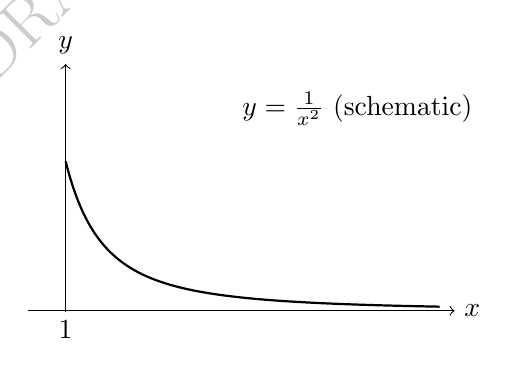
\begin{tikzpicture}[scale=0.95]
\draw[->] (0.5,0) -- (6.2,0) node[right] {$x$};
\draw[->] (1,0) -- (1,3.3) node[above] {$y$};
\draw (1,0) node[below] {$1$};
\draw[thick,domain=1:6,samples=120,smooth]
plot (\x,{2/(\x*\x)});
\draw[dashed] (1,2) -- (1,0);
\node at (4.9,2.7) {$y=\frac{1}{x^2}$ (schematic)};
\end{tikzpicture}
\end{center}

\begin{examplebox}[title={Worked Example: Type 1 divergence}]
Determine whether $\displaystyle \int_1^\infty \frac{1}{x}\,dx$ converges.

\textbf{Solution.}
Write the definition:
\[
\int_1^\infty \frac{1}{x}\,dx=\lim_{t\to\infty}\int_1^t \frac{1}{x}\,dx
=\lim_{t\to\infty}\bigl[\ln|x|\bigr]_{1}^{t}
=\lim_{t\to\infty}\ln t=\infty.
\]
Hence the improper integral \textbf{diverges}.
\end{examplebox}

\begin{examplebox}[title={Worked Example: Type 1 evaluation (split correctly)}]
Evaluate $\displaystyle \int_{-\infty}^{\infty}\frac{1}{1+x^2}\,dx$.

\textbf{Solution.}
Split at $0$ and take one-sided limits:
\[
\int_{-\infty}^{\infty}\frac{1}{1+x^2}\,dx
=\int_{-\infty}^{0}\frac{1}{1+x^2}\,dx+\int_{0}^{\infty}\frac{1}{1+x^2}\,dx,
\]
provided both sides converge.

Since $\int \frac{1}{1+x^2}\,dx=\tan^{-1}x+C$,
\[
\int_{0}^{\infty}\frac{1}{1+x^2}\,dx=\lim_{t\to\infty}\bigl[\tan^{-1}x\bigr]_0^t
=\frac{\pi}{2},
\qquad
\int_{-\infty}^{0}\frac{1}{1+x^2}\,dx=\lim_{t\to-\infty}\bigl[\tan^{-1}x\bigr]_t^0
=\frac{\pi}{2}.
\]
Therefore $\displaystyle \int_{-\infty}^{\infty}\frac{1}{1+x^2}\,dx=\pi$.
\end{examplebox}

\begin{definition}{Improper Integral of Type 2 (Unbounded Integrand)}{def:improper-type2}
\begin{enumerate}[label=(\alph*), leftmargin=*]
\item If $f$ is continuous on $[a,b)$ and $\lim_{x\to b^-}f(x)=\pm\infty$, then
\[
\int_a^b f(x)\,dx := \lim_{t\uparrow b}\int_a^t f(x)\,dx.
\]
\item If $f$ is continuous on $(a,b]$ and $\lim_{x\to a^+}f(x)=\pm\infty$, then
\[
\int_a^b f(x)\,dx := \lim_{t\downarrow a}\int_t^b f(x)\,dx.
\]
\item If $f$ has a discontinuity at $c\in(a,b)$ and both $\int_a^c f$ and $\int_c^b f$ (as improper integrals) converge, then
\[
\int_a^b f(x)\,dx := \int_a^c f(x)\,dx + \int_c^b f(x)\,dx.
\]
\end{enumerate}
The integral converges if the limit(s) exist and are finite; otherwise it diverges.
\end{definition}

\begin{examplebox}[title={Worked Example: Type 2 at an endpoint}]
Evaluate $\displaystyle \int_{2}^{5}\frac{1}{\sqrt{x-2}}\,dx$.

\textbf{Solution.}
This is improper at $x=2$. By definition,
\[
\int_{2}^{5}\frac{1}{\sqrt{x-2}}\,dx=\lim_{t\downarrow 2}\int_{t}^{5}\frac{1}{\sqrt{x-2}}\,dx.
\]
Let $u=x-2$ so $du=dx$. Then $\int u^{-1/2}\,du = 2u^{1/2}$, hence
\[
\int_{t}^{5}\frac{1}{\sqrt{x-2}}\,dx
= \left[2\sqrt{x-2}\right]_{t}^{5}
=2\sqrt{3}-2\sqrt{t-2}.
\]
Taking $t\downarrow 2$ gives $2\sqrt{t-2}\to 0$, so the integral converges and equals $2\sqrt{3}$.
\end{examplebox}

\begin{commonmistake}[title={Common Mistake: Treating $\int_{-\infty}^{\infty}$ as a symmetric single limit}]
The definition is \emph{not} $\lim_{A\to\infty}\int_{-A}^{A} f(x)\,dx$.

A two-sided improper integral converges only if \textbf{both} one-sided integrals converge:
\[
\int_{-\infty}^{\infty} f := \int_{-\infty}^{a} f + \int_a^{\infty} f,
\quad \text{with both terms finite.}
\]
Symmetric cancellation can produce a finite number even when the improper integral diverges (see extension below).
\end{commonmistake}

\begin{examtip}[title={Exam Focus: Improper integrals (non-negotiable workflow)}]
\begin{enumerate}[label=(\arabic*), leftmargin=*]
\item Identify why it is improper (infinite interval / unbounded integrand / interior singularity).
\item Rewrite using the correct one-sided limit(s) \emph{before} manipulating.
\item Decide convergence; only then compute the finite value (if it converges).
\end{enumerate}
\end{examtip}

\begin{extension}[title={Extension (Tutorial 3, Question 2, Method 1)}]
\textbf{Syllabus link:} Chapter 1 — \emph{§1.6 Improper Integrals}.\\
\textbf{Proposition (independence of split point).}

Assume that for every real $c$, both $\int_{-\infty}^{c} f(x)\,dx$ and $\int_{c}^{\infty} f(x)\,dx$ converge.
Then for any real $a,b$,
\[
\int_{-\infty}^{a} f(x)\,dx+\int_{a}^{\infty} f(x)\,dx
=
\int_{-\infty}^{b} f(x)\,dx+\int_{b}^{\infty} f(x)\,dx.
\]

\textbf{Proof.} WLOG let $a<b$. For $M>0$, finite additivity gives
\[
\int_{-M}^{b} f=\int_{-M}^{a} f+\int_{a}^{b} f.
\]
Take $M\to\infty$ (the limits exist by hypothesis) to obtain
\[
\int_{-\infty}^{b} f=\int_{-\infty}^{a} f+\int_{a}^{b} f. \tag{1}
\]
Similarly, for $N>0$, finite additivity gives $\int_{a}^{N} f=\int_{a}^{b} f+\int_{b}^{N} f$; letting $N\to\infty$ yields
\[
\int_{a}^{\infty} f=\int_{a}^{b} f+\int_{b}^{\infty} f. \tag{2}
\]
Rearrange (2) as $\int_{b}^{\infty} f=\int_{a}^{\infty} f-\int_{a}^{b} f$ and add to (1):
\[
\int_{-\infty}^{b} f+\int_{b}^{\infty} f
=\left(\int_{-\infty}^{a} f+\int_{a}^{b} f\right)+\left(\int_{a}^{\infty} f-\int_{a}^{b} f\right)
=\int_{-\infty}^{a} f+\int_{a}^{\infty} f.
\]
\end{extension}

\begin{extension}[title={Extension (Beyond Syllabus: Cauchy principal value vs.\ improper integral)}]
\textbf{Syllabus link:} Chapter 1 — \emph{§1.6 Improper Integrals}.\\
\textbf{Definition.} For integrable $f$ on every finite interval, the \emph{Cauchy principal value} is
\[
\operatorname{PV}\!\int_{-\infty}^{\infty} f(x)\,dx := \lim_{A\to\infty}\int_{-A}^{A} f(x)\,dx
\quad\text{(if the limit exists).}
\]
This is \emph{not} the same as the improper integral, which requires both $\int_{-\infty}^{0} f$ and $\int_{0}^{\infty} f$ to converge (finite).\\
\textbf{Example (odd integrand with finite PV but divergent improper integral).}

Let $f(x)=\frac{x}{1+x^2}$ (odd, continuous on $\mathbb{R}$).
Compute one-sided integrals:
\[
\int_{0}^{A}\frac{x}{1+x^2}\,dx=\left[\frac12\ln(1+x^2)\right]_{0}^{A}=\frac12\ln(1+A^2)\xrightarrow[A\to\infty]{}\infty,
\]
\[
\int_{-A}^{0}\frac{x}{1+x^2}\,dx=\left[\frac12\ln(1+x^2)\right]_{-A}^{0}= -\frac12\ln(1+A^2)\xrightarrow[A\to\infty]{}-\infty.
\]
Hence the improper integral $\int_{-\infty}^{\infty} f$ \emph{does not converge} (one-sided integrals are not both finite).

But for every $A>0$, oddness gives $\int_{-A}^{A} f(x)\,dx=0$, so
\[
\operatorname{PV}\!\int_{-\infty}^{\infty}\frac{x}{1+x^2}\,dx=\lim_{A\to\infty}0=0.
\]
\end{extension}

%==================================================
% USER COMMENTS (EDITABLE)
%==================================================
% The FTC section has been enhanced with:
% - A motivational paragraph explaining *why* the FTC is needed (bridging rates and totals).
% - Intuition paragraphs *before* each part, explaining the geometric/physical reasoning.
% - Detailed proof annotations with step-by-step strategy and "why this works" commentary.
% - Explicit discussion of continuity hypothesis and dummy-variable conventions.
% - Additional worked examples with FTC Part I (Chain Rule, Leibniz rule) and Part II (absolute value, sign-change splitting).
% - Common mistakes and exam tips focusing on when to use Part I vs Part II, and how to handle variable limits.
% - All existing content preserved; only explanatory material and examples added.
%
% User request: "add explanation to the FTC part especially, avoid giving the definitions directly without any explanation on why are they like that"
% This has been addressed by:
%   1. Adding a "Motivation" subsection before the FTC theorems.
%   2. Including "Intuition behind Part I" and "Intuition behind Part II" paragraphs that explain the geometric/physical meaning *before* the formal statements.
%   3. Annotating the proofs with strategy comments and step-by-step reasoning.
%   4. Adding "Why is X required?" discussions after each theorem.
%   5. Including multiple worked examples demonstrating Chain Rule, Leibniz rule, absolute values, and sanity checks.
%==================================================

%==================================================
% MH1101 Calculus II — Chapter 2 Notes
% File: chapters/ch02_applications_of_integrals.tex
%==================================================

\newpage
\section{Applications of Integrals}

\subsection{Area Between Curves}

Many geometry questions reduce to (i) identifying the correct bounding curves/lines, (ii) locating intersection points, and (iii) setting up a \emph{nonnegative} integrand (area is never negative).

\textbf{Motivation: From ``area under a curve'' to ``area between curves.''}

In Chapter~1 we saw that $\int_a^b f(x)\,dx$ gives the \emph{signed} area between $y=f(x)$ and the $x$-axis. What if we want the area of a region enclosed between \emph{two} curves $y=f(x)$ and $y=g(x)$? The idea is simple: at each $x$, the vertical ``height'' of the region is $(f(x)-g(x))$ (assuming $f$ is on top). Summing these infinitesimal vertical strips gives the total area. This is exactly how the Riemann-sum derivation works:
\begin{itemize}[leftmargin=*]
\item Divide $[a,b]$ into $n$ strips of width $\Delta x$.
\item Each strip is approximately a rectangle of width $\Delta x$ and height $f(x_i)-g(x_i)$.
\item Summing and taking $n\to\infty$ gives $A=\int_a^b(f(x)-g(x))\,dx$.
\end{itemize}
The requirement $f(x)\ge g(x)$ ensures every strip has nonneg\-ative height, so we get geometric (unsigned) area.

\begin{theorem}{Area between two curves (w.r.t.\ $x$)}{thm:area-between-curves-x}
Let $f,g$ be continuous on $[a,b]$ and suppose $f(x)\ge g(x)$ for all $x\in[a,b]$.
The area of the region bounded by $y=f(x)$, $y=g(x)$, $x=a$, $x=b$ is
\[
A=\int_a^b \bigl(f(x)-g(x)\bigr)\,dx.
\]
\end{theorem}

\textbf{Why ``top minus bottom''?}
The integrand $(f-g)$ measures the \emph{vertical distance} between the two curves at position $x$. If $f(x)\ge g(x)$ on the whole interval, this distance is nonneg\-ative and we get a single integral. If the ordering swaps (i.e., $g$ is on top for part of the interval), the integrand $(f-g)$ becomes negative there, yielding signed area rather than geometric area. To get geometric area, you must \textbf{split} at intersection points and always write $(\text{top}-\text{bottom})\ge 0$.

\begin{keyformula}[title={Key Formula: Area Between Curves (Choose $dx$ or $dy$)}]
\begin{itemize}[leftmargin=*]
\item \textbf{Vertical slices ($dx$):}\quad $A=\displaystyle\int_{x=a}^{x=b}(\text{top}-\text{bottom})\,dx$.
\item \textbf{Horizontal slices ($dy$):}\quad $A=\displaystyle\int_{y=c}^{y=d}(\text{right}-\text{left})\,dy$.
\item \textbf{Workflow:}\quad find intersection points $\Rightarrow$ split the interval whenever the ordering (top/bottom or right/left) changes.
\end{itemize}
\end{keyformula}

\textbf{When to use $dx$ vs.\ $dy$:}

The choice is a matter of convenience, not correctness. Ask yourself:
\begin{itemize}[leftmargin=*]
\item Can I express both boundaries as functions of a \emph{single} variable with \emph{one} formula each? If yes, integrate with respect to that variable.
\item Does one choice avoid splitting the integral? For example, a parabola $x=y^2$ and a line $x=y+2$ are simpler to integrate with $dy$ (one integral from $y=-1$ to $y=2$), whereas using $dx$ would require two separate integrals.
\end{itemize}

% Figure description (fallback): Plot y=sin x and y=cos x on [0,pi/2]; they intersect at x=pi/4; split the area into two parts since top/bottom swaps at pi/4.

\begin{center}
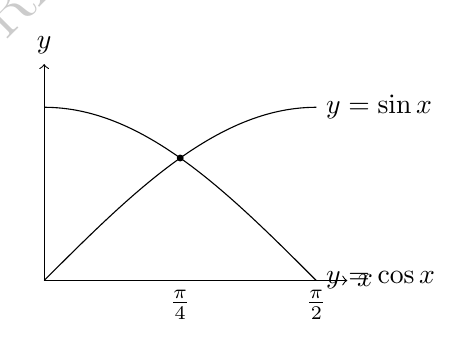
\begin{tikzpicture}[scale=2.2]
\draw[->] (0,0) -- (1.75,0) node[right] {$x$};
\draw[->] (0,0) -- (0,1.25) node[above] {$y$};
\draw (1.5708,0) node[below] {$\frac{\pi}{2}$};
\draw (0.7854,0) node[below] {$\frac{\pi}{4}$};
\draw[domain=0:1.5708, samples=80] plot (\x,{sin(deg(\x))}) node[right] {$y=\sin x$};
\draw[domain=0:1.5708, samples=80] plot (\x,{cos(deg(\x))}) node[right] {$y=\cos x$};
\fill (0.7854,0.7071) circle (0.02);
\end{tikzpicture}
\end{center}

\begin{examplebox}[title={Worked Example (Lecture Example 2.2): $y=\sin x$ vs.\ $y=\cos x$ on $[0,\tfrac{\pi}{2}]$}]
Find the area bounded by $y=\sin x$, $y=\cos x$, $x=0$, $x=\frac{\pi}{2}$.

\textbf{Solution.}
Solve $\sin x=\cos x\Rightarrow x=\frac{\pi}{4}$ on $[0,\frac{\pi}{2}]$.
On $[0,\frac{\pi}{4}]$, $\cos x\ge \sin x$; on $[\frac{\pi}{4},\frac{\pi}{2}]$, $\sin x\ge \cos x$. Hence
\begin{align*}
A
&=\int_{0}^{\pi/4}(\cos x-\sin x)\,dx+\int_{\pi/4}^{\pi/2}(\sin x-\cos x)\,dx\\
&=\bigl[\sin x+\cos x\bigr]_{0}^{\pi/4}+\bigl[-\cos x-\sin x\bigr]_{\pi/4}^{\pi/2}
= \bigl(\sqrt2-1\bigr)+\bigl(\sqrt2-1\bigr)\\
&=2\sqrt2-2.
\end{align*}
\end{examplebox}

\begin{examplebox}[title={Worked Example (Lecture Example 2.1): $y=x^2+1$ vs.\ $y=x$ on $[0,1]$}]
Find the area bounded above by $y=x^2+1$, below by $y=x$, and on the sides by $x=0$ and $x=1$.

\textbf{Solution.}
First check ordering: for $x\in[0,1]$, $x^2+1\ge 1> x$ (since $x\le 1$), so $f(x)=x^2+1$ is on top throughout. No splitting needed.
\[
A=\int_0^1 \bigl((x^2+1)-x\bigr)\,dx
=\int_0^1 (x^2-x+1)\,dx
=\left[\frac{x^3}{3}-\frac{x^2}{2}+x\right]_0^1
=\frac{1}{3}-\frac{1}{2}+1=\frac{5}{6}.
\]

\textbf{Sanity check:} The region lies inside the unit square $[0,1]\times[0,2]$, so $A<2$. Also $A>0$ since the integrand is positive.\ $\checkmark$
\end{examplebox}

\begin{examplebox}[title={Worked Example: Horizontal slices ($dy$) are simpler (Tutorial 3, Q3(b) style)}]
Find the area enclosed by the parabola $4x+y^2=12$ and the line $x=y$.

\textbf{Solution.}
Rewrite the parabola as $x=3-\tfrac{y^2}{4}$, and the line as $x=y$.

\textbf{Intersections:} Set $y=3-\tfrac{y^2}{4}$, i.e.\ $y^2+4y-12=0$, so $(y+6)(y-2)=0$, giving $y=-6$ and $y=2$.

For $y\in[-6,2]$, the parabola lies to the \emph{right} of the line (check: at $y=0$, parabola gives $x=3$, line gives $x=0$). Hence

\[
A=\int_{-6}^{2}\left[\left(3-\frac{y^2}{4}\right)-y\right]\,dy
=\int_{-6}^{2}\left(3-y-\frac{y^2}{4}\right)\,dy.
\]

Evaluate:
\[
=\left[3y-\frac{y^2}{2}-\frac{y^3}{12}\right]_{-6}^{2}
=\left(6-2-\frac{8}{12}\right)-\left(-18-18+18\right)
=\frac{10}{3}-(-18)=\frac{64}{3}.
\]

Using $dx$ would require solving for $y$ (two branches $y=\pm\sqrt{12-4x}$) and splitting the integral at $x=-6$ and $x=2$---much messier. This illustrates why choosing the right variable matters.
\end{examplebox}

\begin{commonmistake}[title={Common Mistake: Not Splitting Where the Curves Cross}]
If the ``top'' and ``bottom'' curves swap order inside $[a,b]$, then $\int_a^b(f-g)\,dx$ gives \emph{signed area}, not geometric area.
Always find intersection points first and split accordingly.
\end{commonmistake}

\begin{commonmistake}[title={Common Mistake: Forgetting to check the ordering}]
Even if you correctly find intersection points, you still need to determine \emph{which curve is on top} in each sub-interval. A quick way: plug in a test value of $x$ (or $y$) from each sub-interval and compare.

For instance, between $y=x^3$ and $y=x$ on $[-1,1]$: the intersections are $x=-1,0,1$. On $(-1,0)$, test $x=-0.5$: $(-0.5)^3=-0.125$ vs.\ $-0.5$, so $x^3>x$ there. On $(0,1)$, test $x=0.5$: $0.125<0.5$, so $x>x^3$. The ordering reverses.
\end{commonmistake}

\begin{examtip}[title={Exam Focus: Fast Setup Checklist for Area Problems}]
\begin{itemize}[leftmargin=*]
\item Sketch \emph{roughly} and label intersections (solve algebraically).
\item Decide $dx$ vs.\ $dy$ by whichever gives \textbf{simpler bounds and simpler integrand}.
\item Write the integrand explicitly as \textbf{(top$-$bottom)} or \textbf{(right$-$left)} and ensure it is $\ge 0$ on each sub-interval.
\end{itemize}
\end{examtip}

\begin{extension}[title={Extension (Beyond Syllabus: absolute-value area formula)}]
\textbf{Syllabus link:} Chapter 2 — 2.1 Area Between Curves.

\textbf{Proposition.} Let $f,g$ be continuous on $[a,b]$. Assume there exists a partition
$a=x_0<x_1<\cdots<x_n=b$ such that $f-g$ does not change sign on each $(x_{k-1},x_k)$. Then the area between the two curves is
\[
A = \int_a^b |f(x)-g(x)|\,dx = \sum_{k=1}^n \left|\int_{x_{k-1}}^{x_k}(f(x)-g(x))\,dx\right|.
\]
This is just the rigorous statement of ``split and take absolute values.'' It can simplify setup when $f-g$ factors nicely.
\end{extension}

\newpage
\subsection{Volumes by Disk/Washer Method}

\textbf{Motivation: From area to volume via slicing.}

We already know how to compute areas of planar regions using integrals. Volumes of three-dimensional solids can be computed by a natural extension of the same idea: instead of summing the ``heights'' of thin rectangles, we sum the \emph{areas} of thin cross-sectional slices.

Consider a solid $S$ lying along the $x$-axis between $x=a$ and $x=b$. If you cut the solid with a plane perpendicular to the $x$-axis at position $x$, you obtain a cross-section whose area we call $A(x)$. The volume of a thin slab of thickness $\Delta x$ is approximately $A(x)\,\Delta x$. Summing all such slabs and taking the limit gives:
\[
V=\int_a^b A(x)\,dx.
\]
This is the \textbf{general slicing formula}---it works for \emph{any} solid whose cross-sectional area $A(x)$ you can express as a function of $x$. Similarly, if slicing along the $y$-axis, $V=\int_c^d A(y)\,dy$.

\vspace{0.5em}
\textbf{Why disks and washers?}

When a solid is formed by \emph{revolving} a plane region about an axis, every cross-section perpendicular to that axis is either:
\begin{itemize}[leftmargin=*]
\item a \textbf{disk} (solid circle) if the region touches the axis --- area $= \pi R^2$, or
\item a \textbf{washer} (annulus = disk with a hole) if the region has a gap from the axis --- area $= \pi(R_{\text{out}}^2 - R_{\text{in}}^2)$.
\end{itemize}

The \textbf{radii} are \emph{distances} from the axis of rotation to the boundary curves. This distance interpretation is critical, especially when the axis is shifted.

\begin{keyformula}[title={Key Formula: General Slicing and Disk/Washer Method}]
\textbf{General slicing:}
\[
V=\int_a^b A(x)\,dx \quad\text{(slicing perpendicular to the $x$-axis)}.
\]
\textbf{Disk method} (cross-section is a full circle):
\[
V=\int_a^b \pi\bigl[R(x)\bigr]^2\,dx,\qquad R(x)=\text{distance from axis to curve}.
\]
\textbf{Washer method} (cross-section is an annulus):
\[
V=\int_a^b \pi\Bigl[\bigl(R_{\text{out}}(x)\bigr)^2-\bigl(R_{\text{in}}(x)\bigr)^2\Bigr]\,dx.
\]
(Replace $x$ with $y$ and $[a,b]$ with $[c,d]$ when slicing perpendicular to the $y$-axis.)
\end{keyformula}

\textbf{Step-by-step workflow for disk/washer problems:}
\begin{enumerate}[label=(\arabic*), leftmargin=*]
\item \textbf{Sketch} the region and identify the axis of rotation.
\item \textbf{Decide the slicing variable:} slice \emph{perpendicular} to the axis of rotation. If the axis is horizontal, you typically slice with $dx$; if vertical, with $dy$.
\item \textbf{Identify the radii:} For each slice at position $x$ (or $y$), find the outer radius $R_{\text{out}}$ and inner radius $R_{\text{in}}$ as \emph{distances} from the axis to the boundary curves.
\item \textbf{Set up the integral:} $V = \pi\int(R_{\text{out}}^2 - R_{\text{in}}^2)\,d(\text{slice variable})$.
\item \textbf{Evaluate} using FTC Part~II.
\end{enumerate}

\begin{examplebox}[title={Worked Example (Lecture Example 2.3): Volume of a sphere}]
Show that the volume of a sphere of radius $r$ is $V=\frac{4}{3}\pi r^3$.

\textbf{Solution.}
Place the sphere centered at the origin. A cross-section at position $x$ (for $-r\le x\le r$) is a disk of radius $R(x)=\sqrt{r^2-x^2}$ (by the Pythagorean theorem). Hence
\[
V=\int_{-r}^{r}\pi(r^2-x^2)\,dx
=\pi\left[r^2 x-\frac{x^3}{3}\right]_{-r}^{r}
=\pi\left[\left(r^3-\frac{r^3}{3}\right)-\left(-r^3+\frac{r^3}{3}\right)\right]
=\frac{4}{3}\pi r^3.
\]

\textbf{Sanity check:} The sphere fits inside a cylinder of radius $r$ and height $2r$ (volume $2\pi r^3$), and we expect $V_{\text{sphere}}<V_{\text{cylinder}}$. Indeed $\frac{4}{3}\pi r^3 < 2\pi r^3$.\ $\checkmark$
\end{examplebox}

% Figure description (fallback): Plot y=sqrt(x) and y=x^2 on [0,1]; vertical slice between them showing outer and inner radii when rotated about y=0.

\begin{center}
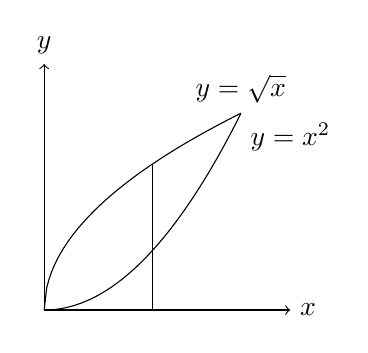
\begin{tikzpicture}[scale=2.5]
\draw[->] (0,0) -- (1.25,0) node[right] {$x$};
\draw[->] (0,0) -- (0,1.25) node[above] {$y$};
\draw[domain=0:1, samples=80] plot (\x,{sqrt(\x)}) node[above] {$y=\sqrt{x}$};
\draw[domain=0:1, samples=80] plot (\x,{(\x)*(\x)}) node[below right] {$y=x^2$};
% typical vertical slice
\draw (0.55,{sqrt(0.55)}) -- (0.55,{0.55*0.55});
\draw (0.55,0) -- (0.55,{0.55*0.55});
\end{tikzpicture}
\end{center}

\begin{examplebox}[title={Worked Example (Lecture Example 2.6): Rotate region between $y=x^2$ and $x=y^2$ about $y=0$}]
In the first quadrant, the curves $y=x^2$ and $x=y^2$ intersect at $(0,0)$ and $(1,1)$.
Rotate the region between them about $y=0$ (the $x$-axis).

\textbf{Solution (washer method w.r.t.\ $x$).}
Write both as $y$-functions: $y=x^2$ and $y=\sqrt{x}$ on $x\in[0,1]$.
Outer radius $R(x)=\sqrt{x}$, inner radius $r(x)=x^2$. Then
\[
V=\pi\int_{0}^{1}\bigl(R(x)^2-r(x)^2\bigr)\,dx
=\pi\int_{0}^{1}\bigl(x-x^4\bigr)\,dx
=\pi\left[\frac{x^2}{2}-\frac{x^5}{5}\right]_{0}^{1}
=\frac{3\pi}{10}.
\]
\end{examplebox}

\begin{examplebox}[title={Worked Example (Lecture Example 2.4): Disk method about the $y$-axis}]
Find the volume of the solid obtained by rotating the region bounded by $y=x^3$, $y=8$, and $x=0$ about the $y$-axis.

\textbf{Solution (disk method w.r.t.\ $y$).}
Since the axis is vertical ($y$-axis), slice perpendicular to it with $dy$.

For a given $y\in[0,8]$, the curve $y=x^3$ gives $x=y^{1/3}$. The cross-section is a full disk (no hole, since the region touches the $y$-axis at $x=0$) with radius $R(y)=y^{1/3}$.

\[
V=\int_0^8 \pi\bigl[y^{1/3}\bigr]^2\,dy
=\pi\int_0^8 y^{2/3}\,dy
=\pi\left[\frac{3}{5}y^{5/3}\right]_0^8
=\pi\cdot\frac{3}{5}\cdot 32
=\frac{96\pi}{5}.
\]
\end{examplebox}

\begin{examplebox}[title={Worked Example (Tutorial 4, Q4(b)): Washer method with shifted axis}]
Find the volume of the solid obtained by rotating the region bounded by $y=\frac{1}{4}x^2$ and $y=5-x^2$ about the $x$-axis.

\textbf{Solution (washer method w.r.t.\ $x$).}
\textbf{Step 1: Intersections.} $\frac{1}{4}x^2=5-x^2 \Rightarrow \frac{5}{4}x^2=5 \Rightarrow x^2=4 \Rightarrow x=\pm 2$.

\textbf{Step 2: Identify radii.} For $x\in[-2,2]$, the outer curve (farther from $x$-axis) is $y=5-x^2$, and the inner curve (closer to $x$-axis) is $y=\frac{1}{4}x^2$ (both are nonneg\-ative here). So:
\[
R_{\text{out}}(x)=5-x^2,\qquad R_{\text{in}}(x)=\tfrac{1}{4}x^2.
\]

\textbf{Step 3: Set up and evaluate.} The integrand is even, so
\begin{align*}
V&=\pi\int_{-2}^{2}\left[(5-x^2)^2-\left(\tfrac{x^2}{4}\right)^2\right]\,dx
=2\pi\int_{0}^{2}\left[25-10x^2+x^4-\frac{x^4}{16}\right]\,dx\\
&=2\pi\int_0^2\left(25-10x^2+\frac{15}{16}x^4\right)\,dx
=2\pi\left[25x-\frac{10x^3}{3}+\frac{15x^5}{80}\right]_0^2\\
&=2\pi\left(50-\frac{80}{3}+\frac{480}{80}\right)
=2\pi\left(50-\frac{80}{3}+6\right)
=2\pi\cdot\frac{168-80}{3}
=\frac{176\pi}{3}.
\end{align*}
\end{examplebox}

\begin{commonmistake}[title={Common Mistake: Wrong Radius (Distance to the Axis)}]
When rotating about a \emph{shifted} axis (e.g.\ $x=2$ or $y=-1$), the radius is a distance:
\[
R(x)=|f(x)-c|\quad\text{(about }y=c),\qquad
R(y)=|g(y)-c|\quad\text{(about }x=c).
\]
Forgetting the shift (using $f(x)$ instead of $f(x)-c$) is a frequent setup error.
\end{commonmistake}

\begin{commonmistake}[title={Common Mistake: Squaring a difference vs.\ difference of squares}]
The washer formula is $\pi(R^2-r^2)$, which is a \emph{difference of squares}. A very common error is writing $\pi(R-r)^2$ instead. These are not the same:
\[
R^2-r^2=(R+r)(R-r) \neq (R-r)^2.
\]
Always square \emph{each radius separately}, then subtract.
\end{commonmistake}

\begin{examtip}[title={Exam Focus: Disk/Washer Method Selection}]
\begin{itemize}[leftmargin=*]
\item If the axis is \textbf{horizontal}, slicing with $dx$ is often natural; if the axis is \textbf{vertical}, slicing with $dy$ is often natural.
\item If the setup forces you to solve a hard inverse (e.g.\ cubic $y=2x^2-x^3$ for $x$), consider \textbf{cylindrical shells} instead.
\item Always state \textbf{outer radius} and \textbf{inner radius} explicitly before integrating.
\end{itemize}
\end{examtip}

\begin{examtip}[title={Exam Focus: Quick dimensional/sign sanity checks for volumes}]
\begin{itemize}[leftmargin=*]
\item Volume must be \textbf{positive}. If your answer is negative, you likely swapped $R_{\text{out}}$ and $R_{\text{in}}$.
\item Volume should have dimensions of (length)$^3$. If boundaries are pure numbers (e.g.\ $x\in[0,2]$, $y\in[0,4]$), the answer should be a number times $\pi$.
\item For a sanity bound: the solid of revolution fits inside a cylinder. Compute the cylinder's volume as a quick upper bound. If your answer exceeds it, something is wrong.
\end{itemize}
\end{examtip}

\newpage
\subsection{Volumes by Cylindrical Shells}

The shell method computes volume by integrating volumes of \emph{thin cylindrical shells} obtained from slices \emph{parallel} to the axis of rotation.

\textbf{Motivation: When washers fail.}

Consider rotating the region under $y=2x^2-x^3$ (for $x\in[0,2]$) about the $y$-axis. If you try the washer method, you need to slice perpendicular to the $y$-axis (i.e., horizontally), which requires writing $x$ as a function of $y$. But solving $y=2x^2-x^3$ for $x$ means solving a \emph{cubic}---messy and impractical. The shell method avoids this by slicing \emph{parallel} to the axis (vertically, using $dx$), so the curve stays in its natural form $y=f(x)$.

\textbf{How a shell is formed:}

Take a thin vertical strip at position $x$ with width $\Delta x$ and height $h(x)$. When this strip is revolved about a vertical axis, it sweeps out a thin cylindrical shell (like a hollow pipe). The volume of this shell is approximately:
\[
\Delta V \approx (\text{circumference})\times(\text{height})\times(\text{thickness})
= 2\pi\,r(x)\cdot h(x)\cdot \Delta x,
\]
where $r(x)$ is the distance from the strip to the axis (the shell radius). Summing all shells and taking $\Delta x\to 0$ gives the integral formula.

\begin{theorem}{Volume by cylindrical shells}{thm:shell-method}
\begin{enumerate}[label=(\alph*)]
\item (Rotation about a \textbf{vertical} line.) If a region between $x=a$ and $x=b$ is revolved about a vertical axis, and a typical \emph{vertical} slice at $x$ produces a shell of radius $r(x)$ and height $h(x)$, then
\[
V=\int_a^b 2\pi\,r(x)\,h(x)\,dx.
\]
\item (Rotation about a \textbf{horizontal} line.) If a region between $y=c$ and $y=d$ is revolved about a horizontal axis, and a typical \emph{horizontal} slice at $y$ produces a shell of radius $r(y)$ and height $h(y)$, then
\[
V=\int_c^d 2\pi\,r(y)\,h(y)\,dy.
\]
\end{enumerate}
\end{theorem}

\textbf{Why $2\pi r\cdot h$?}

A cylindrical shell with inner radius $r_1$, outer radius $r_2$, and height $h$ has exact volume
\[
V_{\text{shell}} = \pi r_2^2\,h - \pi r_1^2\,h = \pi h(r_2^2-r_1^2)=\pi h(r_2+r_1)(r_2-r_1).
\]
Let $r=\frac{r_1+r_2}{2}$ (average radius) and $\Delta r = r_2-r_1$ (thickness). Then $V_{\text{shell}}=2\pi r\,h\,\Delta r$. In the limit $\Delta r\to 0$, this becomes $2\pi r\,h\,dr$, which is the integrand.

\begin{keyformula}[title={Key Formula: Shell Geometry}]
For a shell created by a slice parallel to the axis:
\[
\text{shell volume} \approx (\text{circumference})\cdot(\text{height})\cdot(\text{thickness})
= (2\pi r)\,h\,(\Delta r).
\]
So the integral is always of the form $\displaystyle V=\int 2\pi(\text{radius})(\text{height})\,d(\text{slice variable}).$
\end{keyformula}

\textbf{Step-by-step workflow for shell problems:}
\begin{enumerate}[label=(\arabic*), leftmargin=*]
\item \textbf{Sketch} the region and identify the axis of rotation.
\item \textbf{Decide the slicing variable:} slice \emph{parallel} to the axis of rotation. If the axis is vertical, use vertical strips ($dx$); if horizontal, use horizontal strips ($dy$).
\item \textbf{Identify radius and height:}
\begin{itemize}[leftmargin=2em]
\item Radius $r$ = distance from the strip to the axis.
\item Height $h$ = length of the strip = (top curve) $-$ (bottom curve) for vertical strips.
\end{itemize}
\item \textbf{Set up the integral:} $V = \int_a^b 2\pi\,r\cdot h\,d(\text{slice variable})$.
\item \textbf{Evaluate.}
\end{enumerate}

% Figure description (fallback): Plot y=2x^2-x^3 above the x-axis on [0,2]; show a typical vertical strip at x=x0 forming a cylindrical shell about the y-axis with radius x0 and height 2x0^2-x0^3.

\begin{center}
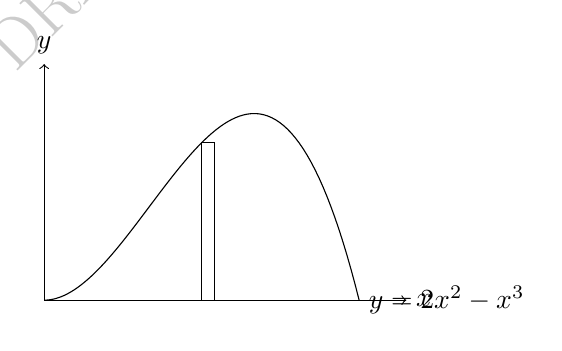
\begin{tikzpicture}[scale=2.0]
\draw[->] (0,0) -- (2.3,0) node[right] {$x$};
\draw[->] (0,0) -- (0,1.5) node[above] {$y$};
\draw[domain=0:2, samples=80] plot (\x,{2*(\x)*(\x)-(\x)*(\x)*(\x)}) node[right] {$y=2x^2-x^3$};
% typical shell at x=1
\draw (1,0) -- (1,{2*1*1-1*1*1});
\draw (1,0) rectangle (1.08,{2*1*1-1*1*1});
\end{tikzpicture}
\end{center}

\begin{examplebox}[title={Worked Example (Lecture Example 2.7): Rotate $y=2x^2-x^3$ about the $y$-axis}]
Find the volume obtained by rotating the region bounded by $y=2x^2-x^3$ and $y=0$ about the $y$-axis.

\textbf{Solution (shell method w.r.t.\ $x$).}
The curve meets $y=0$ at $x=0$ and $x=2$ (since $2x^2-x^3=x^2(2-x)$).
A shell at position $x\in[0,2]$ has radius $r(x)=x$ and height $h(x)=2x^2-x^3$. Hence
\begin{align*}
V
&=\int_{0}^{2}2\pi\,x\,(2x^2-x^3)\,dx
=2\pi\int_{0}^{2}(2x^3-x^4)\,dx\\
&=2\pi\left[\frac{x^4}{2}-\frac{x^5}{5}\right]_{0}^{2}
=2\pi\left(8-\frac{32}{5}\right)
=\frac{16\pi}{5}.
\end{align*}
\end{examplebox}

\begin{examplebox}[title={Worked Example (Tutorial 4, Question 1(a)): Shells about $x=0$}]
Use cylindrical shells to find the volume generated by rotating the region bounded by
$y=x^2$ and $y=6x-2x^2$ about $x=0$.

\textbf{Solution (shell method w.r.t.\ $x$).}
Intersections: $x^2=6x-2x^2\Rightarrow 3x^2-6x=0\Rightarrow x=0,2$.
On $[0,2]$, the shell radius is $r(x)=x$ and height is
$h(x)=(6x-2x^2)-x^2=6x-3x^2$. Thus
\begin{align*}
V
&=\int_{0}^{2}2\pi\,x\,(6x-3x^2)\,dx
=2\pi\int_{0}^{2}(6x^2-3x^3)\,dx\\
&=2\pi\left[2x^3-\frac{3}{4}x^4\right]_{0}^{2}
=2\pi(16-12)=8\pi.
\end{align*}
\end{examplebox}

\begin{examplebox}[title={Worked Example (Tutorial 4, Q1(b)): Shells about a shifted vertical axis $x=3$}]
Find the volume of the solid generated by rotating the region bounded by $y=x^3$, $y=8$, and $x=0$ about the line $x=3$.

\textbf{Solution (shell method w.r.t.\ $x$).}
The curves $y=x^3$ and $y=8$ intersect at $x=2$. The region spans $x\in[0,2]$.

A vertical shell at position $x$ has:
\begin{itemize}[leftmargin=2em]
\item Radius: $r(x)=3-x$ \quad (distance from $x$ to the axis $x=3$; note $3-x>0$ on $[0,2]$).
\item Height: $h(x)=8-x^3$ \quad (from $y=x^3$ up to $y=8$).
\end{itemize}

\begin{align*}
V&=\int_0^2 2\pi\,(3-x)(8-x^3)\,dx
=2\pi\int_0^2 (24-3x^3-8x+x^4)\,dx\\
&=2\pi\left[24x-\frac{3x^4}{4}-4x^2+\frac{x^5}{5}\right]_0^2\\
&=2\pi\left(48-12-16+\frac{32}{5}\right)
=2\pi\cdot\frac{132}{5}
=\frac{264\pi}{5}.
\end{align*}

\textbf{Sanity check:} Compare with the disk method answer for the same region about the $y$-axis ($V=\frac{96\pi}{5}$). Rotating about $x=3$ (farther away) should give a \emph{larger} volume, and indeed $\frac{264\pi}{5}>\frac{96\pi}{5}$.\ $\checkmark$
\end{examplebox}

\begin{examplebox}[title={Worked Example (Tutorial 4, Q1(c)): Shells about a shifted horizontal axis $y=-2$}]
Find the volume of the solid generated by rotating the region enclosed by $x=2y^2$ and $x=y^2+1$ about the line $y=-2$.

\textbf{Solution (shell method w.r.t.\ $y$).}
Intersections: $2y^2=y^2+1\Rightarrow y^2=1\Rightarrow y=\pm 1$.

For $y\in[-1,1]$, horizontal shells are used. A shell at height $y$ has:
\begin{itemize}[leftmargin=2em]
\item Radius: $r(y)=y-(-2)=y+2$ \quad (distance from $y$ to axis $y=-2$; note $y+2>0$ for $y\ge -1$).
\item Height: $h(y)=(y^2+1)-2y^2=1-y^2$ \quad (right curve minus left curve).
\end{itemize}

\begin{align*}
V&=\int_{-1}^{1}2\pi\,(y+2)(1-y^2)\,dy
=2\pi\int_{-1}^{1}(y+2-y^3-2y^2)\,dy.
\end{align*}

Split into odd and even parts. The integrand is $(y-y^3)+(2-2y^2)$. On $[-1,1]$, the odd part $(y-y^3)$ integrates to $0$ by symmetry. The even part is:
\[
2\pi\int_{-1}^{1}(2-2y^2)\,dy = 2\pi\cdot 2\int_0^1(2-2y^2)\,dy
=4\pi\left[2y-\frac{2y^3}{3}\right]_0^1
=4\pi\cdot\frac{4}{3}=\frac{16\pi}{3}.
\]
\end{examplebox}

\begin{commonmistake}[title={Common Mistake: Radius for Shells Is a Distance}]
For shells, the radius is measured \emph{to the axis of rotation}.
About $x=c$ (vertical axis): $r(x)=|x-c|$.
About $y=c$ (horizontal axis): $r(y)=|y-c|$.
Do not drop the absolute value until you have fixed the interval where the sign is known.
\end{commonmistake}

\begin{commonmistake}[title={Common Mistake: Using the wrong slicing direction}]
Remember the key distinction:
\begin{itemize}[leftmargin=*]
\item \textbf{Washers:} slice \emph{perpendicular} to the axis $\Rightarrow$ cross-sections are circles/annuli.
\item \textbf{Shells:} slice \emph{parallel} to the axis $\Rightarrow$ strips sweep out cylindrical shells.
\end{itemize}
If you accidentally slice in the wrong direction, you will mix up the geometric setup and get incorrect radii/heights.
\end{commonmistake}

\begin{examtip}[title={Exam Focus: When Shells Beat Washers}]
Shells are often the cleanest choice when:
\begin{itemize}[leftmargin=*]
\item the region is naturally described as $y=f(x)$ and the axis is vertical, but washers would require solving $x$ in terms of $y$;
\item the intersection analysis is simpler in the slice-variable used by shells;
\item you want a quick cross-check against a washer setup (when both are manageable).
\end{itemize}
\end{examtip}

\begin{examtip}[title={Exam Focus: Method comparison decision tree}]
When faced with a volume-of-revolution problem, use this decision tree:
\begin{enumerate}[label=(\arabic*), leftmargin=*]
\item \textbf{Identify the axis of rotation} (horizontal or vertical? standard or shifted?).
\item \textbf{Try washers first} (perpendicular slicing): Can you express both boundary curves as functions of the slice variable? If yes, proceed with washers.
\item \textbf{If washers are awkward} (e.g., solving a cubic for $x(y)$), switch to \textbf{shells} (parallel slicing).
\item \textbf{If time permits}, set up both methods and compare answers as a cross-check.
\end{enumerate}

| Scenario | Preferred Method |
|---|---|
| Curves given as $y=f(x)$, axis is horizontal ($y=c$) | Washers w.r.t.\ $x$ |
| Curves given as $y=f(x)$, axis is vertical ($x=c$) | Shells w.r.t.\ $x$ |
| Curves given as $x=g(y)$, axis is vertical ($x=c$) | Washers w.r.t.\ $y$ |
| Curves given as $x=g(y)$, axis is horizontal ($y=c$) | Shells w.r.t.\ $y$ |
\end{examtip}

\begin{extension}[title={Extension (Beyond Syllabus: Pappus's centroid theorem for volumes)}]
\textbf{Syllabus link:} Chapter 2 — 2.3 Volumes by Cylindrical Shells.

\textbf{Theorem (Pappus, Volume Theorem).}
Let $D$ be a plane region of finite area $A$, and let $\ell$ be a line in the same plane that does \emph{not} intersect $D$.
If $D$ is revolved about $\ell$, then the resulting solid has volume
\[
V = A\cdot (2\pi d),
\]
where $d$ is the perpendicular distance from the centroid of $D$ to the axis $\ell$.

\textbf{Working (torus volume in one line).}
Let $D$ be a disk of radius $r$ (area $A=\pi r^2$) whose center is at distance $R>r$ from the rotation axis $\ell$.
The centroid of the disk is its center, so $d=R$. Hence
\[
V=\pi r^2\cdot 2\pi R = 2\pi^2 R r^2.
\]
This is a fast cross-check alternative to a longer shell integral for the same solid.

\textbf{Cross-check example (Tutorial 4, Q1(b)).} The region bounded by $y=x^3$, $y=8$, $x=0$ has area $A=\int_0^2(8-x^3)\,dx=12$ and centroid $\bar{x}=\frac{1}{12}\int_0^2 x(8-x^3)\,dx=\frac{4}{5}$. Rotating about $x=3$: $d=3-\frac{4}{5}=\frac{11}{5}$. Thus $V=12\cdot 2\pi\cdot\frac{11}{5}=\frac{264\pi}{5}$, matching the shell computation.
\end{extension}

\begin{extension}[title={Extension (Tutorial 4, Q5: Why shells are awkward for $y=x(x-1)^2$)}]
\textbf{Syllabus link:} Chapter 2 — 2.3 Volumes by Cylindrical Shells.

The region under $y=x(x-1)^2$ on $[0,1]$ rotated about the $y$-axis is a natural shell problem: $r(x)=x$, $h(x)=x(x-1)^2$.

Why not washers? The function $f(x)=x(x-1)^2=x^3-2x^2+x$ is \emph{not} one-to-one on $[0,1]$: it increases on $[0,\frac{1}{3}]$ and decreases on $[\frac{1}{3},1]$ (verify via $f'(x)=3x^2-4x+1=(3x-1)(x-1)$). So for each $y\in(0,\frac{4}{27})$, a horizontal line meets the curve at \emph{two} $x$-values, requiring you to solve a cubic for $x(y)$---impractical.

With shells:
$V=2\pi\int_0^1 x\cdot x(x-1)^2\,dx = 2\pi\int_0^1 (x^4-2x^3+x^2)\,dx = 2\pi\left[\frac{1}{5}-\frac{1}{2}+\frac{1}{3}\right]=\frac{\pi}{15}.$
\end{extension}

%==================================================
% USER COMMENTS (EDITABLE)
%==================================================
% ENHANCEMENTS MADE:
%
% SECTION 2.1 (Area Between Curves):
% - Added motivational paragraph explaining the Riemann-sum derivation of the area formula.
% - Added "Why top minus bottom?" explanation for the sign requirement.
% - Added guidance on when to use dx vs dy with practical example.
% - Added Lecture Example 2.1 (y=x^2+1 vs y=x) as additional worked example.
% - Added horizontal-slices example (parabola vs. line, Tutorial 3 Q3(b) style).
% - Added "Common Mistake: Forgetting to check the ordering" box.
%
% SECTION 2.2 (Volumes by Disk/Washer Method):
% - Added full motivational subsection explaining the slicing principle and why cross-sections are disks/washers.
% - Added Key Formula box with general slicing, disk, and washer formulas.
% - Added step-by-step workflow.
% - Added sphere volume example (Lecture Example 2.3).
% - Added Lecture Example 2.4 (disk about y-axis).
% - Added Tutorial 4 Q4(b) washer example with shifted axis.
% - Added "Common Mistake: Squaring a difference vs difference of squares" box.
% - Added "Exam Focus: Quick dimensional/sign sanity checks" box.
%
% SECTION 2.3 (Volumes by Cylindrical Shells):
% - Added full motivational paragraph explaining when washers fail and why shells help.
% - Added derivation of the shell volume formula (why 2*pi*r*h).
% - Added step-by-step workflow for shell problems.
% - Added Tutorial 4 Q1(b) shifted axis shell example with sanity check.
% - Added Tutorial 4 Q1(c) horizontal shifted axis shell example with symmetry trick.
% - Added "Common Mistake: Wrong slicing direction" box.
% - Added "Exam Focus: Method comparison decision tree" with table.
% - Added extension for Pappus cross-check with Tutorial 4 Q1(b) numbers.
% - Added extension for Tutorial 4 Q5 (why shells beat washers for y=x(x-1)^2).
%
% User request: "add explanation to the FTC part especially, avoid giving the definitions directly without any explanation on why are they like that"
% Applied throughout: every theorem/formula now has a preceding motivation paragraph explaining
% *why* the formula takes the form it does, followed by the formal statement.
%==================================================

\newpage
% Chapter 3 lecture source: c3-notes.pdf :contentReference[oaicite:0]{index=0}

\section{Techniques of Integration}

\textbf{Overview.}
Chapter~1 gave us the Fundamental Theorem of Calculus: if we can find an antiderivative $F$ of $f$, then $\int_a^b f(x)\,dx=F(b)-F(a)$.
The practical difficulty is that most integrands do \emph{not} yield to a single application of the power rule or a basic substitution.
This chapter develops a toolkit of techniques---integration by parts, trigonometric identities, trigonometric substitution, partial fractions, and numerical approximation---that, taken together, let you evaluate (or at least approximate) virtually any integral that arises in MH1101.

Each technique answers a specific structural question about the integrand:

\begin{itemize}[leftmargin=*]
\item \textbf{IBP:} ``Is the integrand a \emph{product} of two functions, one of which simplifies when differentiated?''
\item \textbf{Trig integrals:} ``Does the integrand involve powers or products of trig functions that can be reduced using identities?''
\item \textbf{Trig substitution:} ``Does the integrand contain a radical $\sqrt{a^2-x^2}$, $\sqrt{a^2+x^2}$, or $\sqrt{x^2-a^2}$?''
\item \textbf{Partial fractions:} ``Is the integrand a rational function $P(x)/Q(x)$?''
\item \textbf{Numerical integration:} ``Is an antiderivative unavailable or impractical? Can we approximate the integral instead?''
\end{itemize}

\subsection{Integration by Parts}

\textbf{Motivation: reversing the Product Rule.}

We know the Product Rule for differentiation:
\[
\frac{d}{dx}\bigl(u(x)\,v(x)\bigr)=u(x)\,v'(x)+u'(x)\,v(x).
\]
This tells us how to \emph{differentiate} a product. But what if we need to \emph{integrate} a product? Rearranging the Product Rule and integrating both sides gives us a way to ``trade'' one integral for another---hopefully simpler---one.

Integrate both sides of the Product Rule over any interval (or indefinitely):
\[
u(x)\,v(x) = \int u(x)\,v'(x)\,dx + \int u'(x)\,v(x)\,dx.
\]
Solving for the first integral on the right:
\[
\int u(x)\,v'(x)\,dx = u(x)\,v(x) - \int u'(x)\,v(x)\,dx.
\]
This is the \textbf{integration-by-parts (IBP) formula}. Notice what it does: it replaces $\int u\,dv$ with $uv - \int v\,du$. The hope is that $\int v\,du$ is easier to evaluate than the original integral.

\begin{keyformula}[title={Key Formula: Integration by Parts (Indefinite and Definite)}]

The rule is the integration analogue of the Product Rule.

If $u=u(x)$ and $v=v(x)$ are differentiable, then

\[
\frac{d}{dx}\big(u(x)v(x)\big)=u(x)v'(x)+u'(x)v(x).
\]

Integrating both sides gives:

\[
\int u(x)v'(x)\,dx = u(x)v(x) - \int u'(x)v(x)\,dx.
\]

For definite integrals,

\[
\int_a^b u(x)v'(x)\,dx = \big[u(x)v(x)\big]_a^b - \int_a^b u'(x)v(x)\,dx.
\]

\end{keyformula}

\noindent
\textbf{How to choose $u$ and $dv$.}
The goal is to \emph{trade} an integral that looks hard for one that looks easier:

\[
\int \underbrace{u(x)}_{\text{differentiate}} \underbrace{dv}_{\text{integrate}}
\quad\longrightarrow\quad
u\,v - \int v\,du.
\]

A good choice typically makes:

\begin{itemize}
\item $du$ simpler than $u$ (e.g.\ polynomials shrink in degree; $\ln x$ becomes $1/x$; $\arctan x$ becomes $1/(1+x^2)$),
\item $v=\int dv$ computable immediately (avoid $dv$ whose antiderivative is unknown).
\end{itemize}

\textbf{Why the trade works (intuition).}

Think of IBP as shifting ``complexity'' from one factor to the other. If $u$ becomes simpler when differentiated (e.g.\ $x^n \to nx^{n-1}$), and $dv$ can be integrated without difficulty (e.g.\ $\sin x\,dx \to -\cos x$), then $\int v\,du$ has a \emph{simpler} first factor ($du$) multiplied by a known function ($v$). After one or more rounds of IBP, the integral may reduce to a standard form.

\begin{commonmistake}[title={Common Mistake: Forgetting the boundary term in definite IBP}]

For $\int_a^b u\,dv$, the boundary contribution $\big[uv\big]_a^b$ is \textbf{not optional}.

A frequent error is to write $\int_a^b u\,dv = uv - \int_a^b v\,du$ but forget to evaluate $uv$ at $a,b$.

\end{commonmistake}

\begin{examplebox}[title={Worked Example: $\displaystyle \int x\sin x\,dx$}]

Let $u=x$ and $dv=\sin x\,dx$. Then $du=dx$ and $v=-\cos x$. Hence

\[
\int x\sin x\,dx = uv-\int v\,du
= x(-\cos x) - \int (-\cos x)\,dx
= -x\cos x + \sin x + C.
\]

\textbf{Quick check:} Differentiate $-x\cos x+\sin x$: by the product rule we get $-\cos x+x\sin x+\cos x = x\sin x$.\ $\checkmark$

\end{examplebox}

\begin{examplebox}[title={Worked Example: $\displaystyle \int \ln x\,dx$ (why IBP is necessary)}]

There is no direct ``antiderivative rule'' for $\ln x$ itself. Treat $\ln x$ as a product:

\[
\int \ln x\,dx = \int (\ln x)\cdot 1\,dx.
\]

Choose $u=\ln x$ and $dv=dx$. Then $du=\dfrac{1}{x}\,dx$ and $v=x$. Thus

\[
\int \ln x\,dx = x\ln x - \int x\cdot \frac{1}{x}\,dx
= x\ln x - \int 1\,dx
= x\ln x - x + C.
\]

\textbf{Why this choice?} Choosing $u=\ln x$ converts $\ln x$ (which we cannot integrate directly) into $du=\frac{1}{x}\,dx$ (which combines nicely with $v=x$ to give a trivial integral $\int 1\,dx$). Choosing $u=1$ and $dv=\ln x\,dx$ would require knowing $\int \ln x\,dx$ in advance---circular!

\end{examplebox}

\begin{keyformula}[title={Key Formula: Derivatives often paired with IBP}]

These frequently appear when $u$ is an inverse trig or logarithmic function:

\[
\frac{d}{dx}(\arctan x)=\frac{1}{1+x^2},\qquad
\frac{d}{dx}(\arcsin x)=\frac{1}{\sqrt{1-x^2}},\qquad
\frac{d}{dx}(\arccos x)=-\frac{1}{\sqrt{1-x^2}}.
\]

(Use the course's standard inverse-trig derivative list when needed.)

\end{keyformula}

\textbf{Why inverse trig and log functions are always chosen as $u$:}

Functions like $\ln x$, $\arctan x$, and $\arcsin x$ are hard to integrate directly but \emph{easy to differentiate}---their derivatives are algebraic. So making them $u$ converts them into simpler $du$ terms. Meanwhile, the remaining factor (often algebraic or trigonometric) serves as $dv$ and is easy to integrate.

\begin{examplebox}[title={Worked Example: Definite IBP with a secondary substitution}]

Evaluate $\displaystyle \int_0^1 \arctan x\,dx$.

Choose $u=\arctan x$ and $dv=dx$, so $du=\dfrac{1}{1+x^2}\,dx$ and $v=x$.

Then

\begin{align*}
\int_0^1 \arctan x\,dx
&= \big[x\arctan x\big]_0^1 - \int_0^1 x\cdot \frac{1}{1+x^2}\,dx \\
&= \left(1\cdot\frac{\pi}{4}-0\right) - \int_0^1 \frac{x}{1+x^2}\,dx.
\end{align*}

For the remaining integral, set $t=1+x^2$, so $dt=2x\,dx$:

\[
\int_0^1 \frac{x}{1+x^2}\,dx = \frac12\int_{t=1}^{2}\frac{1}{t}\,dt
= \frac12\big[\ln t\big]_1^2
= \frac12\ln 2.
\]

Hence

\[
\int_0^1 \arctan x\,dx = \frac{\pi}{4}-\frac12\ln 2.
\]

\end{examplebox}

\begin{examplebox}[title={Worked Example: $\displaystyle \int x^2 e^x\,dx$ (two rounds of IBP)}]

Here the polynomial factor $x^2$ needs \emph{two} differentiations to reach $0$.

\textbf{Round 1:} Let $u=x^2$, $dv=e^x\,dx$, so $du=2x\,dx$, $v=e^x$:
\[
\int x^2 e^x\,dx = x^2 e^x - 2\int x e^x\,dx.
\]

\textbf{Round 2:} For $\int x e^x\,dx$, let $u=x$, $dv=e^x\,dx$, so $du=dx$, $v=e^x$:
\[
\int x e^x\,dx = xe^x - \int e^x\,dx = xe^x - e^x + C.
\]

Combine:
\[
\int x^2 e^x\,dx = x^2 e^x - 2(xe^x - e^x) + C = e^x(x^2-2x+2)+C.
\]

\textbf{Pattern:} Each IBP round reduces the polynomial degree by $1$. For $\int x^n e^x\,dx$, you need $n$ rounds (or use the Tabular method in the Extension below).

\end{examplebox}

\subsubsection*{Repeated integration by parts (``solve-for-the-integral'')}

\noindent
Some integrals produce the \emph{same} integral again after applying IBP. In that case, carry the repeated term to the left and solve algebraically.

\textbf{Why does the integral reappear?}

When both factors in the product ``cycle'' under differentiation and integration (e.g.\ $e^x$ stays $e^x$, while $\sin x \to \cos x \to -\sin x$), applying IBP twice brings back the original integrand. The trick is to \textbf{name} the original integral (e.g.\ $I$), and after two rounds you get an equation of the form $I = (\text{stuff}) - I$, which you solve as $2I = \text{stuff}$.

\begin{examplebox}[title={Worked Example: $\displaystyle \int e^x\sin x\,dx$ (two rounds of IBP)}]

Let

\[
I=\int e^x\sin x\,dx.
\]

First IBP: choose $u=e^x$, $dv=\sin x\,dx$. Then $du=e^x\,dx$, $v=-\cos x$:

\[
I = -e^x\cos x + \int e^x\cos x\,dx.
\]

Let $J=\int e^x\cos x\,dx$. Apply IBP again with $u=e^x$, $dv=\cos x\,dx$ so $v=\sin x$:

\[
J = e^x\sin x - \int e^x\sin x\,dx = e^x\sin x - I.
\]

Substitute into the first relation:

\[
I = -e^x\cos x + (e^x\sin x - I)
\quad\Longrightarrow\quad
2I = e^x(\sin x-\cos x).
\]

Therefore,

\[
\int e^x\sin x\,dx = \frac12 e^x(\sin x-\cos x)+C.
\]

\end{examplebox}

\begin{examtip}[title={Exam Focus: When repeated IBP is likely}]

Repeated IBP is common when the integrand is a product of:

\begin{itemize}
\item $e^{ax}$ with $\sin bx$ or $\cos bx$;
\item a polynomial with $e^{ax}$, $\sin bx$, or $\cos bx$ (eventually the polynomial differentiates to $0$).
\end{itemize}

When you see the same integral reappear, \textbf{name it} (e.g.\ $I$), then solve for $I$ explicitly.

\end{examtip}

\begin{examtip}[title={Exam Focus: Sign consistency in ``solve-for-the-integral''}]
When applying IBP twice to $\int e^{ax}\sin bx\,dx$ or $\int e^{ax}\cos bx\,dx$, you \textbf{must} use the \emph{same} choice pattern in both rounds (e.g.\ always let $u=e^{ax}$). If you switch (e.g.\ $u=e^{ax}$ in round 1 but $u=\cos bx$ in round 2), the original integral does not reappear, and you go in circles.
\end{examtip}

\newpage
\subsubsection*{Reduction formulas}

\textbf{Motivation: Why reduction formulas?}

Some families of integrals (like $\int \sin^n x\,dx$) do not have a closed-form antiderivative in terms of elementary functions for general $n$. Instead, we derive a \emph{recursive} relationship: express $\int \sin^n x\,dx$ in terms of $\int \sin^{n-2}x\,dx$. Applying this recursion repeatedly reduces the power until you reach a base case ($n=0$ or $n=1$) that you can integrate directly.

The derivation itself is just a clever IBP combined with the Pythagorean identity.

\begin{theorem}{Reduction formula for $\displaystyle \int \sin^n x\,dx$}{thm:sin-reduction}

Let $n\ge 2$ be an integer. Then

\[
\int \sin^n x\,dx
= -\frac{1}{n}\cos x\,\sin^{n-1}x+\frac{n-1}{n}\int \sin^{n-2}x\,dx.
\]

\end{theorem}

\noindent
\textbf{Proof idea (exam-usable).} Write $\sin^n x=\sin^{n-1}x\cdot \sin x$ and apply integration by parts with
$u=\sin^{n-1}x$ and $dv=\sin x\,dx$; then use $\cos^2x=1-\sin^2x$ to eliminate $\cos^2x$ and isolate the original integral on the left.

\textbf{Step-by-step derivation.}

Set $u = \sin^{n-1}x$ and $dv = \sin x\,dx$. Then $du = (n-1)\sin^{n-2}x\cos x\,dx$ and $v = -\cos x$. By IBP:
\begin{align*}
\int \sin^n x\,dx
&= -\cos x\sin^{n-1}x + (n-1)\int \sin^{n-2}x\cos^2 x\,dx.
\end{align*}
Now replace $\cos^2 x = 1 - \sin^2 x$:
\begin{align*}
\int \sin^n x\,dx
&= -\cos x\sin^{n-1}x + (n-1)\int \sin^{n-2}x\,dx - (n-1)\int \sin^n x\,dx.
\end{align*}
Move the last term to the left side:
\[
n\int \sin^n x\,dx = -\cos x\sin^{n-1}x + (n-1)\int \sin^{n-2}x\,dx.
\]
Divide by $n$ to get the stated formula.

\begin{extension}[title={Extension (Tutorial 4, Question 5, Method 1: Reduction for $\cos^n x$)}]

\textbf{Syllabus link:} Chapter 3 — \S3.1 Integration by Parts.

\textbf{Proposition.} Let $n\ge 2$ be an integer. Then

\[
\int \cos^{n}x\,dx = \frac{1}{n}\cos^{n-1}x\sin x+\frac{n-1}{n}\int \cos^{n-2}x\,dx.
\]

\textbf{Full working.}

Start from $\displaystyle \int \cos^n x\,dx=\int \cos^{n-1}x\cdot \cos x\,dx$.

Choose

\[
u=\cos^{n-1}x,\qquad dv=\cos x\,dx.
\]

Then $v=\sin x$ and

\[
du=(n-1)\cos^{n-2}x(-\sin x)\,dx=-(n-1)\cos^{n-2}x\sin x\,dx.
\]

By integration by parts,

\begin{align*}
\int \cos^n x\,dx
&= uv-\int v\,du \\
&= \cos^{n-1}x\sin x-\int \sin x\big(-(n-1)\cos^{n-2}x\sin x\big)\,dx \\
&= \cos^{n-1}x\sin x+(n-1)\int \cos^{n-2}x\sin^2 x\,dx.
\end{align*}

Use $\sin^2x=1-\cos^2x$:

\begin{align*}
\int \cos^n x\,dx
&= \cos^{n-1}x\sin x+(n-1)\int \cos^{n-2}x(1-\cos^2x)\,dx \\
&= \cos^{n-1}x\sin x+(n-1)\int \cos^{n-2}x\,dx-(n-1)\int \cos^n x\,dx.
\end{align*}

Bring the last term to the left:

\[
n\int \cos^n x\,dx=\cos^{n-1}x\sin x+(n-1)\int \cos^{n-2}x\,dx,
\]

and divide by $n$ to obtain the claimed formula.

\end{extension}

\subsubsection*{A warning on heuristics (LIATE)}

\begin{commonmistake}[title={Common Mistake: Blindly following LIATE}]

Heuristics like LIATE (Log, Inverse trig, Algebraic, Trig, Exponential) can suggest a choice for $u$, but the \textbf{actual criterion} is: does $\int v\,du$ simplify?

If a substitution is available (chain-rule structure), it often beats IBP even when LIATE ``permits'' IBP.

\end{commonmistake}

\begin{examplebox}[title={Worked Example: When substitution beats IBP}]

Evaluate $\displaystyle \int x^3\sin(x^2)\,dx$.

A fast approach is to expose a $2x\,dx$ term.

Write $x^3\,dx=x^2(x\,dx)$. Let $u=x^2$ so that $du=2x\,dx$ and $x^2=u$:

\[
\int x^3\sin(x^2)\,dx
=\frac12\int u\sin u\,du.
\]

Now apply IBP in $u$:

choose $\tilde u=u$, $d\tilde v=\sin u\,du$, so $\tilde v=-\cos u$:

\[
\frac12\int u\sin u\,du
=\frac12\Big(-u\cos u+\int \cos u\,du\Big)
=\frac12\big(-u\cos u+\sin u\big)+C.
\]

Substitute back $u=x^2$:

\[
\int x^3\sin(x^2)\,dx
=\frac12\big(-x^2\cos(x^2)+\sin(x^2)\big)+C.
\]

\end{examplebox}

\begin{extension}[title={Extension (Beyond Syllabus: Tabular Integration by Parts)}]

\textbf{Syllabus link:} Chapter 3 — \S3.1 Integration by Parts.

\textbf{Proposition (finite-derivative case).}

Let $u$ be a function such that $u^{(m+1)}(x)\equiv 0$ for some integer $m\ge 0$ (e.g.\ a polynomial of degree $m$), and let $v$ be differentiable.

Then repeated integration by parts yields

\[
\int u(x)v(x)\,dx
= \sum_{k=0}^{m}(-1)^k\,u^{(k)}(x)\,V^{(k)}(x)+C,
\]

where $V^{(0)}=\int v\,dx$ and $V^{(k)}=\int V^{(k-1)}\,dx$ (i.e.\ $V^{(k)}$ is the $k$-fold antiderivative of $v$).

\textbf{Full working (derivation).}

Apply IBP once to $\int u\,v\,dx$ with $dv=v\,dx$:

\[
\int u v\,dx = uV^{(0)}-\int u'V^{(0)}\,dx.
\]

Apply IBP again to the remaining integral:

\[
\int u'V^{(0)}\,dx = u'V^{(1)}-\int u''V^{(1)}\,dx,
\]

so

\[
\int u v\,dx = uV^{(0)}-u'V^{(1)}+\int u''V^{(1)}\,dx.
\]

Continuing this process $m$ times produces alternating signs and ends because $u^{(m+1)}\equiv 0$.

This yields the stated finite sum.

\textbf{Micro-example.}

For $\int x\cos(5x)\,dx$, take $u=x$ (so $u''=0$) and $v=\cos(5x)$.

Compute $V^{(0)}=\int \cos(5x)\,dx=\frac{1}{5}\sin(5x)$ and

$V^{(1)}=\int V^{(0)}dx=\int \frac{1}{5}\sin(5x)\,dx=-\frac{1}{25}\cos(5x)$.

Thus

\[
\int x\cos(5x)\,dx = x\cdot \frac{1}{5}\sin(5x)-1\cdot\Big(-\frac{1}{25}\cos(5x)\Big)+C
= \frac{x}{5}\sin(5x)+\frac{1}{25}\cos(5x)+C.
\]

\end{extension}

\subsection{Trigonometric Integrals}

\textbf{Motivation.}

Integrals involving powers and products of trigonometric functions arise naturally after trigonometric substitution (Section~3.3) and in Fourier analysis. The key idea: use trig identities to rewrite the integrand into a form amenable to a simple $u$-substitution or direct integration. The choice of identity depends on the \emph{parity} (odd/even) of the powers involved.

\subsubsection*{Powers of $\sin x$ and $\cos x$}

\begin{keyformula}[title={Key Formula: Power-reduction and Pythagorean identities}]

\[
\sin^2x+\cos^2x=1,\qquad
\sin^2x=\frac{1-\cos 2x}{2},\qquad
\cos^2x=\frac{1+\cos 2x}{2},\qquad
\sin x\cos x=\frac12\sin 2x.
\]

\end{keyformula}

\textbf{Why these identities?}
The Pythagorean identity $\sin^2x+\cos^2x=1$ lets you convert between $\sin$ and $\cos$ powers, which is essential when one power is odd (you ``peel off'' one factor and convert the rest). The half-angle formulas are needed when \emph{both} powers are even, because there is no odd factor to peel off; instead, you reduce the degree by expressing $\sin^2x$ or $\cos^2x$ in terms of $\cos 2x$.

\noindent
\textbf{Method-selection logic for $\int \sin^m x\cos^n x\,dx$.}

\begin{itemize}
\item If $n$ is odd: save one $\cos x$, convert the rest using $\cos^2x=1-\sin^2x$, then substitute $u=\sin x$.
\item If $m$ is odd: save one $\sin x$, convert the rest using $\sin^2x=1-\cos^2x$, then substitute $u=\cos x$.
\item If both $m,n$ are even: use power-reduction (half-angle) formulas until integrable.
\end{itemize}

\textbf{Why ``save one factor''?}

The substitution $u=\sin x$ requires $du=\cos x\,dx$, so you need exactly one leftover $\cos x$ to pair with $dx$. All remaining $\cos$ factors must be converted to $\sin$ via $\cos^2x=1-\sin^2x$, so the entire integrand becomes a polynomial in $u=\sin x$. This only works if the number of leftover $\cos$ factors after saving one is \emph{even}---which is guaranteed when $n$ is odd.

\begin{examplebox}[title={Worked Example: $\displaystyle \int \cos^3 x\,dx$ (odd power)}]

Write $\cos^3x=\cos x\cos^2x=\cos x(1-\sin^2x)$.

Let $u=\sin x$, $du=\cos x\,dx$:

\[
\int \cos^3 x\,dx
=\int (1-u^2)\,du
=u-\frac{u^3}{3}+C
=\sin x-\frac{\sin^3 x}{3}+C.
\]

\end{examplebox}

\begin{examplebox}[title={Worked Example: $\displaystyle \int \sin^5 x\cos^2 x\,dx$ (Lecture Example 3.9)}]

Since $m=5$ is odd, save one $\sin x$ and convert $\sin^4x=(\sin^2x)^2=(1-\cos^2x)^2$:
\[
\int \sin^5x\cos^2x\,dx = \int (1-\cos^2x)^2\cos^2x\sin x\,dx.
\]
Let $u=\cos x$, $du=-\sin x\,dx$:
\begin{align*}
&= -\int (1-u^2)^2 u^2\,du = -\int (u^2-2u^4+u^6)\,du\\
&= -\frac{u^3}{3}+\frac{2u^5}{5}-\frac{u^7}{7}+C
= -\frac{\cos^3x}{3}+\frac{2\cos^5x}{5}-\frac{\cos^7x}{7}+C.
\end{align*}

\end{examplebox}

\begin{examplebox}[title={Worked Example: $\displaystyle \int \sin^4 x\,dx$ (even power)}]

Use $\sin^2x=\frac{1-\cos 2x}{2}$:

\[
\sin^4x=\Big(\frac{1-\cos 2x}{2}\Big)^2
=\frac14\Big(1-2\cos 2x+\cos^2 2x\Big).
\]

Apply power-reduction again to $\cos^2 2x=\frac12(1+\cos 4x)$:

\[
\sin^4x=\frac14\Big(1-2\cos 2x+\frac12(1+\cos 4x)\Big)
=\frac14\Big(\frac32-2\cos 2x+\frac12\cos 4x\Big).
\]

Integrate term-by-term:

\[
\int \sin^4x\,dx
=\frac14\Big(\frac32 x-\sin 2x+\frac18\sin 4x\Big)+C.
\]

\end{examplebox}

\begin{examplebox}[title={Worked Example (Tutorial 5, Q1(a)): $\displaystyle \int \sin^6x\cos^3x\,dx$}]

Here $n=3$ is odd. Save one $\cos x$ and convert $\cos^2x=1-\sin^2x$:
\[
\int \sin^6x\cos^3x\,dx = \int \sin^6x(1-\sin^2x)\cos x\,dx.
\]
Let $u=\sin x$, $du=\cos x\,dx$:
\[
= \int u^6(1-u^2)\,du = \int (u^6-u^8)\,du = \frac{u^7}{7}-\frac{u^9}{9}+C
= \frac{\sin^7x}{7}-\frac{\sin^9x}{9}+C.
\]

\end{examplebox}

\subsubsection*{Powers of $\tan x$ and $\sec x$}

\begin{keyformula}[title={Key Formula: Core identity for $\tan/\sec$}]

\[
1+\tan^2x=\sec^2x,\qquad
\int \tan x\,dx=\ln|\sec x|+C,\qquad
\int \sec x\,dx=\ln|\sec x+\tan x|+C.
\]

\end{keyformula}

\textbf{Why the parallel with $\sin/\cos$?}

The identity $1+\tan^2x=\sec^2x$ plays the same role as $\sin^2x+\cos^2x=1$: it lets you convert between $\tan$ and $\sec$ powers. The key derivatives are $\frac{d}{dx}\tan x=\sec^2x$ and $\frac{d}{dx}\sec x=\sec x\tan x$, which dictate what you ``save'' for the substitution:

\begin{itemize}[leftmargin=*]
\item Save $\sec^2x\,dx$ when you want $u=\tan x$ (requires the remaining $\sec$ power to be even).
\item Save $\sec x\tan x\,dx$ when you want $u=\sec x$ (requires the remaining $\tan$ power to be even, i.e.\ original $\tan$ power is odd).
\end{itemize}

\noindent
\textbf{Method-selection logic for $\int \tan^m x\,\sec^n x\,dx$.}

\begin{itemize}
\item If $n$ is even: save a $\sec^2x$ factor, convert remaining $\sec^{n-2}x$ into $(1+\tan^2x)^{(n-2)/2}$, then substitute $u=\tan x$.
\item If $m$ is odd: save a $\sec x\tan x$ factor, convert remaining $\tan^{m-1}x$ into $(\sec^2x-1)^{(m-1)/2}$, then substitute $u=\sec x$.
\end{itemize}

\begin{examplebox}[title={Worked Example: $\displaystyle \int \tan^3x\,dx$ (reduce power)}]

Use $\tan^3x=\tan x\cdot \tan^2x=\tan x(\sec^2x-1)$:

\[
\int \tan^3x\,dx=\int \tan x\sec^2x\,dx-\int \tan x\,dx.
\]

For $\int \tan x\sec^2x\,dx$, set $u=\tan x$ so $du=\sec^2x\,dx$:

\[
\int \tan x\sec^2x\,dx=\int u\,du=\frac{u^2}{2}+C=\frac{\tan^2x}{2}+C.
\]

Hence

\[
\int \tan^3x\,dx=\frac{\tan^2x}{2}-\ln|\sec x|+C.
\]

\end{examplebox}

\begin{examplebox}[title={Worked Example (Lecture Example 3.10): $\displaystyle \int \tan^6x\sec^4x\,dx$}]

Since $n=4$ is even, save $\sec^2x$ and convert $\sec^2x=1+\tan^2x$:
\[
\int \tan^6x\sec^4x\,dx = \int \tan^6x(1+\tan^2x)\sec^2x\,dx.
\]
Let $u=\tan x$, $du=\sec^2x\,dx$:
\[
= \int u^6(1+u^2)\,du = \int(u^6+u^8)\,du = \frac{u^7}{7}+\frac{u^9}{9}+C
= \frac{\tan^7x}{7}+\frac{\tan^9x}{9}+C.
\]

\end{examplebox}

\begin{examtip}[title={Exam Focus: What if neither $m$ is odd nor $n$ is even?}]
When $m$ is even and $n$ is odd (e.g.\ $\int \sec^3x\,dx$), the standard strategies above do not directly apply. In such cases:
\begin{itemize}[leftmargin=*]
\item Try writing $\tan^mx = (\sec^2x-1)^{m/2}$ and expanding.
\item Use IBP (e.g.\ $\int \sec^3x\,dx$ is a classic IBP + solve-for-the-integral problem).
\item Use reduction formulas if available.
\end{itemize}
\end{examtip}

\subsubsection*{Product-to-sum identities}

\begin{keyformula}[title={Key Formula: Product-to-sum identities}]

\[
\sin A\cos B=\frac12\big(\sin(A-B)+\sin(A+B)\big),
\]

\[
\sin A\sin B=\frac12\big(\cos(A-B)-\cos(A+B)\big),
\]

\[
\cos A\cos B=\frac12\big(\cos(A-B)+\cos(A+B)\big).
\]

Also: $\cos(-\theta)=\cos\theta$ and $\sin(-\theta)=-\sin\theta$.

\end{keyformula}

\textbf{When to use these:}

These identities convert a \emph{product} of trig functions with \emph{different arguments} (e.g.\ $\sin 4x\cos 5x$) into a \emph{sum} of single trig functions, each of which is trivially integrable. They are \textbf{not} needed when both factors share the same argument---in that case, the power-reduction strategies above apply.

\begin{examplebox}[title={Worked Example: $\displaystyle \int \sin(4x)\cos(5x)\,dx$}]

Apply $\sin A\cos B=\frac12(\sin(A-B)+\sin(A+B))$:

\[
\sin(4x)\cos(5x)=\frac12\big(\sin(-x)+\sin(9x)\big)
=\frac12\big(-\sin x+\sin 9x\big).
\]

Thus

\[
\int \sin(4x)\cos(5x)\,dx
=\frac12\Big(\int -\sin x\,dx+\int \sin 9x\,dx\Big)
=\frac12\Big(\cos x-\frac{1}{9}\cos 9x\Big)+C.
\]

\end{examplebox}

\begin{extension}[title={Extension (Beyond Syllabus: Complex-exponential shortcut for product-to-sum)}]

\textbf{Syllabus link:} Chapter 3 — \S3.2 Trigonometric Integrals.

\textbf{Lemma (Euler).} For all real $\theta$,

\[
e^{i\theta}=\cos\theta+i\sin\theta,
\quad\text{hence}\quad
\cos\theta=\frac{e^{i\theta}+e^{-i\theta}}{2},\ \
\sin\theta=\frac{e^{i\theta}-e^{-i\theta}}{2i}.
\]

\textbf{Full working (derive $\sin A\cos B$ identity).}

Using Euler's formulas,

\[
\sin A\cos B
=\Big(\frac{e^{iA}-e^{-iA}}{2i}\Big)\Big(\frac{e^{iB}+e^{-iB}}{2}\Big)
=\frac{1}{4i}\Big(e^{i(A+B)}+e^{i(A-B)}-e^{-i(A-B)}-e^{-i(A+B)}\Big).
\]

Group the $(A\pm B)$ terms:

\[
\sin A\cos B
=\frac{1}{2}\Big(\frac{e^{i(A+B)}-e^{-i(A+B)}}{2i}+\frac{e^{i(A-B)}-e^{-i(A-B)}}{2i}\Big)
=\frac12\big(\sin(A+B)+\sin(A-B)\big).
\]

This reproduces the product-to-sum identity and provides a systematic way to derive others.

\end{extension}

\subsection{Trigonometric Substitution}

\textbf{Motivation: eliminating radicals.}

Expressions like $\sqrt{a^2-x^2}$, $\sqrt{a^2+x^2}$, and $\sqrt{x^2-a^2}$ arise frequently in geometric and physics problems (arc length, surface area, gravitational potentials). These radicals resist ordinary substitution because there is no obvious ``inner derivative'' to exploit. The idea of trigonometric substitution is to \emph{choose} a substitution that converts the radical into a pure trig expression via a Pythagorean identity, thereby eliminating the square root entirely.

For example, if we set $x=a\sin\theta$, then $a^2-x^2=a^2-a^2\sin^2\theta=a^2\cos^2\theta$, and so $\sqrt{a^2-x^2}=a\cos\theta$ (no more radical!). The integral becomes a trigonometric integral in $\theta$, which we can handle using the techniques of Section~3.2.

\begin{keyformula}[title={Key Formula: Trigonometric substitution table}]

Trigonometric substitution is designed for radicals:

\[
\sqrt{a^2-x^2},\qquad \sqrt{a^2+x^2},\qquad \sqrt{x^2-a^2}.
\]

A standard choice is:

\[
\sqrt{a^2-x^2}: \ x=a\sin\theta \ \ (-\tfrac{\pi}{2}\le\theta\le\tfrac{\pi}{2}),
\]

\[
\sqrt{a^2+x^2}: \ x=a\tan\theta \ \ (-\tfrac{\pi}{2}<\theta<\tfrac{\pi}{2}),
\]

\[
\sqrt{x^2-a^2}: \ x=a\sec\theta \ \ (0\le\theta<\tfrac{\pi}{2}\ \text{or}\ \pi\le\theta<\tfrac{3\pi}{2}).
\]

The angle restrictions make the substitution one-to-one so that $\theta$ can be expressed in terms of $x$.

\end{keyformula}

\textbf{Why these particular substitutions?}

Each substitution is chosen so that the expression under the radical becomes a perfect square of a trig function:

\begin{center}
\begin{tabular}{lll}
\textbf{Radical} & \textbf{Sub.} & \textbf{Identity used} \\
\hline
$a^2-x^2$ & $x=a\sin\theta$ & $1-\sin^2\theta=\cos^2\theta$ \\
$a^2+x^2$ & $x=a\tan\theta$ & $1+\tan^2\theta=\sec^2\theta$ \\
$x^2-a^2$ & $x=a\sec\theta$ & $\sec^2\theta-1=\tan^2\theta$ \\
\end{tabular}
\end{center}

After the substitution, $\sqrt{\cdot}$ simplifies to $a|\cos\theta|$, $a|\sec\theta|$, or $a|\tan\theta|$ respectively, and the angle restriction ensures the expression inside the absolute value is nonneg\-ative, so you can drop $|\cdot|$.

\textbf{Why the angle restrictions?}

The restriction on $\theta$ serves two purposes: (1) it makes the substitution invertible (so you can write $\theta$ back in terms of $x$ at the end), and (2) it ensures the trig function inside $\sqrt{\cdot}$ is nonneg\-ative, so you can write $\sqrt{a^2\cos^2\theta}=a\cos\theta$ (not $a|\cos\theta|$).

\noindent
\textbf{Workflow (exam-ready).}

\begin{enumerate}[label=(\arabic*)]
\item Identify the radical form and choose the matching substitution $x=g(\theta)$.
\item Compute $dx=g'(\theta)\,d\theta$ and rewrite the entire integrand in $\theta$.
\item Simplify using the identity behind the substitution (e.g.\ $1-\sin^2\theta=\cos^2\theta$).
\item Integrate in $\theta$.
\item Convert back to $x$ via a triangle (or an explicit inverse relation such as $\theta=\arcsin(x/a)$).
\end{enumerate}

\textbf{Completing the square first.}

If the expression under the radical is not already in one of the three standard forms (e.g.\ $\sqrt{5+4x-x^2}$), complete the square first: $5+4x-x^2 = 9-(x-2)^2$. Then set $u=x-2$ so the radical becomes $\sqrt{9-u^2}$, and proceed with $u=3\sin\theta$.

% Figure description (fallback): Right triangle for $x=a\sin\theta$ with hypotenuse $a$, opposite side $x$, adjacent side $\sqrt{a^2-x^2}$; used to convert $\sin\theta,\cos\theta,\tan\theta$ back to $x$.

\begin{center}
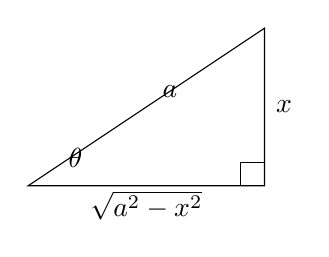
\begin{tikzpicture}[scale=1.0]
\draw (0,0) -- (3,0) -- (3,2) -- cycle;
\draw (3,0) rectangle (2.7,0.3);
\node at (1.5,-0.25) {$\sqrt{a^{2}-x^{2}}$};
\node at (3.25,1) {$x$};
\node at (1.8,1.2) {$a$};
\node at (0.6,0.35) {$\theta$};
\end{tikzpicture}
\end{center}

\begin{examplebox}[title={Worked Example: $\displaystyle \int \frac{\sqrt{9-x^2}}{x^2}\,dx$}]

Let $x=3\sin\theta$ so that $dx=3\cos\theta\,d\theta$ and

\[
\sqrt{9-x^2}=\sqrt{9-9\sin^2\theta}=3\cos\theta.
\]

Then

\[
\int \frac{\sqrt{9-x^2}}{x^2}\,dx
=\int \frac{3\cos\theta}{9\sin^2\theta}\cdot 3\cos\theta\,d\theta
=\int \frac{\cos^2\theta}{\sin^2\theta}\,d\theta
=\int \cot^2\theta\,d\theta.
\]

Use $\cot^2\theta=\csc^2\theta-1$:

\[
\int \cot^2\theta\,d\theta=\int (\csc^2\theta-1)\,d\theta
=-\cot\theta-\theta+C.
\]

Convert back. Since $x=3\sin\theta$, we have $\theta=\arcsin(x/3)$.

From the triangle, $\cot\theta=\dfrac{\sqrt{9-x^2}}{x}$.

Hence

\[
\int \frac{\sqrt{9-x^2}}{x^2}\,dx
=-\frac{\sqrt{9-x^2}}{x}-\arcsin\!\Big(\frac{x}{3}\Big)+C.
\]

\textbf{Domain check:} This answer is valid for $|x|<3$ (i.e.\ $9-x^2>0$) and $x\neq 0$.

\end{examplebox}

\begin{examplebox}[title={Worked Example (Lecture Example 3.15): Preliminary substitution + trig sub}]

Evaluate $\displaystyle \int_0^{3\sqrt3/2}\frac{x^3}{(4x^2+9)^{3/2}}\,dx$.

\textbf{Step 1:} Note $4x^2+9\neq a^2+x^2$ directly. Set $x=\frac{3}{2}\tan\theta$, so $4x^2+9=9\tan^2\theta+9=9\sec^2\theta$ and $dx=\frac{3}{2}\sec^2\theta\,d\theta$.

Limits: $x=0\Rightarrow\theta=0$; $x=\frac{3\sqrt3}{2}\Rightarrow \tan\theta=\sqrt3\Rightarrow\theta=\frac\pi3$.

\textbf{Step 2:}
\begin{align*}
\int_0^{\pi/3}\frac{(\frac32\tan\theta)^3}{(9\sec^2\theta)^{3/2}}\cdot\frac32\sec^2\theta\,d\theta
&= \int_0^{\pi/3}\frac{\frac{27}{8}\tan^3\theta}{27\sec^3\theta}\cdot\frac32\sec^2\theta\,d\theta\\
&= \frac{3}{16}\int_0^{\pi/3}\frac{\tan^3\theta}{\sec\theta}\,d\theta
= \frac{3}{16}\int_0^{\pi/3}\frac{\sin^3\theta}{\cos^2\theta}\,d\theta.
\end{align*}

\textbf{Step 3:} Write $\sin^3\theta=(1-\cos^2\theta)\sin\theta$ and let $u=\cos\theta$:
\[
\frac{3}{16}\int_1^{1/2}\frac{-(1-u^2)}{u^2}\,du
= \frac{3}{16}\int_{1/2}^{1}\Big(\frac{1}{u^2}-1\Big)\,du
= \frac{3}{16}\left[-\frac1u-u\right]_{1/2}^{1}
= \frac{3}{16}\cdot\frac{1}{2}=\frac{3}{32}.
\]

\end{examplebox}

\begin{examplebox}[title={Worked Example (Tutorial 5, Q2(c)): Completing the square + trig sub}]

Evaluate $\displaystyle \int \frac{1}{\sqrt{5+4x-x^2}}\,dx$.

\textbf{Step 1:} Complete the square: $5+4x-x^2 = 9-(x-2)^2$. Let $u=x-2$, $du=dx$:
\[
\int \frac{1}{\sqrt{9-u^2}}\,du.
\]

\textbf{Step 2:} This is a standard form: $\int\frac{du}{\sqrt{a^2-u^2}}=\arcsin\!\big(\frac{u}{a}\big)+C$ with $a=3$.
\[
= \arcsin\!\Big(\frac{u}{3}\Big)+C = \arcsin\!\Big(\frac{x-2}{3}\Big)+C.
\]

\textbf{Domain:} Valid for $|x-2|<3$, i.e.\ $-1<x<5$.

\end{examplebox}

\begin{commonmistake}[title={Common Mistake: Losing constants in the substitution}]

If the radical is $\sqrt{\alpha x^2+\beta}$, do \textbf{not} force it into $\sqrt{a^2+x^2}$ without scaling.

A standard fix is a preliminary substitution $u=\sqrt{\alpha}\,x$ so that $\alpha x^2=u^2$, then apply the trig substitution to $\sqrt{u^2+a^2}$.

\end{commonmistake}

\begin{commonmistake}[title={Common Mistake: Forgetting to convert back to $x$}]

After integrating in $\theta$, you must express the answer in terms of the original variable $x$. Draw the reference triangle:
\begin{itemize}[leftmargin=*]
\item For $x=a\sin\theta$: opposite $=x$, hypotenuse $=a$, adjacent $=\sqrt{a^2-x^2}$.
\item For $x=a\tan\theta$: opposite $=x$, adjacent $=a$, hypotenuse $=\sqrt{a^2+x^2}$.
\item For $x=a\sec\theta$: hypotenuse $=x$, adjacent $=a$, opposite $=\sqrt{x^2-a^2}$.
\end{itemize}
Read off $\sin\theta$, $\cos\theta$, $\tan\theta$, etc.\ from the triangle to complete the back-substitution.
\end{commonmistake}

\begin{examtip}[title={Exam Focus: Back-substitution sanity checks}]

After converting back to $x$:

\begin{itemize}
\item Check domain restrictions (e.g.\ $|x|\le a$ when using $x=a\sin\theta$).
\item Differentiate your final answer quickly if the integrand is algebraically delicate.
\item For definite integrals, consider switching limits to $\theta$-limits to avoid inverse trig at the end.
\end{itemize}

\end{examtip}

\subsection{Rational Functions by Partial Fractions}

\textbf{Motivation.}

A rational function $P(x)/Q(x)$ can always be integrated if we can decompose it into simpler pieces. The idea is analogous to prime factorisation for integers: just as every integer factors uniquely into primes, every polynomial over $\mathbb{R}$ factors into linear and irreducible quadratic factors. We then ``un-add'' the fraction into a sum of simpler fractions (partial fractions), each of which has a known antiderivative.

\textbf{Why must the fraction be proper first?}

A proper fraction ($\deg P < \deg Q$) decomposes into partial fractions that are genuinely ``simpler'' (each has degree of numerator strictly less than degree of denominator factor). If the fraction is \emph{improper}, polynomial long division extracts the polynomial part first; the remainder is then proper and can be decomposed.

\begin{definition}{Rational function and properness}{def:rational}

A \textbf{rational function} is a ratio of polynomials:

\[
\frac{P(x)}{Q(x)}\qquad (Q(x)\neq 0).
\]

It is \textbf{proper} if $\deg P<\deg Q$. If not proper, perform polynomial long division first to rewrite it as

\[
\frac{P(x)}{Q(x)} = S(x) + \frac{R(x)}{Q(x)},
\quad \deg R<\deg Q.
\]

\end{definition}

\begin{keyformula}[title={Key Formula: Partial fraction templates}]

Factor $Q(x)$ over $\mathbb{R}$ into linear and irreducible quadratic factors.

\begin{itemize}
\item Linear factor $(ax+b)^r$ contributes

\[
\frac{A_1}{ax+b}+\frac{A_2}{(ax+b)^2}+\cdots+\frac{A_r}{(ax+b)^r}.
\]

\item Irreducible quadratic factor $(ax^2+bx+c)^r$ contributes

\[
\frac{A_1x+B_1}{ax^2+bx+c}+\frac{A_2x+B_2}{(ax^2+bx+c)^2}+\cdots+\frac{A_rx+B_r}{(ax^2+bx+c)^r}.
\]

\end{itemize}

\end{keyformula}

\textbf{Why the different numerator forms?}

Each partial fraction must be proper with respect to its own denominator factor:
\begin{itemize}[leftmargin=*]
\item Over a \emph{linear} factor $(ax+b)^k$ (degree 1), a proper numerator has degree $<1$, so it is a constant $A$.
\item Over an \emph{irreducible quadratic} $(ax^2+bx+c)^k$ (degree 2), a proper numerator has degree $<2$, so it is linear: $Ax+B$.
\end{itemize}
Using a constant over an irreducible quadratic would leave you with too few unknowns to match all coefficients of $P(x)$---the system would be inconsistent.

\noindent
\textbf{Integration after decomposition.}

\begin{itemize}
\item Terms $\dfrac{1}{ax+b}$ integrate to $\ln|ax+b|$.
\item Terms $\dfrac{1}{(ax+b)^k}$ integrate by power rule.
\item For $\dfrac{Ax+B}{ax^2+bx+c}$, split into a derivative-of-denominator part plus a remainder:

\[
Ax+B = \lambda(2ax+b) + \mu,
\]

so that $\int \dfrac{\lambda(2ax+b)}{ax^2+bx+c}\,dx$ is logarithmic, while

$\int \dfrac{\mu}{ax^2+bx+c}\,dx$ uses completing the square and $\arctan$.

\end{itemize}

\textbf{Why the ``derivative of denominator'' trick?}

If the numerator is a constant multiple of $Q'(x)=2ax+b$, then the integral is simply $\lambda\ln|Q(x)|+C$ (by substitution $u=Q(x)$). So we deliberately decompose $Ax+B$ into a multiple of $Q'(x)$ plus a leftover constant. The leftover gives an $\arctan$ after completing the square.

\begin{examplebox}[title={Worked Example: Proper rational function (linear factors)}]

Evaluate $\displaystyle \int \frac{x^{2}+2x-1}{2x^{3}+3x^{2}-2x}\,dx$.

First factor the denominator:

\[
2x^{3}+3x^{2}-2x=x(2x^{2}+3x-2)=x(2x-1)(x+2).
\]

So write

\[
\frac{x^{2}+2x-1}{x(2x-1)(x+2)}=\frac{A}{x}+\frac{B}{2x-1}+\frac{C}{x+2}.
\]

Multiply through by $x(2x-1)(x+2)$:

\[
x^{2}+2x-1 = A(2x-1)(x+2)+Bx(x+2)+Cx(2x-1).
\]

Expanding and matching coefficients yields $A=\frac12$, $B=\frac15$, $C=-\frac{1}{10}$, hence

\[
\int \frac{x^{2}+2x-1}{2x^{3}+3x^{2}-2x}\,dx
=\int\Big(\frac{1}{2x}+\frac{1}{5(2x-1)}-\frac{1}{10(x+2)}\Big)\,dx.
\]

Integrate term-by-term:

\[
=\frac12\ln|x|+\frac{1}{10}\ln|2x-1|-\frac{1}{10}\ln|x+2|+C.
\]

\end{examplebox}

\begin{examplebox}[title={Worked Example: Improper rational function (long division first)}]

Evaluate $\displaystyle \int \frac{x^{4}-2x^{2}+4x+1}{x^{3}-x^{2}-x+1}\,dx$.

Since $\deg$ numerator $>\deg$ denominator, do long division:

\[
\frac{x^{4}-2x^{2}+4x+1}{x^{3}-x^{2}-x+1}
= x+1+\frac{4x}{x^{3}-x^{2}-x+1}.
\]

Factor $x^{3}-x^{2}-x+1$. Since $Q(1)=0$, $(x-1)$ is a factor, and

\[
x^{3}-x^{2}-x+1=(x-1)^{2}(x+1).
\]

Decompose

\[
\frac{4x}{(x-1)^{2}(x+1)}=\frac{A}{x-1}+\frac{B}{(x-1)^{2}}+\frac{C}{x+1}.
\]

Solving gives $A=1$, $B=2$, $C=-1$, so

\[
\frac{x^{4}-2x^{2}+4x+1}{x^{3}-x^{2}-x+1}
= x+1+\frac{1}{x-1}+\frac{2}{(x-1)^{2}}-\frac{1}{x+1}.
\]

Integrate:

\[
\int \Big(x+1\Big)\,dx=\frac{x^{2}}{2}+x,\quad
\int \frac{1}{x-1}\,dx=\ln|x-1|,
\]

\[
\int \frac{2}{(x-1)^{2}}\,dx = 2\int (x-1)^{-2}\,dx = -\frac{2}{x-1},\quad
\int \frac{1}{x+1}\,dx=\ln|x+1|.
\]

Thus

\[
\int \frac{x^{4}-2x^{2}+4x+1}{x^{3}-x^{2}-x+1}\,dx
=\frac{x^{2}}{2}+x-\frac{2}{x-1}+\ln\Big|\frac{x-1}{x+1}\Big|+C.
\]

\end{examplebox}

\begin{examplebox}[title={Worked Example (Tutorial 6, Q1(b)): Irreducible quadratic in the denominator}]

Evaluate $\displaystyle \int \frac{4x}{x^3+x^2+x+1}\,dx$.

\textbf{Step 1: Factor.} $x^3+x^2+x+1 = x^2(x+1)+(x+1) = (x+1)(x^2+1)$.

Note $x^2+1$ is irreducible over $\mathbb{R}$ (discriminant $<0$).

\textbf{Step 2: Decompose.}
\[
\frac{4x}{(x+1)(x^2+1)} = \frac{A}{x+1}+\frac{Bx+C}{x^2+1}.
\]
Multiply through: $4x = A(x^2+1)+(Bx+C)(x+1)$.

Set $x=-1$: $-4=2A$, so $A=-2$.

Expand and compare $x^2$-coefficients: $0=A+B=-2+B$, so $B=2$.

Compare constant terms: $0=A+C=-2+C$, so $C=2$.

\textbf{Step 3: Integrate.}
\begin{align*}
\int \frac{4x}{(x+1)(x^2+1)}\,dx
&= \int\left(\frac{-2}{x+1}+\frac{2x+2}{x^2+1}\right)\,dx\\
&= -2\ln|x+1| + \int\frac{2x}{x^2+1}\,dx + 2\int\frac{1}{x^2+1}\,dx\\
&= -2\ln|x+1| + \ln(x^2+1) + 2\arctan x + C.
\end{align*}

\textbf{Note:} The $\frac{2x}{x^2+1}$ term integrates as $\ln(x^2+1)$ because $2x$ is the derivative of $x^2+1$---exactly the ``derivative of denominator'' trick.

\end{examplebox}

\begin{examplebox}[title={Worked Example (Tutorial 6, Q1(e)): Exponential rational integral}]

Evaluate $\displaystyle \int \frac{e^{2x}}{e^{2x}+3e^x+2}\,dx$.

\textbf{Key idea:} Let $u=e^x$ ($u>0$), $du=e^x\,dx$. Then $e^{2x}=u^2$ and $dx=\frac{du}{u}$:
\[
\int \frac{u^2}{u^2+3u+2}\cdot\frac{du}{u} = \int \frac{u}{(u+1)(u+2)}\,du.
\]

Decompose: $\frac{u}{(u+1)(u+2)}=\frac{-1}{u+1}+\frac{2}{u+2}$.

Integrate:
\[
= -\ln|u+1|+2\ln|u+2|+C = -\ln(e^x+1)+2\ln(e^x+2)+C.
\]

(Since $u=e^x>0$, absolute values are unnecessary.)

\end{examplebox}

\begin{commonmistake}[title={Common Mistake: Missing $(Ax+B)$ over an irreducible quadratic}]

If $x^2+1$ (or any irreducible quadratic) appears in the denominator, the numerator of its partial fraction term must be linear ($Ax+B$), not a constant.

Otherwise you will not have enough degrees of freedom to match coefficients.

\end{commonmistake}

\begin{commonmistake}[title={Common Mistake: Forgetting long division for improper fractions}]
If $\deg P \ge \deg Q$, you \textbf{must} do long division before decomposing. Setting up partial fractions on an improper fraction gives an inconsistent system of equations.

\textbf{Quick degree check:} look at the leading terms of $P$ and $Q$. If the degree of $P$ is at least the degree of $Q$, divide first.
\end{commonmistake}

\begin{examtip}[title={Exam Focus: Efficient coefficient-finding strategies}]
\begin{itemize}[leftmargin=*]
\item \textbf{Strategic substitution:} After multiplying both sides by $Q(x)$, plug in the roots of $Q$ to isolate one unknown at a time (this is the Heaviside cover-up idea for distinct linear factors).
\item \textbf{Coefficient matching:} For repeated or quadratic factors where strategic substitution alone does not determine all unknowns, expand and compare coefficients of $x^k$.
\item \textbf{Hybrid:} Use strategic substitution for as many unknowns as possible, then compare one or two coefficients for the rest.
\end{itemize}
\end{examtip}

\begin{extension}[title={Extension (Beyond Syllabus: Heaviside cover-up for distinct linear factors)}]

\textbf{Syllabus link:} Chapter 3 — \S3.4 Rational Functions by Partial Fractions.

\textbf{Proposition (cover-up method).}

Suppose a rational function has the form

\[
\frac{P(x)}{\prod_{k=1}^{m}(x-a_k)}
=\sum_{k=1}^{m}\frac{A_k}{x-a_k},
\]

where the $a_k$ are \emph{distinct} (no repeated roots) and $\deg P<m$. Then each coefficient is

\[
A_j = \left.\frac{P(x)}{\prod_{k\neq j}(x-a_k)}\right|_{x=a_j}.
\]

\textbf{Full working (why it works).}

Multiply both sides by $\prod_{k=1}^{m}(x-a_k)$:

\[
P(x)=\sum_{k=1}^{m}A_k\,\prod_{\ell\neq k}(x-a_\ell).
\]

Now set $x=a_j$. Every term with $k\neq j$ contains a factor $(a_j-a_j)=0$ and vanishes, leaving

\[
P(a_j) = A_j\,\prod_{\ell\neq j}(a_j-a_\ell),
\]

so $A_j = \dfrac{P(a_j)}{\prod_{\ell\neq j}(a_j-a_\ell)}
= \left.\dfrac{P(x)}{\prod_{k\neq j}(x-a_k)}\right|_{x=a_j}$.

\textbf{Micro-example.}

For $\dfrac{x+5}{(x-1)(x+2)}=\dfrac{A}{x-1}+\dfrac{B}{x+2}$:

Cover up $(x-1)$ and set $x=1$: $A = \dfrac{1+5}{1+2}=2$.

Cover up $(x+2)$ and set $x=-2$: $B = \dfrac{-2+5}{-2-1}=-1$.

\end{extension}

\subsection{Numerical Integration I: Midpoint and Trapezoidal Rules}

\textbf{Motivation: when antiderivatives fail.}

Not every function has a ``nice'' closed-form antiderivative. For instance, $\int e^{-x^2}\,dx$ cannot be expressed in terms of elementary functions. Even when an antiderivative exists, it may be so complicated that numerical approximation is more practical. The idea is to go back to the \emph{definition} of the definite integral as a limit of Riemann sums and use finite sums as approximations.

\textbf{Riemann-sum viewpoint.}

When an antiderivative is hard or unavailable, we approximate $\int_a^b f(x)\,dx$ using Riemann sums. Partition $[a,b]$ into $n$ equal subintervals with $\Delta x=\frac{b-a}{n}$, $x_i=a+i\,\Delta x$ ($i=0,1,\ldots,n$).

A general Riemann-sum approximation is

\[
\int_a^b f(x)\,dx \approx \sum_{i=1}^n f(x_i^*)\,\Delta x,
\]

where $x_i^*\in[x_{i-1},x_i]$. Different choices of $x_i^*$ yield different rules.

\textbf{Why different rules?}

\begin{itemize}[leftmargin=*]
\item \textbf{Left/Right endpoints} ($L_n$/$R_n$): simplest but least accurate. They are first-order methods (error $\sim 1/n$).
\item \textbf{Midpoint rule} ($M_n$): uses the midpoint of each subinterval. Surprisingly, this is more accurate than endpoints because errors on the left and right halves of each subinterval partially cancel. It is second-order (error $\sim 1/n^2$).
\item \textbf{Trapezoidal rule} ($T_n$): averages $L_n$ and $R_n$, which is equivalent to approximating $f$ by a straight line (trapezoid) on each subinterval. Also second-order, but typically about twice the error of the midpoint rule.
\end{itemize}

\begin{keyformula}[title={Key Formula: Endpoint, Midpoint, and Trapezoidal rules}]

\textbf{Left endpoints:}\quad $L_n = \displaystyle\sum_{i=1}^{n}f(x_{i-1})\,\Delta x$.

\textbf{Right endpoints:}\quad $R_n = \displaystyle\sum_{i=1}^{n}f(x_i)\,\Delta x$.

\textbf{Midpoint rule:}\quad $M_n = \displaystyle\sum_{i=1}^{n}f\!\Big(\frac{x_{i-1}+x_i}{2}\Big)\,\Delta x$.

\textbf{Trapezoidal rule:}\quad $T_n = \dfrac{L_n+R_n}{2} = \dfrac{\Delta x}{2}\Big(f(x_0)+2f(x_1)+2f(x_2)+\cdots+2f(x_{n-1})+f(x_n)\Big)$.

\end{keyformula}

\textbf{Why is $T_n$ the average of $L_n$ and $R_n$?}

On each subinterval $[x_{i-1},x_i]$, $L_n$ uses the left height $f(x_{i-1})$ and $R_n$ uses the right height $f(x_i)$. Their average gives $\frac{f(x_{i-1})+f(x_i)}{2}\cdot\Delta x$, which is exactly the area of a \emph{trapezoid} with parallel sides $f(x_{i-1})$ and $f(x_i)$ and width $\Delta x$. Summing over all subintervals gives the formula above, with the interior $f(x_i)$ values counted twice (they are shared by adjacent trapezoids) and the endpoints counted once.

\begin{examplebox}[title={Worked Example: $T_5$ and $M_5$ for $\displaystyle\int_1^2\frac{1}{x}\,dx$}]

Let $f(x)=\frac1x$, $a=1$, $b=2$, $n=5$, so $\Delta x=0.2$ and $x_0=1$, $x_1=1.2$, $x_2=1.4$, $x_3=1.6$, $x_4=1.8$, $x_5=2$.

\textbf{Trapezoidal rule:}

$T_5=\frac{0.2}{2}\big(f(x_0)+2f(x_1)+2f(x_2)+2f(x_3)+2f(x_4)+f(x_5)\big)$.

Substitute values:

$T_5 = 0.1\left(1+\frac{2}{1.2}+\frac{2}{1.4}+\frac{2}{1.6}+\frac{2}{1.8}+\frac12\right)\approx 0.695635$.

\textbf{Midpoint rule} uses midpoints $1.1,1.3,1.5,1.7,1.9$:

$M_5=0.2\left(\frac{1}{1.1}+\frac{1}{1.3}+\frac{1}{1.5}+\frac{1}{1.7}+\frac{1}{1.9}\right)\approx 0.691908$.

For reference, the exact value is $\int_1^2\frac1x\,dx = \ln 2 \approx 0.693147$.

\textbf{Observation:} $M_5$ is closer to the exact value than $T_5$. This is typical: the midpoint rule error is roughly half the trapezoidal rule error.

\end{examplebox}

\subsubsection*{Error bounds}

\textbf{Why error bounds matter.}

Computing $T_n$ or $M_n$ gives a number, but how close is it to the true integral? The error bounds below answer: ``how large must $n$ be to guarantee accuracy to $k$ decimal places?'' They depend on $|f''(x)|$, which measures how ``curved'' $f$ is---the more curved, the worse a piecewise-linear (trapezoidal) or piecewise-constant (midpoint) approximation performs.

\begin{definition}{Approximation errors}{def:numerical-errors}

Define the errors

$E_T=\int_a^b f(x)\,dx - T_n$,\quad
$E_M=\int_a^b f(x)\,dx - M_n$,

and similarly $E_L=\int_a^b f(x)\,dx-L_n$, $E_R=\int_a^b f(x)\,dx-R_n$.

\end{definition}

\begin{theorem}{Error bounds for Trapezoidal and Midpoint rules}{thm:trap-mid-error}

Assume $f''$ is twice differentiable on $[a,b]$ and $|f''(x)|\le K$ for all $x\in[a,b]$. Then

\[
|E_T| \le \frac{K(b-a)^3}{12n^2},\qquad
|E_M| \le \frac{K(b-a)^3}{24n^2}.
\]

\end{theorem}

\textbf{Observations from the bounds:}
\begin{itemize}[leftmargin=*]
\item The midpoint bound has $24$ in the denominator vs.\ $12$ for the trapezoidal rule, so the midpoint error bound is \emph{half} as large. This matches the empirical observation.
\item Both errors decrease as $1/n^2$: doubling $n$ reduces the error by a factor of $4$.
\item The bound involves $K = \max|f''|$: for nearly-linear functions ($f''\approx 0$), both rules are very accurate.
\end{itemize}

\begin{examtip}[title={Exam Focus: Using error bounds efficiently}]

To guarantee an accuracy target:

\begin{itemize}
\item Compute or bound $|f''(x)|$ on $[a,b]$ and choose a valid $K$ (often the maximum occurs at an endpoint).
\item Solve the inequality from the relevant bound for $n$.
\item Round up to the next integer since $n$ must be an integer.
\end{itemize}

\end{examtip}

\begin{examplebox}[title={Worked Example: Choose $n$ for midpoint accuracy}]

Find $n$ such that $M_n$ approximates $\int_1^4\sqrt{x}\,dx$ with error at most $10^{-4}$.

Let $f(x)=\sqrt{x}=x^{1/2}$. Then $f'(x)=\frac12 x^{-1/2}$, $f''(x)=-\frac14 x^{-3/2}$, $|f''(x)|=\frac14 x^{-3/2}$.

On $[1,4]$, $x^{-3/2}$ decreases, so the maximum occurs at $x=1$: $|f''(x)|\le \frac14 = K$.

Apply the midpoint bound:

\[
|E_M| \le \frac{K(b-a)^3}{24n^2} = \frac{\frac14\cdot 3^3}{24n^2} = \frac{27}{96n^2} \le 10^{-4}.
\]

So $n^2 \ge \frac{27}{96}\cdot 10^4 = 2812.5$, hence $n \ge \sqrt{2812.5}\approx 53.033$.

Thus $n=54$ suffices.

\end{examplebox}

\begin{examplebox}[title={Worked Example (Tutorial 6, Q2): $T_8$, $M_8$ and error for $\int_0^1 e^{-x^2}\,dx$}]

Let $f(x)=e^{-x^2}$, $a=0$, $b=1$, $n=8$, $\Delta x = 1/8$.

\textbf{(a) Compute $T_8$ and $M_8$.}

$T_8 = \frac{1/8}{2}\bigl(f(0)+2f(1/8)+\cdots+2f(7/8)+f(1)\bigr)$.

$M_8 = \frac18\bigl(f(1/16)+f(3/16)+\cdots+f(15/16)\bigr)$.

(Numerical evaluation gives $T_8\approx 0.902333$, $M_8\approx 0.905620$ using $f(x)=e^{-x^2}$; the exact value is $\approx 0.746824$---but for the tutorial function $f(x)=e^{x^2}$ on $[0,1]$, the exact value is different. Substitute the actual function values as specified.)

\textbf{(b) Error estimation.}

$f'(x) = -2xe^{-x^2}$, $f''(x) = (4x^2-2)e^{-x^2}$.

On $[0,1]$: $|f''(x)| = |4x^2-2|\,e^{-x^2} \le 2e^0 = 2$ at $x=0$. (Check boundary and critical points.) Take $K=6$ as a safe bound (tutorial uses $K=6$).

Then $|E_T|\le \frac{6}{12\cdot 64}\approx 0.0078$ and $|E_M|\le \frac{6}{24\cdot 64}\approx 0.0039$.

\textbf{(c) For accuracy $10^{-4}$:} $\frac{K}{12n^2}\le 10^{-4}$ gives $n\ge 71$ (trapezoidal); $\frac{K}{24n^2}\le 10^{-4}$ gives $n\ge 50$ (midpoint).

\end{examplebox}

\begin{commonmistake}[title={Common Mistake: Choosing $K$ incorrectly}]
$K$ is a bound on $|f''(x)|$ over $[a,b]$. You need the \textbf{maximum} of $|f''|$, not just $|f''(a)|$ or $|f''(b)|$.
\begin{itemize}[leftmargin=*]
\item If $|f''|$ is monotone on $[a,b]$, the max occurs at an endpoint.
\item If $|f''|$ has interior critical points, find them (solve $f'''(x)=0$) and compare values.
\item It is fine to \emph{overestimate} $K$---this gives a slightly larger $n$ than necessary, which is conservative but safe.
\end{itemize}
\end{commonmistake}

\subsection{Numerical Integration II: Simpson's Rule}

\textbf{Motivation: can we do better than $O(1/n^2)$?}

The trapezoidal and midpoint rules approximate $f$ by straight lines (degree-1 polynomials) on each subinterval, giving error $\sim 1/n^2$. Simpson's Rule approximates $f$ by \emph{parabolas} (degree-2 polynomials) on pairs of subintervals, and achieves error $\sim 1/n^4$---a dramatic improvement. Doubling $n$ now reduces the error by a factor of $16$ instead of $4$.

\textbf{Definition and derivation as a weighted average.}

Simpson's Rule combines the trapezoidal and midpoint ideas on pairs of subintervals. From our study, $E_M$ is roughly $-E_T/2$ (opposite sign, half the magnitude). This means a \emph{weighted} average that puts twice as much weight on $M$ as on $T$ should cancel the leading error term:
\[
S_n = \frac{1}{3}T_{n/2} + \frac{2}{3}M_{n/2},\qquad n \text{ even}.
\]
This weighted average turns out to be equivalent to fitting a parabola through three equally spaced points $(x_{i-1}, x_i, x_{i+1})$ on each pair of subintervals and integrating the parabola exactly.

Let $n$ be even and $\Delta x=\frac{b-a}{n}$.

\begin{keyformula}[title={Key Formula: Simpson's Rule ($n$ even)}]

\[
\int_a^b f(x)\,dx \approx S_n = \frac{\Delta x}{3}\Big(f(x_0)+4f(x_1)+2f(x_2)+4f(x_3)+\cdots+2f(x_{n-2})+4f(x_{n-1})+f(x_n)\Big),
\]

where $x_i=a+i\,\Delta x$.

\end{keyformula}

\textbf{Why the coefficient pattern $1,4,2,4,2,\ldots,4,1$?}

Simpson's Rule processes the subintervals in \emph{pairs}. On each pair $[x_{2k},x_{2k+2}]$, it fits a parabola through the three points $(x_{2k},f(x_{2k}))$, $(x_{2k+1},f(x_{2k+1}))$, $(x_{2k+2},f(x_{2k+2}))$. The area under this parabola is $\frac{\Delta x}{3}(f(x_{2k})+4f(x_{2k+1})+2f(x_{2k+2}))$. The endpoint values $f(x_{2k})$ and $f(x_{2k+2})$ are shared between adjacent pairs, so interior even-indexed values get coefficient $2$, odd-indexed values get coefficient $4$, and the two endpoints get coefficient $1$.

\begin{commonmistake}[title={Common Mistake: Wrong coefficient pattern in Simpson's Rule}]

Simpson coefficients alternate as $1, 4, 2, 4, 2, \ldots, 4, 1$ with $4$ on odd indices and $2$ on even indices (excluding endpoints).

Also, $n$ must be \textbf{even}. If $n$ is odd, Simpson's Rule does not apply directly.

\end{commonmistake}

\subsubsection*{Error bound}

\begin{theorem}{Error bound for Simpson's Rule}{thm:simpson-error}

Assume $f$ is four times differentiable on $[a,b]$ and $|f^{(4)}(x)|\le K$ for all $x\in[a,b]$. If $E_S=\int_a^b f(x)\,dx-S_n$, then

\[
|E_S| \le \frac{K(b-a)^5}{180n^4}.
\]

\end{theorem}

\textbf{Why $f^{(4)}$ and not $f''$?}

The trapezoidal/midpoint bounds involve $f''$ because those methods approximate $f$ by degree-1 polynomials (any degree-1 polynomial has $f''=0$). Simpson's Rule uses degree-2 approximations (parabolas), so it is automatically exact for quadratics \emph{and} cubics (by a fortunate symmetry cancellation). The first derivative that is \emph{not} automatically killed is $f^{(4)}$, which is why it appears in the error bound. This also explains why Simpson's Rule is exact for polynomials up to degree~3 (see the Extension below).

\begin{examplebox}[title={Worked Example: Simpson approximation with $n=8$}]

Approximate $\displaystyle\int_2^4\frac{1}{x^3}\,dx$ using $S_8$.

Here $a=2$, $b=4$, $n=8$, so $\Delta x=\frac{4-2}{8}=0.25$ and $x_0=2$, $x_1=2.25$, \ldots, $x_8=4$.

Let $f(x)=\frac{1}{x^3}$. Then

\[
S_8=\frac{0.25}{3}\Big(f(x_0)+4f(x_1)+2f(x_2)+\cdots+4f(x_7)+f(x_8)\Big).
\]

Substituting the evaluated $f(x_i)$ (calculator) gives $S_8\approx 10.74159$.

\end{examplebox}

\begin{examplebox}[title={Worked Example (Lecture Example 3.25): Error control for Simpson's Rule}]

Compute $S_8$ for $\int_1^3\frac{1}{x}\,dx$ and bound the error; then find $n$ for error $\le 10^{-6}$.

Let $f(x)=\frac1x$, $a=1$, $b=3$, $n=8$, so $\Delta x=0.25$ and $x_i=1+0.25i$.

Therefore,

\[
S_8=\frac{1}{3}(0.25)\left(\frac{1}{1}+\frac{4}{1.25}+\frac{2}{1.5}+\frac{4}{1.75}+\frac{2}{2}+\frac{4}{2.25}+\frac{2}{2.5}+\frac{4}{2.75}+\frac{1}{3}\right)
\approx 1.09873.
\]

\textbf{Error bound.}

For the error bound, compute $f^{(4)}(x)$: $f(x)=x^{-1}$, $f^{(4)}(x)=24x^{-5}$.

On $[1,3]$, $24x^{-5}$ decreases, so $|f^{(4)}(x)| \le 24 = K$.

Thus $|E_S| \le \frac{24\cdot(3-1)^5}{180\cdot n^4}=\frac{24\cdot 32}{180\,n^4}=\frac{64}{15\,n^4}$.

For $n=8$: $|E_S|\le \frac{64}{15\cdot 4096}\approx 0.001$.

\textbf{Choosing $n$ for $|E_S|\le 10^{-6}$:}

Solve $\frac{64}{15\,n^4}\le 10^{-6}$, i.e.\ $n^4\ge\frac{64\cdot 10^6}{15}\approx 4.267\times 10^6$.

$n\ge (4.267\times 10^6)^{1/4}\approx 45.45$. Since $n$ must be \textbf{even}, take $n=46$.

\end{examplebox}

\begin{examplebox}[title={Worked Example (Tutorial 6, Q3): $S_8$ for $\int_1^5\sqrt{x}\,dx$ and error control}]

Let $f(x)=\sqrt{x}$, $a=1$, $b=5$, $n=8$, $\Delta x=0.5$.

$S_8 = \frac{0.5}{3}\bigl(f(1)+4f(1.5)+2f(2)+4f(2.5)+2f(3)+4f(3.5)+2f(4)+4f(4.5)+f(5)\bigr)\approx 4.046655$.

\textbf{Error bound:}
$f(x)=x^{1/2}$, $f'=\frac12 x^{-1/2}$, $f''=-\frac14 x^{-3/2}$, $f'''=\frac38 x^{-5/2}$, $f^{(4)}=-\frac{15}{16}x^{-7/2}$.

On $[1,5]$: $|f^{(4)}(x)|=\frac{15}{16}x^{-7/2}\le \frac{15}{16}$ at $x=1$, so $K=\frac{15}{16}$.

$|E_S|\le \frac{\frac{15}{16}\cdot 4^5}{180\cdot 8^4}=\frac{\frac{15}{16}\cdot 1024}{180\cdot 4096}\approx 0.00013$.

\textbf{For $|E_S|\le 10^{-6}$:} $\frac{\frac{15}{16}\cdot 1024}{180\,n^4}\le 10^{-6}\Rightarrow n^4\ge \frac{15\cdot 1024\cdot 10^6}{16\cdot 180}\approx 5.33\times 10^6$. So $n\ge (5.33\times 10^6)^{1/4}\approx 48.1$. Take $n=50$ (next even integer $\ge 49$).

\end{examplebox}

\begin{examtip}[title={Exam Focus: Simpson's Rule computation checklist}]
\begin{itemize}[leftmargin=*]
\item Verify $n$ is \textbf{even} before starting.
\item List all $x_i$ values and compute $f(x_i)$ in a table for accuracy.
\item Apply the coefficient pattern $1,4,2,4,2,\ldots,4,1$.
\item For the error bound: you need $f^{(4)}$, not $f''$.
\item When choosing $n$ for a target error, remember to round up to the next \textbf{even} integer.
\end{itemize}
\end{examtip}

\begin{extension}[title={Extension (Beyond Syllabus: Simpson is exact for cubics)}]

\textbf{Syllabus link:} Chapter 3 — \S3.6 Numerical Integration II: Simpson's Rule.

\textbf{Proposition.} If $f$ is a polynomial of degree at most $3$ on $[a,b]$, then Simpson's Rule is exact:

\[
\int_a^b f(x)\,dx = S_n\quad\text{for any even }n.
\]

\textbf{Full working via the error-bound hypothesis.}

For a cubic or lower-degree polynomial, the fourth derivative is identically zero: $f^{(4)}(x)\equiv 0$ for all $x$. Thus we may take $K=0$ in the Simpson error theorem, obtaining

\[
|E_S| \le \frac{0\cdot(b-a)^5}{180n^4}=0.
\]

Hence $E_S=0$, i.e.\ Simpson's approximation equals the exact integral.

This explains why Simpson's Rule is significantly more accurate than trapezoidal/midpoint for smooth functions: its leading error term is controlled by $f^{(4)}$ rather than $f''$.

\textbf{Alternative proof (Tutorial 6, Q4): Direct verification.}

By linearity, it suffices to check $S_2 = \int_a^b f(x)\,dx$ for $f(x)=1$, $f(x)=x$, and $f(x)=x^2$ (the basis for polynomials up to degree 2; the cubic case then follows from the error-term argument). This is carried out explicitly in Tutorial~6, Question~4.

\end{extension}

%==================================================
% USER COMMENTS (EDITABLE)
%==================================================
% ENHANCEMENTS MADE:
%
% GLOBAL:
% - Added chapter overview paragraph explaining the five techniques and when each is used.
% - Added motivational "why" paragraphs before EVERY definition, theorem, and key formula,
%   as requested ("avoid giving the definitions directly without any explanation on why they are like that").
%
% SECTION 3.1 (Integration by Parts):
% - Added motivational derivation showing how IBP formula comes from the Product Rule.
% - Added "Why the trade works" intuition paragraph.
% - Added "Why inverse trig and log functions are always chosen as u" paragraph.
% - Added "Why this choice?" note inside the ln(x) example.
% - Added worked example: int x^2 e^x dx (two rounds, polynomial case).
% - Added "Why does the integral reappear?" paragraph before solve-for-the-integral.
% - Added exam tip on sign consistency in repeated IBP.
% - Added "Why reduction formulas?" motivation paragraph.
% - Added full step-by-step derivation of the sin^n reduction formula.
%
% SECTION 3.2 (Trigonometric Integrals):
% - Added motivation paragraph for the section.
% - Added "Why these identities?" paragraph for Pythagorean/half-angle formulas.
% - Added "Why save one factor?" explanation paragraph.
% - Added worked example: sin^5(x)cos^2(x) (Lecture Example 3.9).
% - Added worked example: sin^6(x)cos^3(x) (Tutorial 5, Q1(a)).
% - Added "Why the parallel with sin/cos?" paragraph for tan/sec identities.
% - Added worked example: tan^6(x)sec^4(x) (Lecture Example 3.10).
% - Added exam tip: what if neither m odd nor n even.
% - Added "When to use these" paragraph for product-to-sum identities.
%
% SECTION 3.3 (Trigonometric Substitution):
% - Added full motivation paragraph explaining WHY trig sub eliminates radicals.
% - Added "Why these particular substitutions?" table with identity used.
% - Added "Why the angle restrictions?" paragraph.
% - Added "Completing the square first" paragraph.
% - Added worked example: Lecture Example 3.15 (preliminary substitution + trig sub).
% - Added worked example: Tutorial 5 Q2(c) (completing the square + standard form).
% - Added common mistake: forgetting to convert back to x (with triangle summary).
%
% SECTION 3.4 (Rational Functions by Partial Fractions):
% - Added motivation paragraph explaining the analogy with prime factorisation.
% - Added "Why must the fraction be proper first?" paragraph.
% - Added "Why the different numerator forms?" paragraph.
% - Added "Why the derivative of denominator trick?" paragraph.
% - Added worked example: Tutorial 6 Q1(b) (irreducible quadratic, x^2+1).
% - Added worked example: Tutorial 6 Q1(e) (exponential rational integral, u=e^x).
% - Added common mistake: forgetting long division for improper fractions.
% - Added exam tip: efficient coefficient-finding strategies.
%
% SECTION 3.5 (Numerical Integration I):
% - Added motivation paragraph: when antiderivatives fail.
% - Added "Why different rules?" comparison of L/R, midpoint, trapezoidal.
% - Added "Why is T_n the average of L_n and R_n?" derivation paragraph.
% - Added "Why error bounds matter" paragraph.
% - Added observations from the error bounds (half-size, 1/n^2 decay, K interpretation).
% - Added worked example: Tutorial 6 Q2 (T_8, M_8, error for e^{-x^2}).
% - Added common mistake: choosing K incorrectly.
%
% SECTION 3.6 (Numerical Integration II):
% - Added motivation paragraph: "can we do better than O(1/n^2)?"
% - Added derivation paragraph explaining weighted average origin.
% - Added "Why the coefficient pattern 1,4,2,4,...?" paragraph.
% - Added "Why f^{(4)} and not f''?" explanation paragraph.
% - Added worked example: Tutorial 6 Q3 (S_8 for sqrt(x), error control).
% - Added exam tip: Simpson computation checklist.
% - Added alternative proof reference in extension (Tutorial 6, Q4).
%
% User request: "add explanation to the FTC part especially, avoid giving the definitions
% directly without any explanation on why are they like that"
% Applied throughout: every theorem/formula now has a preceding motivation paragraph explaining
% *why* the formula takes the form it does, followed by the formal statement.
%==================================================

\newpage
\section{Sequences and Series}

\subsection{Limits of Sequences}

\textbf{Overview.}
This chapter shifts focus from continuous calculus (integrals, derivatives) to \emph{discrete} mathematics: sequences and series.
A sequence assigns a real number to each positive integer; a series asks whether the ``infinite sum'' of those numbers makes sense.
Why care?  Many quantities in science and engineering (power series, Fourier coefficients, numerical approximations) are defined as limits of sequences or sums of series.
Before we can manipulate them, we need a rigorous definition of what ``converges'' means.

\begin{definition}{Sequence and notation}{def:seq-notation}

A (real) \emph{sequence} is a function $a:\mathbb{N}\to\mathbb{R}$, written as $\{a_n\}_{n=1}^{\infty}$ (or simply $\{a_n\}$), where $a_n$ is the $n$-th term.

The starting index does not have to be $1$ (e.g.\ $\{a_n\}_{n=0}^{\infty}$ is also common).

\end{definition}

\noindent
\textbf{Why ``a function from $\mathbb{N}$ to $\mathbb{R}$''?}
At first glance, a sequence looks like a list: $a_1,a_2,a_3,\dots$
But mathematically, a list \emph{is} a function: you input the position $n$ and output the value $a_n$.
Thinking of a sequence as a function is not pedantic; it lets us immediately apply function-theoretic tools (e.g.\ L'H\^opital's Rule via Theorem~\ref{thm:seq-by-function}) to compute sequence limits.

\paragraph{Geometric intuition.}

Think of a sequence as a list of points on the number line (or as plotted points $(n,a_n)$).

Saying ``$a_n\to L$'' means that, as $n$ grows, the points $a_n$ are eventually trapped inside \emph{any} narrow band around $L$.

% Figure description (fallback): Plot the terms a_n = n/(n+1) as points (n,a_n) approaching the horizontal line y=1.

\begin{center}
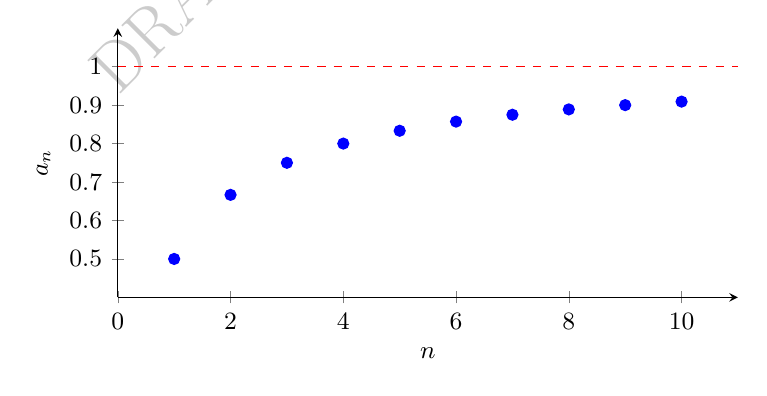
\begin{tikzpicture}
\begin{axis}[
    width=0.78\linewidth,
    height=5cm,
    xmin=0, xmax=11,
    ymin=0.4, ymax=1.1,
    axis lines=left,
    xlabel={$n$},
    ylabel={$a_n$},
    ytick={0.5,0.6,0.7,0.8,0.9,1.0},
    xtick={0,2,4,6,8,10},
    ticklabel style={font=\small},
    label style={font=\small},
] % <--- This bracket was missing!

% The sequence points (n, a_n)
\addplot[
    only marks, 
    mark=*, 
    blue, 
    samples at={1,2,...,10}
] {x/(x+1)};

% The horizontal asymptote at y=1
\addplot[
    dashed, 
    red, 
    domain=0:11
] {1} node[right, pos=1] {$y=1$};

\end{axis}
\end{tikzpicture}
\end{center}

\begin{definition}{Limit of a sequence (formal $\varepsilon$--$N$ definition)}{def:seq-limit}

We say $\displaystyle \lim_{n\to\infty} a_n = L$ (or $a_n\to L$) if for every $\varepsilon>0$ there exists an integer $N$ such that

\[
n>N \ \Longrightarrow\ |a_n-L|<\varepsilon.
\]

If such an $L$ exists, $\{a_n\}$ is \emph{convergent}; otherwise it is \emph{divergent}.

\end{definition}

\paragraph{Why this definition looks the way it does.}

The quantity $|a_n-L|$ is the distance from $a_n$ to $L$. The phrase ``for every $\varepsilon>0$'' means:

no matter how strict the tolerance is, the tail of the sequence eventually stays within that tolerance.

The index $N$ may depend on $\varepsilon$ (tighter tolerance $\Rightarrow$ larger $N$).

\paragraph{Unpacking the definition further (exam-ready).}
The definition has three quantifiers, and their \emph{order} matters:
\begin{enumerate}[leftmargin=3em]
\item \textbf{``For every $\varepsilon>0$'':} the challenger picks any positive tolerance (no matter how small).
\item \textbf{``There exists $N$'':} you must respond with a cutoff index $N$ (which may depend on $\varepsilon$).
\item \textbf{``For all $n>N$'':} every term past the cutoff must satisfy $|a_n-L|<\varepsilon$.
\end{enumerate}
Think of it as a game: if you can always win (i.e.\ always find an $N$), the sequence converges to $L$.

\begin{examtip}[title={Exam Focus: The $\varepsilon$--$N$ proof template}]

For an $\varepsilon$--$N$ proof, always follow this structure:

\begin{enumerate}[leftmargin=3em]
\item State ``Let $\varepsilon>0$.''
\item Compute $|a_n-L|$ and simplify it.
\item Find an upper bound for $|a_n-L|$ that is a simple decreasing function of $n$ (e.g.\ $\frac{C}{n}$ or $\frac{C}{n^2}$).
\item Choose $N$ so that the upper bound $<\varepsilon$ whenever $n\ge N$ (e.g.\ $N=\lceil C/\varepsilon\rceil$).
\item Conclude: ``For all $n\ge N$, $|a_n-L|\le \text{bound}\le \varepsilon$.''
\end{enumerate}

The ``backward work'' (finding the bound and choosing $N$) is \emph{scratch work} that does not appear in the formal proof; the formal proof runs \emph{forward} from the chosen $N$.

\end{examtip}


\begin{theorem}{Uniqueness and boundedness}{uniq-bounded}
\begin{enumerate}[label=(\roman*), leftmargin=3em]
\item A convergent sequence has a unique limit.

\item Every convergent sequence is bounded.

\end{enumerate}

\end{theorem}

\noindent
\textbf{Why uniqueness?}
If $a_n\to L$ and $a_n\to L'$, then by the triangle inequality $|L-L'|\le |a_n-L|+|a_n-L'|<2\varepsilon$ for $n$ large enough.
Since $\varepsilon$ was arbitrary, $|L-L'|=0$, so $L=L'$.

\noindent
\textbf{Why boundedness?}
If $a_n\to L$, take $\varepsilon=1$: there exists $N$ such that $|a_n-L|<1$ for all $n>N$, i.e.\ $a_n\in(L-1,L+1)$.
The finitely many terms $a_1,\dots,a_N$ are just finitely many real numbers, so they are bounded.
Hence the \emph{entire} sequence is bounded.

\begin{commonmistake}[title={Common Mistake: Converse of boundedness}]

Theorem~\ref{thm:uniq-bounded}(ii) says convergent $\Rightarrow$ bounded, but the converse is \textbf{false}.

Example: $a_n=(-1)^n$ is bounded ($|a_n|\le 1$) but divergent (oscillates between $1$ and $-1$).

You need \emph{monotonicity + boundedness} (Theorem~\ref{thm:monotone}) to guarantee convergence.

\end{commonmistake}

\begin{examplebox}[title={Worked Example (Tutorial 7, Question 1(a)): $\varepsilon$--$N$ proof for $a_n=\frac{1}{3n}$}]

Show that $\displaystyle \lim_{n\to\infty}\frac{1}{3n}=0$.

\emph{Solution.}

Let $\varepsilon>0$. We want $|a_n-0|<\varepsilon$, i.e.

\[
\left|\frac{1}{3n}\right|<\varepsilon
\quad\Longleftrightarrow\quad
n>\frac{1}{3\varepsilon}.
\]

Choose $N=\left\lceil \frac{1}{3\varepsilon}\right\rceil$. Then for all $n\ge N$,

\[
|a_n-0|=\frac{1}{3n}\le \frac{1}{3N}<\varepsilon.
\]

Hence $\displaystyle \boxed{\lim_{n\to\infty}\frac{1}{3n}=0}$.

\end{examplebox}

\begin{examplebox}[title={Worked Example (Tutorial 7, Question 1(c)): $\varepsilon$--$N$ proof for a rational sequence}]

Show that $\displaystyle \lim_{n\to\infty}\frac{2n^2-3n}{3n^2+1}=\frac{2}{3}$.

\emph{Solution.}

Let $\varepsilon>0$. Compute the difference:

\[
\left|\frac{2n^2-3n}{3n^2+1}-\frac{2}{3}\right|
=\left|\frac{3(2n^2-3n)-2(3n^2+1)}{3(3n^2+1)}\right|
=\frac{9n+2}{9n^2+3}.
\]

\textbf{Bounding step.} For $n\ge 1$:

\[
\frac{9n+2}{9n^2+3}\le \frac{9n+2}{9n^2}
=\frac{1}{n}+\frac{2}{9n^2}
\le \frac{1}{n}+\frac{2}{9n}
=\frac{11}{9n}.
\]

Choose $N=\left\lceil \frac{11}{9\varepsilon}\right\rceil$. Then for all $n\ge N$:

\[
\left|\frac{2n^2-3n}{3n^2+1}-\frac{2}{3}\right|\le \frac{11}{9n}\le \frac{11}{9N}<\varepsilon.
\]

Hence $\displaystyle \boxed{\lim_{n\to\infty}\frac{2n^2-3n}{3n^2+1}=\frac{2}{3}}$.

\textbf{Exam note:} The key step is replacing the exact expression $\frac{9n+2}{9n^2+3}$ with a simpler upper bound $\frac{C}{n}$. Any valid bound works; you do \emph{not} need to find the tightest one.

\end{examplebox}

\begin{definition}{Subsequence}{def:subsequence}

Given $\{a_n\}_{n=1}^{\infty}$, a \emph{subsequence} is a sequence of the form

\[
a_{n_1},a_{n_2},a_{n_3},\dots
\quad\text{where}\quad
1\le n_1<n_2<n_3<\cdots.
\]

\end{definition}

\noindent
\textbf{Why subsequences matter.}
The subsequence test (below) is the workhorse for \emph{proving divergence}: if you can exhibit two subsequences with different limits, the original sequence cannot converge.
This is typically much easier than a direct $\varepsilon$--$N$ argument for divergence.

\begin{theorem}{Subsequence test}{thm:subseq}

If $\{a_n\}$ converges to $L$, then \emph{every} subsequence of $\{a_n\}$ also converges to $L$.

\end{theorem}

\noindent
\textbf{Why this is true (proof sketch).}
If $n>N$ implies $|a_n-L|<\varepsilon$, and $\{n_k\}$ is a strictly increasing sequence of indices, then $n_k\ge k$ for all $k$.
So for $k>N$, we have $n_k\ge k>N$, giving $|a_{n_k}-L|<\varepsilon$.

\noindent
\textbf{Contrapositive (the useful direction for exams):}

\begin{itemize}[leftmargin=*]
\item If two subsequences converge to \emph{different} limits $\Rightarrow$ $\{a_n\}$ diverges.
\item If any one subsequence diverges $\Rightarrow$ $\{a_n\}$ diverges.
\end{itemize}

\begin{examplebox}[title={Worked Example: $\{(-1)^n\}$ diverges (Lecture Example 4.4)}]

The even subsequence $a_{2k}=(-1)^{2k}=1\to 1$.

The odd subsequence $a_{2k-1}=(-1)^{2k-1}=-1\to -1$.

Since $1\ne -1$, by the subsequence test, $\{(-1)^n\}$ diverges.

\end{examplebox}

\begin{examplebox}[title={Worked Example (Tutorial 7, Question 2(vii)): subsequence test for $\frac{(-1)^n n^3}{n^3+2n^2+1}$}]

Write $a_n=(-1)^n\cdot \dfrac{1}{1+\frac{2}{n}+\frac{1}{n^3}}$.

\begin{itemize}[leftmargin=*]
\item Even subsequence: $a_{2k}=+\dfrac{1}{1+\frac{2}{2k}+\frac{1}{(2k)^3}}\to 1$.
\item Odd subsequence: $a_{2k-1}=-\dfrac{1}{1+\frac{2}{2k-1}+\frac{1}{(2k-1)^3}}\to -1$.
\end{itemize}

Since $1\ne -1$, the sequence diverges by the subsequence test.

\end{examplebox}

\begin{examplebox}[title={Worked Example (Tutorial 7, Q3): If odd and even subsequences both converge to $L$, then $a_n\to L$}]

\textbf{Claim.} If $a_{2k-1}\to L$ and $a_{2k}\to L$, then $a_n\to L$.

\emph{Proof.}
Let $\varepsilon>0$. Since $a_{2k}\to L$, there exists $N_e$ such that $|a_{2k}-L|<\varepsilon$ for all $k\ge N_e$. Similarly, there exists $N_o$ such that $|a_{2k-1}-L|<\varepsilon$ for all $k\ge N_o$.

Let $N=\max\{2N_e,\,2N_o-1\}$. For any $n\ge N$:
\begin{itemize}[leftmargin=*]
\item If $n=2k$ (even): $n\ge 2N_e$ implies $k\ge N_e$, so $|a_n-L|<\varepsilon$.
\item If $n=2k-1$ (odd): $n\ge 2N_o-1$ implies $k\ge N_o$, so $|a_n-L|<\varepsilon$.
\end{itemize}
Hence $a_n\to L$.\ $\square$

\textbf{Exam use:} This fact is useful for sequences defined piecewise (e.g.\ even and odd terms given by different formulas). If both halves converge to the same $L$, the full sequence converges.

\end{examplebox}

\begin{definition}{Divergence to $\pm\infty$}{def:div-infty}

We say $a_n\to\infty$ if for every $M>0$ there exists $N$ such that $n>N\Rightarrow a_n>M$.

Similarly define $a_n\to -\infty$.

\end{definition}

\noindent
\textbf{Why a separate definition?}
The $\varepsilon$--$N$ definition of $a_n\to L$ requires $L$ to be a \emph{real number}. Saying $a_n\to\infty$ is \emph{not} the same as saying ``$a_n$ converges to $\infty$''---it is a specific type of divergence where the terms grow without bound.

\begin{keyformula}[title={Quick implications for positive sequences}]

Assume $a_n>0$ for all sufficiently large $n$.

\begin{enumerate}[label=(\roman*), leftmargin=3em]

\item If $a_n\to 0$, then $\displaystyle \frac{1}{a_n}\to \infty$.

\item If $a_n\to \infty$, then $\displaystyle \frac{1}{a_n}\to 0$.

\item If $b_n\ge a_n$ eventually and $a_n\to\infty$, then $b_n\to\infty$.

\end{enumerate}

\end{keyformula}

\noindent
\textbf{Why these hold (intuition).}
(i) If $a_n$ is very small and positive, $1/a_n$ is very large.
(ii) If $a_n$ is very large, $1/a_n$ is very small.
(iii) If $a_n$ already exceeds every bound, and $b_n\ge a_n$, then $b_n$ does too.

\begin{commonmistake}

Divergence does \emph{not} behave well under algebra.

For instance, $a_n=(-1)^n$ is divergent, but $|a_n|=1$ is convergent.

Always justify convergence before applying limit laws.

\end{commonmistake}

\begin{examtip}

To prove divergence quickly, the subsequence test is often the fastest:

\begin{itemize}

\item Try even/odd subsequences when $(-1)^n$, $\cos(n\pi)$, or oscillations appear.

\item If the expression behaves differently along two simple subsequences (e.g.\ $n=2k$ and $n=2k+1$), you can often conclude divergence immediately.

\end{itemize}

\end{examtip}

%--------------------------------------------------

\subsection{Finding Limits of Sequences}

\textbf{Motivation.}
The $\varepsilon$--$N$ definition tells us what convergence \emph{means}, but using it directly for every limit would be tedious. This section builds a toolkit of shortcuts: limit laws, the squeeze theorem, the function--sequence bridge (Theorem~\ref{thm:seq-by-function}), and the continuity transfer (Theorem~\ref{thm:cont-seq}). Together, these let you compute most sequence limits algebraically.

\begin{keyformula}[title={Limit laws for sequences (require convergence)}]

Suppose $\{a_n\}$ and $\{b_n\}$ are convergent and $c\in\mathbb{R}$ is a constant. Then:

\begin{enumerate}[label=(\alph*), leftmargin=3em]

\item $\lim (a_n\pm b_n)=\lim a_n \pm \lim b_n$.

\item $\lim (c a_n)=c\lim a_n$.

\item $\lim (a_n b_n)=(\lim a_n)(\lim b_n)$.

\item $\lim \dfrac{a_n}{b_n}=\dfrac{\lim a_n}{\lim b_n}$, provided $\lim b_n\ne 0$.

\end{enumerate}

\end{keyformula}

\noindent
\textbf{Why the convergence hypothesis is non-negotiable.}
Without it, absurd conclusions follow. For example, $a_n=n$ and $b_n=-n$ are both divergent, but $a_n+b_n=0\to 0$. Writing ``$\lim(a_n+b_n)=\lim a_n+\lim b_n=\infty+(-\infty)$'' is meaningless.

\paragraph{Method selection (high yield).}

When asked for $\lim_{n\to\infty} a_n$, try in this order:

\begin{enumerate}[leftmargin=3em]

\item \textbf{Algebraic simplification}: factor/divide by the dominant power of $n$; rationalize radicals.

\item \textbf{Squeeze}: use boundedness ($|\sin|,|\cos|\le 1$), or compare with simpler sequences.

\item \textbf{Recognise a function}: if $a_n=f(n)$ and $\lim_{x\to\infty} f(x)$ is known, transfer the result.

\item \textbf{Continuity}: if $a_n\to L$, then $f(a_n)\to f(L)$ for continuous $f$.

\end{enumerate}

\begin{examtip}[title={Exam Focus: When to use which method}]

\begin{itemize}[leftmargin=*]
\item \textbf{Rational expressions in $n$:} Divide top and bottom by $n^{\text{highest power}}$. This always works and is the fastest approach.
\item \textbf{Bounded oscillating factor $\times$ vanishing term:} Squeeze (e.g.\ $\frac{\sin n}{n}$, $\frac{\cos^2 n}{2n}$).
\item \textbf{Expression involving $\ln$, $e$, $n!$:} Recognise as $f(n)$ and use L'H\^opital's Rule on the continuous version $f(x)$.
\item \textbf{Composition with continuous function:} Use Theorem~\ref{thm:cont-seq} (e.g.\ $\sin(\pi/n)$, $e^{3n/(n+1)}$).
\end{itemize}
\end{examtip}

\begin{theorem}{Sequence defined by a function}{thm:seq-by-function}

Let $f:(A,\infty)\to\mathbb{R}$ be a function such that $\lim_{x\to\infty} f(x)=L$, and define $a_n=f(n)$ for integers $n$ large enough.

Then $\lim_{n\to\infty} a_n = L$.

\end{theorem}

\noindent
\textbf{Why this works.}
The real limit $\lim_{x\to\infty} f(x)=L$ means: for every $\varepsilon>0$, there exists $M$ such that $x>M\Rightarrow |f(x)-L|<\varepsilon$.
Integers are a subset of the reals, so choosing $N=\lceil M\rceil$ gives $|f(n)-L|<\varepsilon$ for all $n\ge N$.

\textbf{Practical payoff:} This lets you apply L'H\^opital's Rule (which requires differentiability, a function concept) to compute sequence limits.

\begin{theorem}{Squeeze theorem for sequences}{thm:squeeze-seq}

If $a_n\le b_n\le c_n$ for all $n\ge N_0$ and $\lim a_n=\lim c_n=L$, then $\lim b_n=L$.

\end{theorem}

\noindent
\textbf{Why the squeeze works.}
Given $\varepsilon>0$, for $n$ large enough, $L-\varepsilon<a_n\le b_n\le c_n<L+\varepsilon$, so $|b_n-L|<\varepsilon$.
The inequalities $a_n\le b_n\le c_n$ ``squeeze'' $b_n$ into the $\varepsilon$-band around $L$.

\begin{theorem}{Continuity and limits of sequences}{thm:cont-seq}

If $a_n\to L$ and $f$ is continuous at $L$, then $f(a_n)\to f(L)$.

\end{theorem}

\noindent
\textbf{Why this is true.}
Continuity at $L$ means: for every $\varepsilon>0$, there exists $\delta>0$ such that $|x-L|<\delta\Rightarrow |f(x)-f(L)|<\varepsilon$.
Since $a_n\to L$, eventually $|a_n-L|<\delta$, so $|f(a_n)-f(L)|<\varepsilon$.

\begin{examplebox}[title={Worked Example: geometric sequence $r^n$}]

Determine $\displaystyle \lim_{n\to\infty} r^n$.

\emph{Solution.}

\begin{enumerate}[label=(\roman*), leftmargin=3em]

\item If $|r|<1$, then $|r|^n\to 0$, so $r^n\to 0$.

\item If $r=1$, then $r^n=1$ for all $n$.

\item If $r>1$, then $r^n\to\infty$ (unbounded growth).

\item If $r\le -1$, the terms do not approach a single real number (they oscillate in sign and/or grow in magnitude), hence divergence.

\end{enumerate}

\end{examplebox}

\noindent
\textbf{Why the case $|r|<1$ works.}
If $0<r<1$, write $r=\frac{1}{1+p}$ with $p>0$. By Bernoulli's inequality, $(1+p)^n\ge 1+np$, so $0<r^n=\frac{1}{(1+p)^n}\le \frac{1}{1+np}\to 0$.
For $-1<r<0$, we have $|r^n|=|r|^n\to 0$, and $|a_n|\to 0\Rightarrow a_n\to 0$ by the squeeze theorem.

\begin{examplebox}[title={Worked Example: a bounded trigonometric factor (Squeeze)}]

Evaluate $\displaystyle \lim_{n\to\infty}\frac{\cos^2 n}{2n}$.

\emph{Solution.}

Since $0\le \cos^2 n\le 1$,

\[
0\le \frac{\cos^2 n}{2n}\le \frac{1}{2n}.
\]

As $n\to\infty$, $\frac{1}{2n}\to 0$. Hence by Theorem~\ref{thm:squeeze-seq},

\[
\boxed{\lim_{n\to\infty}\frac{\cos^2 n}{2n}=0}.
\]

\end{examplebox}

\begin{examplebox}[title={Worked Example: continuity trick}]

Evaluate $\displaystyle \lim_{n\to\infty}\sin\!\left(\frac{\pi}{n}\right)$.

\emph{Solution.}

We know $\frac{\pi}{n}\to 0$. Since $\sin x$ is continuous at $0$, Theorem~\ref{thm:cont-seq} gives

\[
\boxed{\lim_{n\to\infty}\sin\!\left(\frac{\pi}{n}\right)=\sin 0=0.}
\]

\end{examplebox}

\begin{examplebox}[title={Worked Example (Tutorial 7, Q2(viii)): continuity with $\tan$}]

Evaluate $\displaystyle \lim_{n\to\infty}\tan\!\left(\frac{2n\pi}{1+8n}\right)$.

\emph{Solution.}
First find the ``inner'' limit:
\[
\frac{2n\pi}{1+8n}=\frac{2\pi}{8+\frac{1}{n}}\to \frac{2\pi}{8}=\frac{\pi}{4}.
\]
Since $\tan$ is continuous at $\pi/4$ (which is not an odd multiple of $\pi/2$), Theorem~\ref{thm:cont-seq} gives
\[
\lim_{n\to\infty}\tan\!\left(\frac{2n\pi}{1+8n}\right)=\tan\!\left(\frac{\pi}{4}\right)=\boxed{1}.
\]

\textbf{Sanity check:} Always verify the inner limit lands at a point where the outer function is continuous. If it landed at $\pi/2$, $\tan$ would be undefined and the argument would fail.

\end{examplebox}

\begin{examplebox}[title={Worked Example: comparing growth rates}]

Show that $\displaystyle \lim_{n\to\infty}\frac{n!}{n^n}=0$.

\emph{Solution.}

\[
\frac{n!}{n^n}=\frac{1\cdot 2\cdot 3\cdots n}{n\cdot n\cdot n\cdots n}
=\prod_{k=1}^{n}\frac{k}{n}.
\]
For $2\le k\le n$, $\frac{k}{n}\le 1$, so
\[
0\le \frac{n!}{n^n}=\frac{1}{n}\cdot\prod_{k=2}^{n}\frac{k}{n}\le \frac{1}{n}.
\]

Since $\frac{1}{n}\to 0$, the squeeze theorem yields $\displaystyle \boxed{\lim_{n\to\infty}\frac{n!}{n^n}=0}$.

\end{examplebox}

\begin{examplebox}[title={Worked Example: if $|a_n|\to 0$ then $a_n\to 0$}]

Assume $\lim_{n\to\infty}|a_n|=0$. Show $\lim_{n\to\infty}a_n=0$.

\emph{Solution.}

For every $n$, $-|a_n|\le a_n\le |a_n|$.

Taking limits, the squeeze theorem gives $a_n\to 0$.

\end{examplebox}

\begin{examplebox}[title={Worked Example (Lecture Example 4.14): L'H\^opital via the function bridge}]

Calculate $\displaystyle \lim_{n\to\infty}\frac{n+\ln n}{n^2}$.

\emph{Solution.}
Define $f(x)=\frac{x+\ln x}{x^2}$. This is an $\frac{\infty}{\infty}$ form as $x\to\infty$. By L'H\^opital's Rule:
\[
\lim_{x\to\infty}\frac{x+\ln x}{x^2}
=\lim_{x\to\infty}\frac{1+\frac{1}{x}}{2x}
=\lim_{x\to\infty}\frac{1}{2x}+\frac{1}{2x^2}=0.
\]
By Theorem~\ref{thm:seq-by-function}, $\boxed{\lim_{n\to\infty}\frac{n+\ln n}{n^2}=0}$.

\end{examplebox}

\begin{examplebox}[title={Worked Example (Lecture Example 4.15): composing function bridge with continuity}]

Calculate $\displaystyle \lim_{n\to\infty}e^{3n/(n+1)}$.

\emph{Solution.}
Let $a_n=\frac{3n}{n+1}=\frac{3}{1+1/n}\to 3$.

Since $f(x)=e^x$ is continuous at $3$, Theorem~\ref{thm:cont-seq} gives
\[
\lim_{n\to\infty}e^{3n/(n+1)}=e^{\lim a_n}=\boxed{e^3}.
\]

\end{examplebox}

\begin{examplebox}[title={Worked Example (Tutorial 7, Q5): $\sqrt[n]{a}\to 1$ for $a>0$}]

\textbf{Claim:} $\displaystyle \lim_{n\to\infty}a^{1/n}=1$ for all $a>0$.

\emph{Proof (continuity method).}
Write $a^{1/n}=e^{\frac{\ln a}{n}}$. Since $\frac{\ln a}{n}\to 0$ and $e^x$ is continuous at $0$:
\[
\lim_{n\to\infty}a^{1/n}=e^0=1.
\]

\emph{Proof (squeeze for $a>1$).}
Let $b=a-1>0$. By Bernoulli's inequality, $(1+b/n)^n\ge 1+b=a$, so $a^{1/n}\le 1+b/n$.
Also $a^{1/n}\ge 1$ since $a>1$. Hence $1\le a^{1/n}\le 1+\frac{b}{n}\to 1$ by squeeze.

For $0<a<1$, apply the $a>1$ case to $1/a$ and take reciprocals.

\end{examplebox}

\begin{extension}[title={Extension (Beyond Syllabus: Stolz--Ces\`aro theorem for limits)}]

\textbf{Syllabus link:} Chapter 4 --- \S4.2 Finding Limits of Sequences.

\medskip

\textbf{Theorem (Stolz--Ces\`aro).}

Let $\{b_n\}$ be a strictly increasing sequence with $b_n\to\infty$.

Let $\{a_n\}$ be any sequence.

If the limit

\[
\lim_{n\to\infty}\frac{a_{n+1}-a_n}{b_{n+1}-b_n}=L
\]

exists (finite), then $\displaystyle \lim_{n\to\infty}\frac{a_n}{b_n}=L$.

\medskip

\textbf{Application.} Compute $\displaystyle \lim_{n\to\infty}\frac{\ln n}{n}$.

Take $a_n=\ln n$ and $b_n=n$. Then $b_n$ is strictly increasing and $b_n\to\infty$.

Moreover,

\[
\frac{a_{n+1}-a_n}{b_{n+1}-b_n}
=\frac{\ln(n+1)-\ln n}{(n+1)-n}
=\ln\!\left(1+\frac{1}{n}\right).
\]
Since $\ln(1+x)\to 0$ as $x\to 0$, we have $\ln\!\left(1+\frac{1}{n}\right)\to 0$.
By Stolz--Ces\`aro,
\[
\boxed{\lim_{n\to\infty}\frac{\ln n}{n}=0.}
\]

\end{extension}

\begin{commonmistake}

The limit laws require the individual limits to exist.

If $\{a_n\}$ or $\{b_n\}$ is divergent, statements like ``$\lim(a_n+b_n)=\lim a_n+\lim b_n$'' are not valid.

\end{commonmistake}

\begin{examplebox}[title={Worked Example (Tutorial 7, Q4): True/false on divergent sequences}]

\textbf{(a)} ``If $\{a_n\}$ and $\{b_n\}$ are divergent, then $\{a_n+b_n\}$ is divergent.'' \textbf{FALSE.}

\emph{Counterexample:} $a_n=(-1)^n$, $b_n=-(-1)^n$. Both diverge, but $a_n+b_n=0\to 0$.

\textbf{(b)} ``If $\{a_n\}$ is divergent, then $\{|a_n|\}$ is divergent.'' \textbf{FALSE.}

\emph{Counterexample:} $a_n=(-1)^n$ diverges, but $|a_n|=1\to 1$.

\textbf{(c)} ``If $a_n\to L$ and $b_n\to 0$, then $a_nb_n\to 0$.'' \textbf{TRUE.}

\emph{Proof:} Since $a_n\to L$, $\{a_n\}$ is bounded: $|a_n|\le M$. Given $\varepsilon>0$, choose $N$ so that $|b_n|<\varepsilon/M$ for $n\ge N$. Then $|a_nb_n|\le M|b_n|<\varepsilon$.

\end{examplebox}

\begin{examtip}

For rational expressions in $n$:

\begin{itemize}

\item Divide numerator and denominator by the highest power of $n$ present.

\item For $\sqrt{\text{polynomial in }n}$, factor out the dominant power inside the root: $\sqrt{n^2(1+\cdots)}=n\sqrt{1+\cdots}$.

\item If you rationalize, rationalize \emph{once} and simplify before taking limits.

\end{itemize}

\end{examtip}

%--------------------------------------------------

\subsection{Monotonic Sequences}

\textbf{Motivation.}
Many important sequences (especially recursively defined ones) are hard to evaluate by direct algebraic manipulation.
The Monotone Sequence Theorem gives an \emph{existence} guarantee: if a sequence is monotonic and bounded, it converges---even if you cannot compute the limit directly.
You then find the limit by solving the fixed-point equation $L=f(L)$.
This three-step workflow (bound $\to$ monotone $\to$ fixed point) is one of the most frequently examined techniques in MH1101.

\begin{definition}{Monotonicity}{def:monotone}

A sequence $\{a_n\}$ is \emph{increasing} if $a_n\le a_{n+1}$ for all $n$ (and \emph{strictly increasing} if $a_n<a_{n+1}$).

A sequence $\{a_n\}$ is \emph{decreasing} if $a_n\ge a_{n+1}$ for all $n$ (and \emph{strictly decreasing} if $a_n>a_{n+1}$).

A sequence is \emph{monotonic} if it is increasing or decreasing.

\end{definition}

\noindent
\textbf{Ways to check monotonicity.}
\begin{itemize}[leftmargin=*]
\item \textbf{Difference test:} Compute $a_{n+1}-a_n$ and determine its sign.
\item \textbf{Ratio test (for positive sequences):} Compute $a_{n+1}/a_n$ and check whether it is $\ge 1$ or $\le 1$.
\item \textbf{Function derivative:} If $a_n=f(n)$, compute $f'(x)$ and check its sign.
\item \textbf{For recursive sequences $a_{n+1}=f(a_n)$:} Show $f(x)\ge x$ (or $\le x$) on the relevant interval.
\end{itemize}

\begin{definition}{Boundedness}{def:bounded}

A sequence $\{a_n\}$ is \emph{bounded above} if there exists $M$ such that $a_n\le M$ for all $n$.

It is \emph{bounded below} if there exists $m$ such that $m\le a_n$ for all $n$.

It is \emph{bounded} if it is both bounded above and bounded below.

\end{definition}

\begin{theorem}{Monotone sequence theorem}{thm:monotone}

Every bounded, monotonic sequence is convergent.

\end{theorem}

\noindent
\textbf{Why this theorem is true (intuition).}
An increasing sequence that is bounded above has a least upper bound (supremum) $L$ by the completeness of $\mathbb{R}$. Since $L$ is the \emph{least} upper bound, for any $\varepsilon>0$, there must be some $a_N>L-\varepsilon$ (otherwise $L-\varepsilon$ would be a smaller upper bound). Since the sequence is increasing, all subsequent terms satisfy $a_n\ge a_N>L-\varepsilon$, and also $a_n\le L<L+\varepsilon$. Hence $|a_n-L|<\varepsilon$ for all $n\ge N$.

\paragraph{Standard recursion workflow.}

For a recursively defined sequence $a_{n+1}=f(a_n)$:

\begin{enumerate}[leftmargin=3em]

\item \textbf{Invariant interval (boundedness):} find an interval $I=[m,M]$ such that $a_1\in I$ and $f(I)\subseteq I$.

\item \textbf{Monotonicity:} show $a_{n+1}\ge a_n$ (or $\le$) using algebra and the bounds from Step 1.

\item \textbf{Limit identification:} conclude convergence by Theorem~\ref{thm:monotone}; let $a_n\to L$ and solve $L=f(L)$.

\item \textbf{Reject extraneous roots:} keep only solutions consistent with the bounds (e.g.\ $L\in I$).

\end{enumerate}

\begin{examtip}[title={Exam Focus: Why you \emph{must} prove convergence before solving $L=f(L)$}]

The equation $L=f(L)$ may have multiple solutions, and without knowing the sequence converges, you cannot even write $\lim a_{n+1}=f(\lim a_n)$.
Example: define $a_1=0$, $a_{n+1}=a_n^2+a_n$. The equation $L=L^2+L$ gives $L=0$, but the sequence is $0,0,0,\dots$ \emph{and} $L=0$ is the only fixed point---so it works. But if you had $a_1=2$, the sequence diverges to $\infty$, and ``solving $L=f(L)$'' gives the wrong answer.

Always establish convergence \emph{first}, then solve the fixed-point equation.

\end{examtip}

\begin{examplebox}[title={Worked Example (Tutorial 8, Question 1): nested radicals}]

Find the limit of

\[
\sqrt{2},\ \sqrt{2\sqrt{2}},\ \sqrt{2\sqrt{2\sqrt{2}}},\ \ldots
\]

Define $a_1=\sqrt{2}$ and $a_{n+1}=\sqrt{2a_n}$.

\emph{Bounded:} show by induction that $0<a_n<2$ for all $n$.

Base: $a_1=\sqrt{2}<2$.\ $\checkmark$

Inductive step: if $a_n<2$, then $a_{n+1}=\sqrt{2a_n}<\sqrt{2\cdot 2}=2$.\ $\checkmark$

Also $a_n>0$ trivially (positive under square root).

\emph{Increasing:} $a_{n+1}\ge a_n \iff \sqrt{2a_n}\ge a_n \iff 2a_n\ge a_n^2 \iff a_n(2-a_n)\ge 0$.

Since $0<a_n<2$, both factors are positive. So increasing.\ $\checkmark$

\emph{Limit:} by Theorem~\ref{thm:monotone}, $a_n\to L$ exists. Then $L=\sqrt{2L}$, so $L^2=2L$, giving $L(L-2)=0$.

Since $L>0$, we conclude $\boxed{L=2}$.

\end{examplebox}

\begin{examplebox}[title={Worked Example (Tutorial 8, Question 2): $a_1=1$, $a_{n+1}=3-\frac{1}{a_n}$}]

Show the sequence is increasing and $0<a_n<3$, then find the limit.

\emph{Invariant interval:} We show $a_n\in[1,3)$ by induction.

Base: $a_1=1\in[1,3)$.\ $\checkmark$

Inductive step: if $1\le a_n<3$, then $\frac{1}{a_n}\le 1$, so $a_{n+1}=3-\frac{1}{a_n}\ge 2\ge 1$.

Also $\frac{1}{a_n}>0$, so $a_{n+1}<3$.\ $\checkmark$

\emph{Increasing:} $a_{n+1}-a_n=3-\frac{1}{a_n}-a_n=\frac{-a_n^2+3a_n-1}{a_n}$.

The numerator $-a_n^2+3a_n-1\ge 0$ when $a_n\in[\alpha,\beta]$ where $\alpha=\frac{3-\sqrt{5}}{2}\approx 0.382$ and $\beta=\frac{3+\sqrt{5}}{2}\approx 2.618$.

Since $a_n\in[1,3)\subset[\alpha,\beta]$ (check: $1>\alpha$ and $3>\beta$ but $a_n<3$ and is increasing with $a_n\le\beta$), the numerator is $\ge 0$ and $a_n>0$, so $a_{n+1}\ge a_n$.\ $\checkmark$

\emph{Limit:} $L=3-\frac{1}{L}\Rightarrow L^2-3L+1=0\Rightarrow L=\frac{3\pm\sqrt{5}}{2}$.

Since $a_n$ is increasing from $a_1=1$ and bounded above by $\beta=\frac{3+\sqrt{5}}{2}$:

$\boxed{L=\frac{3+\sqrt{5}}{2}}$.

\end{examplebox}

\begin{examplebox}[title={Worked Example (Tutorial 8, Question 3): $a_1=2$, $a_{n+1}=\frac{1}{3-a_n}$}]

\emph{Invariant interval:} Show $a_n\in(\alpha,\beta]$ where $\alpha=\frac{3-\sqrt{5}}{2}$ and $\beta=\frac{3+\sqrt{5}}{2}$. (Both are fixed points of $f(x)=\frac{1}{3-x}$.)

Since $a_1=2\in(\alpha,\beta)$ and $f$ is increasing on $(-\infty,3)$ with $f(\alpha)=\alpha$, $f(\beta)=\beta$, the interval $[\alpha,\beta]$ is invariant.

\emph{Decreasing:} $a_{n+1}\le a_n\iff \frac{1}{3-a_n}\le a_n\iff a_n^2-3a_n+1\le 0$, which holds for $a_n\in[\alpha,\beta]$.\ $\checkmark$

Since $\{a_n\}$ is decreasing and bounded below, it converges. Solving $L=\frac{1}{3-L}$ gives $L\in\{\alpha,\beta\}$. Since the sequence decreases from $a_1=2$ and $a_2=1<2$, we have $L\le 1<\beta$, so:

$\boxed{L=\frac{3-\sqrt{5}}{2}}$.

\end{examplebox}

\begin{commonmistake}

For recursive sequences, solving $L=f(L)$ is \emph{not} enough.

You must first justify that $\{a_n\}$ converges (typically by boundedness + monotonicity).

\end{commonmistake}

\begin{examtip}

When proving monotonicity, avoid expanding blindly.

A reliable pattern is:

\[
a_{n+1}\ge a_n \ \Longleftrightarrow\ f(a_n)\ge a_n,
\]

then factor and use bounds on $a_n$ to determine signs (e.g.\ $a_n(2-a_n)\ge 0$).

\begin{itemize}
\item For the invariant-interval step, try $M=$ the larger fixed point of $f$ (solve $L=f(L)$).
\item For monotonicity, the sign of $f(x)-x$ on the invariant interval is the key.
\item Common pitfall: assuming monotonicity from the first few terms without proof by induction.
\end{itemize}

\end{examtip}

\begin{extension}[title={Extension (Tutorial 8, Question 4: $(1+\frac{1}{n})^n$ is increasing)}]

\textbf{Syllabus link:} Chapter 4 --- \S4.3 Monotonic Sequences.

\medskip

\textbf{Proposition.} The sequence $e_n=\left(1+\frac{1}{n}\right)^n$ is increasing and bounded above (by $3$), hence convergent. Its limit is $e$.

\textbf{Proof of monotonicity (calculus approach).}
Define $\phi(x)=x\ln(1+1/x)$ for $x>0$, so that $e_n=e^{\phi(n)}$. Differentiate:
\[
\phi'(x)=\ln\!\left(1+\frac{1}{x}\right)-\frac{1}{x+1}.
\]
Using the inequality $\ln(1+u)\ge \frac{u}{1+u}$ for $u>0$ (with $u=1/x$):
\[
\ln\!\left(1+\frac{1}{x}\right)\ge \frac{1/x}{1+1/x}=\frac{1}{x+1}.
\]
Hence $\phi'(x)\ge 0$, so $\phi$ is increasing, and $e_n=e^{\phi(n)}$ is increasing.

\textbf{Bounded:} By the binomial theorem,
\[
e_n = \sum_{k=0}^{n}\binom{n}{k}\frac{1}{n^k}
\le 1 + \sum_{k=1}^{n}\frac{1}{k!}
\le 1 + \sum_{k=1}^{n}\frac{1}{2^{k-1}}
< 1 + 2 = 3.
\]

By the Monotone Sequence Theorem, $e_n$ converges. The limit is denoted $e\approx 2.71828$.

\end{extension}

%--------------------------------------------------

\subsection{Series}

\paragraph{From a sequence to an ``infinite sum''.}

An infinite series is written $\sum_{n=1}^{\infty} a_n$.

Since we can only add finitely many numbers at a time, the rigorous meaning is via partial sums.

\noindent
\textbf{Why partial sums?}
We know how to add $2$ numbers, $3$ numbers, $\ldots$, $k$ numbers. But ``adding infinitely many numbers'' is not defined by the arithmetic axioms. The only way to give $\sum_{n=1}^{\infty}a_n$ a meaning is to define it as a \emph{limit}: form the finite sums $s_k=a_1+\cdots+a_k$ and ask whether $\{s_k\}$ converges. If it does, the limit \emph{is} the ``infinite sum.'' If it doesn't, the series has no sum.

This is analogous to how we defined the definite integral as a limit of Riemann sums: infinitely many infinitesimal areas added up via a limiting process.

\begin{definition}{Series and partial sums}{def:series}

Given a sequence $\{a_n\}_{n=1}^{\infty}$, define the $k$-th partial sum

\[
s_k=\sum_{n=1}^{k} a_n.
\]

\begin{enumerate}[label=(\roman*), leftmargin=3em]

\item If $\{s_k\}$ converges to a real number $S$, then the series $\sum_{n=1}^{\infty} a_n$ is \emph{convergent} and we write

$\displaystyle \sum_{n=1}^{\infty} a_n=S$.

\item If $\{s_k\}$ diverges, then the series is \emph{divergent}.

\end{enumerate}

\end{definition}

\noindent
\textbf{Key conceptual point.}
The symbol $\sum_{n=1}^{\infty}a_n$ does \textbf{double duty}: it denotes both the formal expression (the ``series'') and, when convergent, its numerical value $S=\lim_{k\to\infty}s_k$.
Always be clear about which meaning you intend.

\begin{examplebox}[title={Worked Example: a divergent series with oscillating partial sums}]

Consider $\displaystyle \sum_{n=1}^{\infty}(-1)^{n-1}=1-1+1-1+\cdots$.

The partial sums are $s_1=1$, $s_2=0$, $s_3=1$, $s_4=0$, \dots, which do not converge.

Hence the series diverges.

\end{examplebox}

\noindent
\textbf{Why the ``$0=1$'' paradox fails (Lecture Example 4.19).}
The ``proof'' that $0=1$ via $0=(1-1)+(1-1)+\cdots = 1+(-1+1)+(-1+1)+\cdots=1$ fails because it \emph{regroups} terms of a divergent series. Regrouping (associativity) is valid for finite sums but not for infinite series unless convergence is established first.

\begin{commonmistake}

Infinite series are \emph{not} finite sums.

Operations such as regrouping terms, cancelling ``$\infty-\infty$'', or treating ``$\cdots$'' algebraically are not justified unless you can translate them into statements about the partial sums $s_k$.

\end{commonmistake}

\begin{theorem}{Geometric series}{thm:geom}

Let $a\ne 0$ and $r\in\mathbb{R}$. The geometric series

\[
\sum_{n=1}^{\infty} a r^{\,n-1}=a+ar+ar^2+\cdots
\]

converges iff $|r|<1$, and in that case

\[
\sum_{n=1}^{\infty} a r^{\,n-1}=\frac{a}{1-r}.
\]

If $|r|\ge 1$, the series diverges.

\end{theorem}

\noindent
\textbf{Why the formula is $\frac{a}{1-r}$.}
The partial sum formula $s_k=\frac{a(1-r^k)}{1-r}$ is derived by the ``multiply-and-subtract'' trick (see Key Formula below). When $|r|<1$, the term $r^k\to 0$ as $k\to\infty$, so $s_k\to \frac{a(1-0)}{1-r}=\frac{a}{1-r}$.

When $|r|\ge 1$, either $r^k$ diverges ($|r|>1$) or $s_k=ka\to\pm\infty$ ($r=1$), or $r^k$ oscillates without converging ($r=-1$).

\begin{keyformula}[title={Geometric partial sum (exam setup)}]

For $r\ne 1$, the $k$-th partial sum is

\[
s_k=a+ar+\cdots+ar^{k-1}
=\frac{a(1-r^k)}{1-r}.
\]
When $|r|<1$, use $r^k\to 0$ to obtain the infinite sum $\frac{a}{1-r}$.

\end{keyformula}

\noindent
\textbf{Derivation of the partial-sum formula.}
Write:
\begin{align*}
s_k &= a + ar + ar^2 + \cdots + ar^{k-1},\\
r\cdot s_k &= ar + ar^2 + ar^3 + \cdots + ar^{k}.
\end{align*}
Subtract: $s_k - rs_k = a - ar^k$, so $s_k(1-r)=a(1-r^k)$, giving $s_k=\frac{a(1-r^k)}{1-r}$.

\begin{examtip}[title={Exam Focus: Identifying geometric series}]

The first step is always to rewrite the general term in the form $a\cdot r^{n-1}$ (or equivalently $\text{const}\cdot r^n$).

\begin{itemize}[leftmargin=*]
\item Identify $a$ (first term) and $r$ (common ratio).
\item Check $|r|<1$ for convergence.
\item If the sum starts at $n=0$ instead of $n=1$: $\sum_{n=0}^{\infty}r^n=\frac{1}{1-r}$.
\item If the sum starts at $n=k$ instead of $n=1$: factor out $r^{k-1}$ or compute as $S_{\text{total}}-s_{k-1}$.
\end{itemize}

\end{examtip}

\begin{examplebox}[title={Worked Example: sum of a geometric series}]

Evaluate $\displaystyle \sum_{n=1}^{\infty}\frac{(-3)^{n-1}}{4^{n}}$.

\emph{Solution.}

Rewrite

\[
\frac{(-3)^{n-1}}{4^{n}}=\frac{1}{4}\left(-\frac{3}{4}\right)^{n-1}.
\]

This is geometric with $a=\frac14$ and $r=-\frac34$ (so $|r|=\frac34<1$).

Therefore,

\[
\boxed{\sum_{n=1}^{\infty}\frac{(-3)^{n-1}}{4^{n}}=\frac{\frac14}{1-(-\frac34)}=\frac{1/4}{7/4}=\frac{1}{7}.}
\]

\end{examplebox}

\begin{examplebox}[title={Worked Example (Lecture Example 4.21): identifying divergent geometric}]

Is $\displaystyle \sum_{n=1}^{\infty}2^{2n}3^{1-n}$ convergent?

\emph{Solution.}
Rewrite: $2^{2n}3^{1-n}=(2^2)^n\cdot 3\cdot 3^{-n}=3\cdot \left(\frac{4}{3}\right)^n=4\cdot\left(\frac{4}{3}\right)^{n-1}$.

This is geometric with $r=\frac{4}{3}>1$, so the series \textbf{diverges}.

\end{examplebox}

\begin{examplebox}[title={Worked Example: telescoping via partial fractions}]

Evaluate $\displaystyle \sum_{n=1}^{\infty}\frac{1}{n(n+1)}$.

\emph{Solution.}

\[
\frac{1}{n(n+1)}=\frac{1}{n}-\frac{1}{n+1}.
\]

Then

\[
s_k=\sum_{n=1}^{k}\left(\frac{1}{n}-\frac{1}{n+1}\right)=1-\frac{1}{k+1}\xrightarrow[k\to\infty]{}1,
\]
so $\displaystyle \boxed{\sum_{n=1}^{\infty}\frac{1}{n(n+1)}=1}$.

\end{examplebox}

\noindent
\textbf{Why telescoping works.}
When partial fractions produce a difference $f(n)-f(n+1)$, consecutive terms in $s_k$ cancel:
\[
s_k = \bigl(f(1)-f(2)\bigr)+\bigl(f(2)-f(3)\bigr)+\cdots+\bigl(f(k)-f(k+1)\bigr)=f(1)-f(k+1).
\]
Only the first and last terms survive---like a collapsing telescope.

\begin{examplebox}[title={Worked Example (Tutorial 8, Q5(iv)): telescoping plus geometric}]

Evaluate $\displaystyle \sum_{n=2}^{\infty}\left(\frac{1}{e^n}+\frac{2}{n^2-1}\right)$.

\emph{Solution.}
Split into two convergent series:

\textbf{Geometric part:}
$\displaystyle\sum_{n=2}^{\infty}\frac{1}{e^n}=\frac{1/e^2}{1-1/e}=\frac{1}{e(e-1)}.$

\textbf{Telescoping part:}
$\frac{2}{n^2-1}=\frac{2}{(n-1)(n+1)}=\frac{1}{n-1}-\frac{1}{n+1}.$

\[
\sum_{n=2}^{N}\left(\frac{1}{n-1}-\frac{1}{n+1}\right)
=\left(1+\frac{1}{2}\right)-\left(\frac{1}{N}+\frac{1}{N+1}\right)\to \frac{3}{2}.
\]

\textbf{Total:}
$\displaystyle\boxed{\sum_{n=2}^{\infty}\left(\frac{1}{e^n}+\frac{2}{n^2-1}\right)=\frac{1}{e(e-1)}+\frac{3}{2}.}$

\end{examplebox}

\begin{examplebox}[title={Worked Example: harmonic series diverges (grouping idea)}]

Show that $\displaystyle \sum_{n=1}^{\infty}\frac{1}{n}$ diverges.

\emph{Solution.}

Let $s_k=\sum_{n=1}^{k}\frac{1}{n}$. For $k=2^m$,

\[
s_{2^m}
=1+\frac12+\left(\frac13+\frac14\right)+\left(\frac15+\cdots+\frac18\right)+\cdots+\left(\frac{1}{2^{m-1}+1}+\cdots+\frac{1}{2^m}\right).
\]

Each block has $2^{j-1}$ terms, each at least $1/2^j$, so each block sum is at least $1/2$.

Thus $s_{2^m}\ge 1+\frac{m}{2}\to\infty$, hence the harmonic series diverges.

\end{examplebox}

\noindent
\textbf{Why the harmonic series is important.}
It is the canonical example showing that $a_n\to 0$ does \emph{not} imply convergence: $\frac{1}{n}\to 0$, yet $\sum \frac{1}{n}=\infty$.
This is why the $n$th-term test (below) can only prove \emph{divergence}, never convergence.

\begin{theorem}{Necessary condition for series convergence}{thm:term-to-zero}

If $\sum_{n=1}^{\infty} a_n$ converges, then $\lim_{n\to\infty} a_n=0$.

\end{theorem}

\noindent
\textbf{Why this is true.}
If $\sum a_n=S$, then $s_k\to S$ and $s_{k-1}\to S$. Since $a_k=s_k-s_{k-1}$, we get $a_k\to S-S=0$.

\begin{theorem}{The $n$th-term test for divergence}{thm:nth-term}

If $\lim_{n\to\infty} a_n$ does not exist or $\lim_{n\to\infty} a_n\ne 0$, then $\sum_{n=1}^{\infty} a_n$ diverges.

\end{theorem}

\noindent
\textbf{Why this is just the contrapositive of Theorem~\ref{thm:term-to-zero}.}
Theorem~\ref{thm:term-to-zero} says: convergent $\Rightarrow$ $a_n\to 0$.
Contrapositive: $a_n\not\to 0$ $\Rightarrow$ divergent.
That's exactly the $n$th-term test.

\begin{commonmistake}[title={Common Mistake: $a_n\to 0$ does NOT imply convergence}]

If $\lim a_n=0$, the $n$th-term test is \textbf{inconclusive}---it tells you nothing.

The harmonic series ($a_n=1/n\to 0$, but diverges) proves this.

You need a stronger test (comparison, ratio, root, integral, etc.)\ to establish convergence when $a_n\to 0$.

\end{commonmistake}

\begin{examtip}

A fast first check for any series $\sum a_n$:

\begin{itemize}

\item Compute $\lim_{n\to\infty} a_n$. If the limit is not $0$ (or does not exist), the series \emph{immediately} diverges by Theorem~\ref{thm:nth-term}.

\item If $\lim a_n=0$, you cannot conclude convergence; you will need additional ideas (covered later in the course).

\end{itemize}

\end{examtip}

\begin{examplebox}[title={Worked Example (Tutorial 8, Q5 collection): quick divergence checks}]

\textbf{(v)} $\displaystyle\sum_{n=1}^{\infty}\frac{n^3+n^2}{n^3-2n+5}$.

$a_n=\frac{n^3+n^2}{n^3-2n+5}\to \frac{1+0}{1-0+0}=1\ne 0$. \textbf{Diverges} by the $n$th-term test.

\textbf{(iii)} $\displaystyle\sum_{n=1}^{\infty}\frac{e^n}{n^2}$.

$a_n=\frac{e^n}{n^2}\to \infty$ (exponential dominates polynomial). \textbf{Diverges} by the $n$th-term test.

\textbf{(vi)} $\displaystyle\sum_{n=1}^{\infty}\left(\frac{3}{5}n+\frac{2}{n}\right)^2$.

$a_n\sim \frac{9}{25}n^2\to\infty$. \textbf{Diverges} by the $n$th-term test.

\end{examplebox}

\begin{theorem}{Linearity of convergent series}{thm:series-linearity}

If $\sum a_n$ and $\sum b_n$ are convergent and $c\in\mathbb{R}$, then:

\begin{enumerate}[label=(\roman*), leftmargin=3em]

\item $\sum (c a_n)$ converges and $\sum (c a_n)=c\sum a_n$.

\item $\sum (a_n+b_n)$ converges and $\sum (a_n+b_n)=\sum a_n+\sum b_n$.

\item $\sum (a_n-b_n)$ converges and $\sum (a_n-b_n)=\sum a_n-\sum b_n$.

\end{enumerate}

\end{theorem}

\noindent
\textbf{Why linearity holds.}
These follow directly from the limit laws for sequences applied to partial sums:
$\sum_{n=1}^{k}(a_n+b_n)=\sum_{n=1}^{k}a_n+\sum_{n=1}^{k}b_n$, and the limit of a sum is the sum of the limits (provided both converge).

\begin{commonmistake}

The linearity rules require that the involved series are already known to be convergent.

It is \emph{not} valid to use these identities to ``prove'' convergence without a separate convergence argument.

\end{commonmistake}

\begin{examplebox}[title={Worked Example (Lecture Example 4.26): combining series}]

Evaluate $\displaystyle \sum_{n=1}^{\infty}\left(\frac{3}{n(n+1)}+\frac{1}{2^n}\right)$.

\emph{Solution.}

Both component series converge:

$\displaystyle\sum_{n=1}^{\infty}\frac{1}{n(n+1)}=1$ (telescoping) and $\displaystyle\sum_{n=1}^{\infty}\frac{1}{2^n}=\frac{1/2}{1-1/2}=1$ (geometric with $r=1/2$).

By linearity:

\[
\sum_{n=1}^{\infty}\left(\frac{3}{n(n+1)}+\frac{1}{2^n}\right)
= 3\cdot 1 + 1 = \boxed{4}.
\]

\end{examplebox}

\begin{examtip}[title={Exam Focus: Finite number of terms does not affect convergence}]

Adding or removing finitely many terms from a series does not change whether it converges or diverges (though it may change the sum).

For example, if $\sum_{n=4}^{\infty}\frac{n}{n^3+1}$ converges, then $\sum_{n=1}^{\infty}\frac{n}{n^3+1}$ also converges (it just adds three extra finite terms).

This is because the partial sums of the two series differ by a fixed constant (the sum of the finitely many added/removed terms), and shifting a sequence by a constant does not affect convergence.

\end{examtip}

\begin{extension}[title={Extension (Beyond Syllabus: $p$-series preview and the integral test connection)}]

\textbf{Syllabus link:} Chapter 4 --- \S4.4 Series.

\medskip

The harmonic series $\sum \frac{1}{n}$ diverges, but what about $\sum \frac{1}{n^2}$ or $\sum \frac{1}{n^p}$ in general?

\textbf{Theorem ($p$-series test).}
The series $\displaystyle\sum_{n=1}^{\infty}\frac{1}{n^p}$ converges if and only if $p>1$.

\textbf{Intuition.}
For $p>1$, the terms $1/n^p$ shrink fast enough that the partial sums stay bounded.
For $p\le 1$, the terms shrink too slowly (at most as fast as $1/n$), and the grouping argument from the harmonic series can be adapted.

This result is typically proved using the integral test (which may appear later in MH1101 or MH2100). The key idea: $\sum \frac{1}{n^p}$ converges iff $\int_1^{\infty}\frac{1}{x^p}\,dx$ converges, and this integral equals $\frac{1}{p-1}$ when $p>1$ and diverges when $p\le 1$.

\end{extension}

%==================================================
% USER COMMENTS (EDITABLE)
%==================================================
% add explanantion to the ftc part especially, avoid giving the definitons directly without any explanaitoin on why are they like that

\newpage

%##################################################
%##################################################
%  CHAPTER 5: CONVERGENCE TESTS
%##################################################
%##################################################

\section{Convergence Tests}

\textbf{Overview and purpose.}
In Chapter~4 we defined what it means for a series $\sum a_n$ to converge: the partial sums $s_k=\sum_{n=1}^{k}a_n$ must tend to a finite limit.
But computing partial sums explicitly is often impractical (e.g.\ try writing down $s_k$ for $\sum 1/n^2$).
Convergence tests bypass this by translating the question into a simpler criterion---typically a comparison, an integral, or a ratio---that yields a yes/no answer \emph{without} finding the actual sum.

\paragraph{Why so many tests?}
No single test works for all series. Each test has its natural domain of applicability:
\begin{itemize}[leftmargin=*]
\item \textbf{Integral Test}: series whose terms come from a ``nice'' (continuous, positive, decreasing) function $f(x)$.
\item \textbf{Comparison / Limit Comparison}: series that are ``close to'' a known benchmark ($p$-series, geometric series).
\item \textbf{Alternating Series Test}: series with terms that strictly alternate in sign.
\item \textbf{Ratio Test}: series involving factorials, exponential terms, or products.
\item \textbf{Root Test}: series where the $n$-th term is an $n$-th power.
\end{itemize}

\begin{examtip}[title={Exam Focus: Which test to try first (decision flowchart)}]
Given a series $\sum a_n$:
\begin{enumerate}[leftmargin=3em]
\item \textbf{Step 0 (Term test):} Does $a_n\to 0$? If not, the series diverges immediately.
\item \textbf{Step 1 (Recognise known forms):} Is it geometric? Telescoping? A $p$-series? If so, use the known result directly.
\item \textbf{Step 2 (Factorials or $n$-th powers?):} If the term involves $n!$, $(n!)^2$, $a^n$, or $\left(\frac{\cdot}{\cdot}\right)^n$, try the \textbf{Ratio} or \textbf{Root} Test.
\item \textbf{Step 3 (Rational/algebraic in $n$?):} If the term is a ratio of polynomials or roots, try \textbf{Limit Comparison} with a $p$-series.
\item \textbf{Step 4 (Alternating sign?):} If $a_n=(-1)^n b_n$ with $b_n>0$ decreasing to $0$, use the \textbf{Alternating Series Test}.
\item \textbf{Step 5 (Integrable terms?):} If $a_n=f(n)$ for a continuous, positive, decreasing $f$, use the \textbf{Integral Test}.
\end{enumerate}
\end{examtip}

%--------------------------------------------------
\subsection{The Integral Test}

\paragraph{Why connect series to integrals?}
The terms $a_n=f(n)$ are the heights of rectangles of width $1$.
The area under $f(x)$ from $1$ to $\infty$ and the total area of these rectangles are closely related: one bounds the other.
If the integral converges, the rectangles' total area is finite, so the series converges; if the integral diverges, so does the series.
This is the geometric insight behind the Integral Test.

\begin{theorem}{The Integral Test}{thm:integral-test}
Suppose $f:[1,\infty)\to\mathbb{R}$ is continuous, positive, and decreasing, and let $a_n=f(n)$. Then:
\begin{enumerate}[label=(\roman*), leftmargin=3em]
\item If $\displaystyle\int_1^{\infty}f(x)\,dx$ converges, then $\displaystyle\sum_{n=1}^{\infty}a_n$ converges.
\item If $\displaystyle\int_1^{\infty}f(x)\,dx$ diverges, then $\displaystyle\sum_{n=1}^{\infty}a_n$ diverges.
\end{enumerate}
\end{theorem}

\noindent
\textbf{Why does this work? (Proof idea via bounding partial sums.)}
Since $f$ is decreasing, for each integer $n\ge 1$:
\[
f(n+1)\le \int_n^{n+1}f(x)\,dx\le f(n).
\]
Summing from $n=1$ to $k-1$:
\[
\sum_{n=2}^{k}f(n)\le \int_1^{k}f(x)\,dx\le \sum_{n=1}^{k-1}f(n).
\]
\begin{itemize}[leftmargin=*]
\item \textbf{(i) Integral converges $\Rightarrow$ series converges:}
If $\int_1^{\infty}f(x)\,dx=I<\infty$, then $s_k=a_1+\sum_{n=2}^{k}a_n\le a_1+I$, so $\{s_k\}$ is bounded.
Since $a_n>0$, $\{s_k\}$ is also increasing, so by the Monotone Sequence Theorem, $\{s_k\}$ converges.
\item \textbf{(ii) Integral diverges $\Rightarrow$ series diverges:}
If $\int_1^{\infty}f(x)\,dx=\infty$, then $s_{k-1}\ge \int_1^{k}f(x)\,dx\to\infty$.
\end{itemize}

\begin{commonmistake}[title={Common Mistake: The Integral Test does NOT give the sum}]
The Integral Test tells you \emph{whether} a series converges, not \emph{what} it converges to.
The value $\int_1^{\infty}f(x)\,dx$ is generally \emph{not} equal to $\sum_{n=1}^{\infty}a_n$.
\end{commonmistake}

\begin{examtip}[title={Exam Focus: Integral Test checklist}]
Before applying the Integral Test, you must verify \textbf{three} conditions on $f$:
\begin{enumerate}[leftmargin=3em]
\item \textbf{Continuous} on $[N,\infty)$ for some $N$.
\item \textbf{Positive}: $f(x)>0$ on $[N,\infty)$.
\item \textbf{Decreasing}: $f'(x)<0$ on $[N,\infty)$ (compute the derivative explicitly).
\end{enumerate}
It is \emph{not} necessary that $f$ is decreasing from $x=1$; it only needs to be \emph{ultimately decreasing} (i.e.\ for all $x\ge N$ for some $N$). Finitely many initial terms do not affect convergence.
\end{examtip}

\begin{examplebox}[title={Worked Example (Lecture Example 5.1): $\sum \frac{1}{1+n^2}$ converges}]
Test $\displaystyle\sum_{n=1}^{\infty}\frac{1}{1+n^2}$ for convergence.

\emph{Solution.}
Let $f(x)=\frac{1}{1+x^2}$. This is continuous, positive, and decreasing on $[1,\infty)$ (since $f'(x)=\frac{-2x}{(1+x^2)^2}<0$ for $x>0$).
\[
\int_1^{\infty}\frac{1}{1+x^2}\,dx
=\lim_{t\to\infty}\left[\tan^{-1}x\right]_1^{t}
=\frac{\pi}{2}-\frac{\pi}{4}=\frac{\pi}{4}<\infty.
\]
By the Integral Test, the series $\displaystyle\boxed{\sum_{n=1}^{\infty}\frac{1}{1+n^2}\ \text{converges}}$.

\textbf{Sanity check:} The integral evaluates to $\pi/4\approx 0.785$, but the actual sum $\sum_{n=1}^{\infty}\frac{1}{1+n^2}\approx 1.077$. These are \emph{not} equal---the integral is merely a tool for determining convergence.
\end{examplebox}

\begin{examplebox}[title={Worked Example (Lecture Example 5.2): $\sum \frac{\ln n}{n}$ diverges}]
Determine whether $\displaystyle\sum_{n=1}^{\infty}\frac{\ln n}{n}$ converges or diverges.

\emph{Solution.}
Let $f(x)=\frac{\ln x}{x}$. This is continuous and positive for $x\ge 1$.
Compute the derivative:
\[
f'(x)=\frac{1-\ln x}{x^2}.
\]
So $f'(x)<0$ when $\ln x>1$, i.e.\ $x>e\approx 2.718$. Hence $f$ is decreasing on $[3,\infty)$.

Now evaluate the integral from $3$ to $\infty$:
\[
\int_3^{\infty}\frac{\ln x}{x}\,dx
=\lim_{t\to\infty}\left[\frac{(\ln x)^2}{2}\right]_3^{t}
=\lim_{t\to\infty}\frac{(\ln t)^2}{2}-\frac{(\ln 3)^2}{2}=\infty.
\]
By the Integral Test, $\sum_{n=3}^{\infty}\frac{\ln n}{n}$ diverges. Since adding finitely many terms does not affect convergence, $\displaystyle\boxed{\sum_{n=1}^{\infty}\frac{\ln n}{n}\ \text{diverges}}$.
\end{examplebox}

\begin{examplebox}[title={Worked Example (Tutorial 9, Q1(c)): $\sum n e^{-n^2}$ converges}]
Determine whether $\displaystyle\sum_{n=1}^{\infty}n e^{-n^2}$ converges or diverges.

\emph{Solution.}
Let $f(x)=xe^{-x^2}$. This is continuous and positive for $x\ge 1$.

\textbf{Monotonicity:} $f'(x)=e^{-x^2}+x(-2x)e^{-x^2}=(1-2x^2)e^{-x^2}<0$ for $x\ge 1$ (since $2x^2\ge 2>1$).

\textbf{Integral:} Let $u=x^2$, $du=2x\,dx$:
\[
\int_1^{\infty}xe^{-x^2}\,dx
=\frac{1}{2}\int_1^{\infty}e^{-u}\,du
=\frac{1}{2}\left[-e^{-u}\right]_1^{\infty}
=\frac{1}{2e}<\infty.
\]
By the Integral Test, $\displaystyle\boxed{\sum_{n=1}^{\infty}ne^{-n^2}\ \text{converges}}$.
\end{examplebox}

\paragraph{The $p$-series: a fundamental benchmark.}

The most important application of the Integral Test is classifying $p$-series.
These serve as the ``benchmark'' series against which almost all other series are compared.

\begin{theorem}{$p$-series convergence}{thm:p-series}
The $p$-series $\displaystyle\sum_{n=1}^{\infty}\frac{1}{n^p}$ is:
\begin{itemize}[leftmargin=*]
\item \textbf{convergent} if $p>1$,
\item \textbf{divergent} if $p\le 1$.
\end{itemize}
\end{theorem}

\noindent
\textbf{Why this threshold at $p=1$? (Full proof.)}
\begin{itemize}[leftmargin=*]
\item \textbf{Case $p\le 0$:} Then $1/n^p=n^{|p|}\ge 1$ for all $n\ge 1$, so $\lim_{n\to\infty}a_n\ne 0$. Diverges by the $n$th-term test.
\item \textbf{Case $p=1$:} This is the harmonic series $\sum 1/n$, which diverges (proved in Chapter~4).
\item \textbf{Case $p>0$, $p\ne 1$:} Let $f(x)=x^{-p}$. Then $f'(x)=-px^{-p-1}<0$ for $x\ge 1$, so $f$ is decreasing. Compute:
\[
\int_1^{\infty}x^{-p}\,dx
=\lim_{t\to\infty}\frac{x^{-p+1}}{-p+1}\bigg|_1^{t}
=\lim_{t\to\infty}\frac{t^{1-p}-1}{1-p}.
\]
If $p>1$: the exponent $1-p<0$, so $t^{1-p}\to 0$. The integral equals $\frac{1}{p-1}<\infty$. Series converges.

If $0<p<1$: the exponent $1-p>0$, so $t^{1-p}\to\infty$. The integral diverges. Series diverges.
\end{itemize}

\begin{keyformula}[title={$p$-series reference table (memorise for exams)}]
\begin{center}
\renewcommand{\arraystretch}{1.3}
\begin{tabular}{l@{\hskip 2em}l@{\hskip 2em}l}
\textbf{Series} & \textbf{$p$-value} & \textbf{Verdict} \\
\hline
$\sum 1/n^3$ & $p=3>1$ & converges \\
$\sum 1/n^2$ & $p=2>1$ & converges \\
$\sum 1/n^{3/2}$ & $p=3/2>1$ & converges \\
$\sum 1/n$ & $p=1$ & \textbf{diverges} \\
$\sum 1/\sqrt{n}$ & $p=1/2<1$ & diverges \\
$\sum 1/n^{1/3}$ & $p=1/3<1$ & diverges \\
\end{tabular}
\end{center}
\end{keyformula}

\begin{examtip}
The $p$-series is your most important ``test series'' for the Comparison and Limit Comparison Tests.
When you see a rational expression in $n$, identify its dominant behaviour and compare with the appropriate $p$-series.

For example, $\dfrac{n^2+3n}{n^5+7}\sim \dfrac{n^2}{n^5}=\dfrac{1}{n^3}$, so compare with $\sum 1/n^3$ (which converges).
\end{examtip}

%--------------------------------------------------
\subsection{The Comparison Tests}

\paragraph{Why comparison?}
We often encounter series $\sum a_n$ that don't have a nice closed-form partial sum or a clean integral.
The idea: if each term $a_n$ is ``smaller'' than a term $b_n$ of a known convergent series, then $\sum a_n$ converges too.
Similarly, if $a_n$ is ``bigger'' than terms of a known divergent series, then $\sum a_n$ diverges.

\begin{theorem}{The (Direct) Comparison Test}{thm:comparison}
Suppose $\sum a_n$ and $\sum b_n$ are series with \textbf{positive} terms.
\begin{enumerate}[label=(\roman*), leftmargin=3em]
\item If $\sum b_n$ converges and $a_n\le b_n$ for all $n$, then $\sum a_n$ converges.
\item If $\sum b_n$ diverges (to $\infty$) and $a_n\ge b_n$ for all $n$, then $\sum a_n$ diverges (to $\infty$).
\end{enumerate}
\end{theorem}

\noindent
\textbf{Why this works.}
\begin{itemize}[leftmargin=*]
\item \textbf{(i)} Both partial-sum sequences $s_k=\sum_{n=1}^k a_n$ and $t_k=\sum_{n=1}^k b_n$ are increasing (positive terms). Since $a_n\le b_n$, we have $s_k\le t_k$. Since $\sum b_n$ converges, $t_k\to t$ for some $t$, so $t_k\le t$. Thus $s_k\le t$ for all $k$, and $\{s_k\}$ is increasing and bounded $\Rightarrow$ convergent by the Monotone Sequence Theorem.
\item \textbf{(ii)} Since $a_n\ge b_n$, $s_k\ge t_k$. Since $t_k\to\infty$, $s_k\to\infty$ as well.
\end{itemize}

\begin{commonmistake}[title={Common Mistake: Wrong direction of comparison}]
To prove convergence, you need $a_n\le b_n$ where $\sum b_n$ \textbf{converges} (bound above by something convergent).

To prove divergence, you need $a_n\ge b_n$ where $\sum b_n$ \textbf{diverges} (bound below by something divergent).

The reverse inequalities give no information:
\begin{itemize}[leftmargin=*]
\item $a_n\ge b_n$ and $\sum b_n$ converges $\Rightarrow$ nothing (the larger series could converge or diverge).
\item $a_n\le b_n$ and $\sum b_n$ diverges $\Rightarrow$ nothing.
\end{itemize}
\end{commonmistake}

\begin{examplebox}[title={Worked Example (Lecture Example 5.4): direct comparison}]
Determine whether $\displaystyle\sum_{n=1}^{\infty}\frac{100}{2n^2+5n+4}$ converges.

\emph{Solution.}
For $n\ge 1$: $2n^2+5n+4>2n^2$, so
\[
0<\frac{100}{2n^2+5n+4}<\frac{100}{2n^2}=\frac{50}{n^2}.
\]
Since $\sum \frac{50}{n^2}=50\sum \frac{1}{n^2}$ converges ($p$-series with $p=2>1$), the Comparison Test gives $\displaystyle\boxed{\sum_{n=1}^{\infty}\frac{100}{2n^2+5n+4}\ \text{converges}}$.
\end{examplebox}

\begin{examplebox}[title={Worked Example (Tutorial 9, Q2(e)): $\sum \sin(1/n)$ diverges}]
Show that $\displaystyle\sum_{n=1}^{\infty}\sin\!\left(\frac{1}{n}\right)$ diverges.

\emph{Solution.}
Use the standard limit $\lim_{x\to 0}\frac{\sin x}{x}=1$. Setting $x=1/n$:
\[
\lim_{n\to\infty}\frac{\sin(1/n)}{1/n}=1>0.
\]
Since $\sum 1/n$ diverges (harmonic series), the Limit Comparison Test implies $\displaystyle\boxed{\sum \sin(1/n)\ \text{diverges}}$.

\textbf{Alternative (direct comparison):} For $x\in[0,\pi/2]$, $\sin x\ge \frac{2}{\pi}x$. Thus $\sin(1/n)\ge \frac{2}{\pi n}$, and divergence follows by comparison with $\sum \frac{1}{n}$.
\end{examplebox}

\paragraph{The Limit Comparison Test: when direct comparison is fiddly.}

Direct comparison requires an \emph{explicit} inequality $a_n\le b_n$ (or $\ge$), which can be tedious to establish.
The Limit Comparison Test replaces this with an \emph{asymptotic} comparison: if $a_n$ and $b_n$ have the same ``growth rate'' (i.e.\ their ratio tends to a positive constant), they have the same convergence behaviour.

\begin{theorem}{The Limit Comparison Test (LCT)}{thm:LCT}
Suppose $\sum a_n$ and $\sum b_n$ are series with \textbf{positive} terms.
\begin{enumerate}[label=(\roman*), leftmargin=3em]
\item If $\displaystyle\lim_{n\to\infty}\frac{a_n}{b_n}=c$ with $0<c<\infty$, then both series converge or both diverge.
\item If $\displaystyle\lim_{n\to\infty}\frac{a_n}{b_n}=0$ and $\sum b_n$ converges, then $\sum a_n$ converges.
\item If $\displaystyle\lim_{n\to\infty}\frac{a_n}{b_n}=\infty$ and $\sum b_n$ diverges, then $\sum a_n$ diverges.
\end{enumerate}
\end{theorem}

\noindent
\textbf{Why (i) works (proof sketch).}
If $a_n/b_n\to c>0$, then for large $n$:
\[
\frac{c}{2}\,b_n\le a_n\le \frac{3c}{2}\,b_n.
\]
The right inequality gives: if $\sum b_n$ converges, then $\sum a_n$ converges (by comparison with $\frac{3c}{2}\sum b_n$).
The left inequality gives: if $\sum b_n$ diverges, then $\sum a_n$ diverges (by comparison with $\frac{c}{2}\sum b_n$).

\begin{examtip}[title={Exam Focus: Choosing the comparison series $b_n$ for LCT}]
When $a_n$ is a rational expression in $n$ (possibly with roots), identify the \textbf{dominant terms} in the numerator and denominator:
\[
a_n=\frac{\text{numerator}}{\text{denominator}}\sim \frac{\text{dominant numerator term}}{\text{dominant denominator term}}=b_n.
\]
Then $\lim a_n/b_n=1$ (or some nonzero constant), so $\sum a_n$ and $\sum b_n$ have the same behaviour.

\textbf{Example:} $a_n=\frac{2n^2+3n}{\sqrt{5+n^5}}$. Dominant: $\frac{2n^2}{n^{5/2}}=\frac{2}{n^{1/2}}$. Compare with $b_n=\frac{1}{\sqrt{n}}$ ($p=1/2<1$, diverges).
\end{examtip}

\begin{examplebox}[title={Worked Example (Lecture Example 5.6): LCT with geometric comparison}]
Test $\displaystyle\sum_{n=1}^{\infty}\frac{1}{2^n-1}$ for convergence.

\emph{Solution.}
Compare with $b_n=\frac{1}{2^n}$ (convergent geometric series). Compute:
\[
\lim_{n\to\infty}\frac{a_n}{b_n}=\lim_{n\to\infty}\frac{2^n}{2^n-1}=\lim_{n\to\infty}\frac{1}{1-1/2^n}=1>0.
\]
By the LCT, $\displaystyle\boxed{\sum_{n=1}^{\infty}\frac{1}{2^n-1}\ \text{converges}}$.
\end{examplebox}

\begin{examplebox}[title={Worked Example (Lecture Example 5.7): LCT with $p$-series}]
Does $\displaystyle\sum_{n=1}^{\infty}\frac{2n^2+3n}{\sqrt{5+n^5}}$ converge?

\emph{Solution.}
The dominant behaviour is $\frac{2n^2}{n^{5/2}}=\frac{2}{n^{1/2}}$. Set $b_n=\frac{2}{n^{1/2}}$.
\[
\lim_{n\to\infty}\frac{a_n}{b_n}
=\lim_{n\to\infty}\frac{2n^2+3n}{\sqrt{5+n^5}}\cdot\frac{n^{1/2}}{2}
=\lim_{n\to\infty}\frac{2n^{5/2}+3n^{3/2}}{2\sqrt{5+n^5}}
=\lim_{n\to\infty}\frac{2+3/n}{2\sqrt{5/n^5+1}}=\frac{2}{2}=1.
\]
Since $\sum b_n=2\sum \frac{1}{n^{1/2}}$ diverges ($p=1/2<1$), the LCT gives $\displaystyle\boxed{\sum\frac{2n^2+3n}{\sqrt{5+n^5}}\ \text{diverges}}$.
\end{examplebox}

\begin{examplebox}[title={Worked Example (Tutorial 9, Q2(d)): $\sum \frac{n^2+n+1}{n^4+n^2}$ converges}]
Determine convergence of $\displaystyle\sum_{n=1}^{\infty}\frac{n^2+n+1}{n^4+n^2}$.

\emph{Solution.}
Dominant behaviour: $\frac{n^2}{n^4}=\frac{1}{n^2}$. Set $b_n=\frac{1}{n^2}$.
\[
\lim_{n\to\infty}\frac{a_n}{b_n}=\lim_{n\to\infty}\frac{n^2(n^2+n+1)}{n^4+n^2}=\lim_{n\to\infty}\frac{n^4+n^3+n^2}{n^4+n^2}=1>0.
\]
Since $\sum 1/n^2$ converges ($p=2>1$), the LCT gives $\displaystyle\boxed{\sum\frac{n^2+n+1}{n^4+n^2}\ \text{converges}}$.
\end{examplebox}

\begin{examplebox}[title={Worked Example (Tutorial 9, Q2(f)): $\sum \frac{1}{n\ln n}$ diverges}]
Determine convergence of $\displaystyle\sum_{n=2}^{\infty}\frac{1}{n\ln n}$.

\emph{Solution.}
Let $f(x)=\frac{1}{x\ln x}$ for $x\ge 2$. This is continuous and positive. Since $f'(x)=-\frac{1+\ln x}{(x\ln x)^2}<0$ for $x\ge 2$, $f$ is decreasing.

Integral Test: use substitution $u=\ln x$, $du=dx/x$:
\[
\int_2^{\infty}\frac{1}{x\ln x}\,dx=\int_{\ln 2}^{\infty}\frac{1}{u}\,du=\left[\ln u\right]_{\ln 2}^{\infty}=\infty.
\]
By the Integral Test, $\displaystyle\boxed{\sum_{n=2}^{\infty}\frac{1}{n\ln n}\ \text{diverges}}$.

\textbf{Exam note:} This is a ``borderline'' series---it diverges, but very slowly (slower than $\sum 1/n$).
\end{examplebox}

%--------------------------------------------------
\subsection{Absolute and Conditional Convergence}

\paragraph{Why do we need a new concept?}
The Integral Test and Comparison Test only apply to series with \textbf{positive terms}.
But many natural series have mixed signs, such as $\sum (-1)^n/n$.
To handle these, we introduce \emph{absolute convergence}: strip the signs (take $|a_n|$) and test the resulting positive series.
If $\sum |a_n|$ converges, then $\sum a_n$ converges too.

\begin{definition}{Absolute convergence}{def:abs-conv}
A series $\sum a_n$ is called \emph{absolutely convergent} if the series of absolute values $\sum |a_n|$ converges.
\end{definition}

\noindent
\textbf{Why this definition is natural.}
Absolute convergence means the series converges ``no matter what the signs are.'' It is the strongest form of convergence. Absolutely convergent series can be rearranged in any order without changing the sum---conditionally convergent series cannot (this is the Riemann rearrangement theorem).

\begin{theorem}{Absolute convergence implies convergence}{thm:abs-implies-conv}
If $\sum a_n$ is absolutely convergent, then $\sum a_n$ converges.
\end{theorem}

\noindent
\textbf{Why this is true.}
For each $n$, $0\le a_n+|a_n|\le 2|a_n|$. If $\sum|a_n|$ converges, then $\sum 2|a_n|$ converges, so by comparison $\sum(a_n+|a_n|)$ converges. But then
\[
\sum a_n=\sum(a_n+|a_n|)-\sum|a_n|
\]
is the difference of two convergent series, hence convergent.

\begin{examplebox}[title={Worked Example (Lecture Example 5.9): $\sum \frac{\cos n}{n^2}$ converges absolutely}]
Show that $\displaystyle\sum_{n=1}^{\infty}\frac{\cos n}{n^2}$ converges.

\emph{Solution.}
The signs change irregularly (not alternating), so we test absolute convergence.
\[
\left|\frac{\cos n}{n^2}\right|=\frac{|\cos n|}{n^2}\le \frac{1}{n^2}.
\]
Since $\sum 1/n^2$ converges ($p$-series, $p=2>1$), by comparison $\sum |\cos n|/n^2$ converges.

Hence $\sum \cos n/n^2$ is absolutely convergent, and therefore $\displaystyle\boxed{\text{convergent}}$ by Theorem~\ref{thm:abs-implies-conv}.
\end{examplebox}

\begin{definition}{Conditional convergence}{def:cond-conv}
A series $\sum a_n$ is called \emph{conditionally convergent} if $\sum a_n$ converges but $\sum |a_n|$ diverges.
\end{definition}

\noindent
\textbf{Why this distinction matters.}
Conditional convergence is ``fragile'': the positive and negative terms each diverge to $+\infty$ and $-\infty$ respectively, but they nearly cancel to give a finite sum. Rearranging terms can change the sum (or make it diverge).

\paragraph{The Alternating Series Test.}

If a series is not absolutely convergent, how do we check whether it is conditionally convergent?
For \emph{alternating} series (signs strictly alternate: $+,-,+,-,\ldots$), the following test applies.

\begin{theorem}{Alternating Series Test (AST)}{thm:AST}
Let $\{a_n\}$ be a decreasing positive sequence converging to $0$:
\[
a_1\ge a_2\ge a_3\ge \cdots \ge 0,\quad \text{and}\quad \lim_{n\to\infty}a_n=0.
\]
Then the alternating series $\displaystyle\sum_{n=1}^{\infty}(-1)^{n-1}a_n=a_1-a_2+a_3-a_4+\cdots$ converges.
\end{theorem}

\noindent
\textbf{Why the AST works (geometric intuition).}
Consider the partial sums:
\begin{itemize}[leftmargin=*]
\item $s_1=a_1$ (overshoot),
\item $s_2=a_1-a_2$ (undershoot below $s_1$, but still positive since $a_1\ge a_2$),
\item $s_3=s_2+a_3$ (overshoot again, but less than $s_1$),
\item $s_4=s_3-a_4$ (undershoot again, but more than $s_2$).
\end{itemize}
The even partial sums $s_2,s_4,s_6,\ldots$ form an increasing sequence; the odd partial sums $s_1,s_3,s_5,\ldots$ form a decreasing sequence. Both are bounded, so both converge. Since $s_{2k+1}-s_{2k}=a_{2k+1}\to 0$, they converge to the same limit.

\begin{commonmistake}[title={Common Mistake: AST requires TWO conditions}]
Both conditions are needed:
\begin{enumerate}[leftmargin=3em]
\item $\{a_n\}$ is \textbf{decreasing} (you must show $a_{n+1}\le a_n$ or show the corresponding function $f$ has $f'(x)<0$).
\item $a_n\to 0$.
\end{enumerate}
If $a_n\to 0$ but $\{a_n\}$ is not eventually decreasing, the AST does not apply. (However, the converse rarely comes up in MH1101.)

Also, the AST says the series \emph{converges}; it does \emph{not} say whether the convergence is absolute or conditional. To classify fully, you must also test $\sum |a_n|$ separately.
\end{commonmistake}

\begin{examplebox}[title={Worked Example (Lecture Example 5.11): $\sum (-1)^{n-1}/\sqrt{n}$ is conditionally convergent}]
Show that $S=\displaystyle\sum_{n=1}^{\infty}\frac{(-1)^{n-1}}{\sqrt{n}}$ is conditionally convergent.

\emph{Solution.}

\textbf{Step 1 (convergence):}
Let $a_n=1/\sqrt{n}$. Then $\{a_n\}$ is decreasing and $a_n\to 0$.
By the Alternating Series Test, $S$ converges.

\textbf{Step 2 (not absolute):}
$\sum|(-1)^{n-1}/\sqrt{n}|=\sum 1/\sqrt{n}$ diverges ($p$-series with $p=1/2<1$).

Hence $S$ is $\boxed{\text{conditionally convergent}}$.
\end{examplebox}

\begin{examplebox}[title={Worked Example (Lecture Example 5.12): $\sum (-1)^{n+1}\frac{n^2}{n^3+1}$ converges by AST}]
Is $\displaystyle\sum_{n=1}^{\infty}(-1)^{n+1}\frac{n^2}{n^3+1}$ convergent?

\emph{Solution.}
Let $a_n=\frac{n^2}{n^3+1}$.

\textbf{Decreasing:}
Consider $f(x)=\frac{x^2}{x^3+1}$. Compute:
\[
f'(x)=\frac{2x(x^3+1)-x^2(3x^2)}{(x^3+1)^2}=\frac{x(2-x^3)}{(x^3+1)^2}.
\]
For $x>2^{1/3}\approx 1.26$, we have $f'(x)<0$, so $f$ is decreasing on $(2^{1/3},\infty)$.
Thus $a_{n+1}<a_n$ for all $n\ge 2$. We also check $a_2=4/9<1/2=a_1$ by direct computation, so $\{a_n\}$ is decreasing.

\textbf{Limit:} $\lim_{n\to\infty}\frac{n^2}{n^3+1}=\lim_{n\to\infty}\frac{1/n}{1+1/n^3}=0$.

By the AST, the series $\boxed{\text{converges}}$.
\end{examplebox}

\begin{examplebox}[title={Worked Example (Tutorial 10, Q1(a)): conditional convergence via AST + LCT}]
Classify $\displaystyle\sum_{n=0}^{\infty}\frac{(-1)^n}{5n+1}$ as absolutely convergent, conditionally convergent, or divergent.

\emph{Solution.}

\textbf{Test for absolute convergence:}
$\sum\left|\frac{(-1)^n}{5n+1}\right|=\sum\frac{1}{5n+1}$.
By LCT with $b_n=1/n$: $\lim\frac{1/(5n+1)}{1/n}=\lim\frac{n}{5n+1}=1/5>0$.
Since $\sum 1/n$ diverges, $\sum 1/(5n+1)$ diverges. So the series is \emph{not} absolutely convergent.

\textbf{Test for conditional convergence:}
Let $a_n=\frac{1}{5n+1}$. Then $a_{n+1}=\frac{1}{5n+6}<\frac{1}{5n+1}=a_n$ (since $5n+6>5n+1$), and $a_n\to 0$. By the AST, $\sum (-1)^n/(5n+1)$ converges.

Hence the series is $\boxed{\text{conditionally convergent}}$.
\end{examplebox}

\begin{examtip}[title={Exam Focus: Classification workflow (absolute / conditional / divergent)}]
Given a series $\sum a_n$ with mixed signs:
\begin{enumerate}[leftmargin=3em]
\item \textbf{First}, test $\sum |a_n|$ for convergence (using any test for positive series).
\item If $\sum |a_n|$ converges $\Rightarrow$ the series is \textbf{absolutely convergent} (done).
\item If $\sum |a_n|$ diverges $\Rightarrow$ test the original $\sum a_n$ for convergence (typically AST).
\begin{itemize}
\item If $\sum a_n$ converges $\Rightarrow$ \textbf{conditionally convergent}.
\item If $\sum a_n$ diverges $\Rightarrow$ \textbf{divergent}.
\end{itemize}
\end{enumerate}
\end{examtip}

%--------------------------------------------------
\subsection{The Ratio and Root Tests}

\paragraph{Why these tests?}
The tests developed so far (Integral, Comparison) work well for algebraic and rational expressions in $n$, but struggle with:
\begin{itemize}[leftmargin=*]
\item \textbf{Factorials}: $n!$, $(n!)^2$, $(2n)!$ --- you cannot integrate these.
\item \textbf{Exponential terms}: $a^n$ --- comparison with $p$-series is awkward.
\item \textbf{$n$-th powers}: $\left(\frac{n}{2n+3}\right)^n$ --- the exponent depends on $n$.
\end{itemize}
The Ratio Test and Root Test handle these naturally by comparing with a geometric series.

\begin{theorem}{The Ratio Test}{thm:ratio}
Let $\{a_n\}$ be a sequence with $a_n\ne 0$ for all $n$, and assume
\[
\rho=\lim_{n\to\infty}\left|\frac{a_{n+1}}{a_n}\right|
\]
exists (or equals $\infty$).
\begin{enumerate}[label=(\roman*), leftmargin=3em]
\item If $\rho<1$, then $\sum a_n$ converges absolutely.
\item If $\rho>1$ (or $\rho=\infty$), then $\sum a_n$ diverges.
\item If $\rho=1$, the Ratio Test is \textbf{inconclusive}.
\end{enumerate}
\end{theorem}

\noindent
\textbf{Why the Ratio Test works (proof sketch for $\rho<1$).}
Choose $r$ with $\rho<r<1$. Since $|a_{n+1}/a_n|\to \rho$, there exists $N$ such that $|a_{n+1}/a_n|<r$ for all $n\ge N$.
Then $|a_{N+k}|<r^k|a_N|$ for all $k\ge 0$. So:
\[
\sum_{n=N}^{\infty}|a_n|=\sum_{k=0}^{\infty}|a_{N+k}|\le |a_N|\sum_{k=0}^{\infty}r^k=\frac{|a_N|}{1-r}<\infty.
\]
This is a comparison with a convergent geometric series.

\textbf{For $\rho>1$:} By the same argument with reversed inequality, $|a_{N+k}|\ge r^k|a_N|$ with $r>1$, so $|a_n|\to\infty$ and $a_n\not\to 0$. Divergence follows from the $n$th-term test.

\begin{commonmistake}[title={Common Mistake: $\rho=1$ does NOT mean divergence}]
When $\rho=1$, both convergence and divergence are possible:
\begin{itemize}[leftmargin=*]
\item $a_n=1/n^2$: $\rho=\lim\frac{n^2}{(n+1)^2}=1$, but $\sum 1/n^2$ converges.
\item $a_n=1/n$: $\rho=\lim\frac{n}{n+1}=1$, but $\sum 1/n$ diverges.
\end{itemize}
When you get $\rho=1$, you \emph{must} use a different test (Comparison, Integral, etc.).
\end{commonmistake}

\begin{examtip}[title={Exam Focus: When to use the Ratio Test}]
The Ratio Test is most effective when the general term involves:
\begin{itemize}[leftmargin=*]
\item \textbf{Factorials}: $n!$, $(2n)!$ --- the ratio $a_{n+1}/a_n$ simplifies via $(n+1)!/n!=n+1$.
\item \textbf{Exponential constants}: $c^n$ --- the ratio gives $c^{n+1}/c^n=c$.
\item \textbf{Mixed factorial--exponential}: $\frac{n!}{2^n}$, $\frac{3^n}{n!}$ --- these are the Ratio Test's ``sweet spot.''
\end{itemize}
The Ratio Test is \textbf{not} useful for rational expressions in $n$ (you always get $\rho=1$).
\end{examtip}

\begin{examplebox}[title={Worked Example (Lecture Example 5.15): $\sum 1/n!$ converges}]
Show that $\displaystyle\sum_{n=1}^{\infty}\frac{1}{n!}$ converges.

\emph{Solution.}
Let $a_n=\frac{1}{n!}$. Then:
\[
\left|\frac{a_{n+1}}{a_n}\right|=\frac{1/(n+1)!}{1/n!}=\frac{n!}{(n+1)!}=\frac{1}{n+1}.
\]
So $\rho=\lim_{n\to\infty}\frac{1}{n+1}=0<1$.

By the Ratio Test, $\displaystyle\boxed{\sum_{n=1}^{\infty}\frac{1}{n!}\ \text{converges}}$.
\end{examplebox}

\begin{examplebox}[title={Worked Example (Lecture Example 5.16): $\sum n^2/2^n$ converges}]
Does $\displaystyle\sum_{n=1}^{\infty}\frac{n^2}{2^n}$ converge?

\emph{Solution.}
Let $a_n=\frac{n^2}{2^n}$. Then:
\[
\left|\frac{a_{n+1}}{a_n}\right|=\frac{(n+1)^2}{2^{n+1}}\cdot\frac{2^n}{n^2}=\frac{1}{2}\cdot\frac{(n+1)^2}{n^2}=\frac{1}{2}\left(1+\frac{1}{n}\right)^2.
\]
So $\rho=\frac{1}{2}\cdot 1=\frac{1}{2}<1$.

By the Ratio Test, $\displaystyle\boxed{\sum\frac{n^2}{2^n}\ \text{converges}}$.
\end{examplebox}

\begin{examplebox}[title={Worked Example (Lecture Example 5.17): $\sum (-1)^n n!/100^n$ diverges}]
Determine whether $\displaystyle\sum_{n=0}^{\infty}\frac{(-1)^n n!}{100^n}$ converges.

\emph{Solution.}
Let $a_n=\frac{(-1)^n n!}{100^n}$. Then:
\[
\left|\frac{a_{n+1}}{a_n}\right|=\frac{(n+1)!}{100^{n+1}}\cdot\frac{100^n}{n!}=\frac{n+1}{100}.
\]
So $\rho=\lim_{n\to\infty}\frac{n+1}{100}=\infty>1$.

By the Ratio Test, $\displaystyle\boxed{\text{the series diverges}}$.

\textbf{Intuition:} Factorials grow faster than any exponential. Hence $n!/100^n\to\infty$, and the terms do not approach $0$.
\end{examplebox}

\begin{examplebox}[title={Worked Example (Tutorial 10, Q2): $\sum (n!)^2/(kn)!$ and parameter $k$}]
For which positive integers $k$ does $\displaystyle\sum_{n=1}^{\infty}\frac{(n!)^2}{(kn)!}$ converge?

\emph{Solution.}
Let $a_n=\frac{(n!)^2}{(kn)!}$. Compute:
\[
\frac{a_{n+1}}{a_n}=\frac{((n+1)!)^2}{(k(n+1))!}\cdot\frac{(kn)!}{(n!)^2}=(n+1)^2\cdot\frac{(kn)!}{(kn+k)!}=\frac{(n+1)^2}{\prod_{j=1}^{k}(kn+j)}.
\]

\textbf{$k=1$:} $\frac{a_{n+1}}{a_n}=\frac{(n+1)^2}{n+1}=n+1\to\infty$. Diverges.

\textbf{$k=2$:} $\frac{a_{n+1}}{a_n}=\frac{(n+1)^2}{(2n+1)(2n+2)}=\frac{n+1}{2(2n+1)}\to\frac{1}{4}<1$. Converges.

\textbf{$k\ge 3$:} The denominator $\prod_{j=1}^{k}(kn+j)\sim (kn)^k=k^k n^k$, so $\frac{a_{n+1}}{a_n}\sim \frac{n^2}{k^k n^k}=\frac{1}{k^k}n^{2-k}\to 0<1$. Converges.

$\boxed{\text{The series converges for all }k\ge 2\text{, and diverges for }k=1.}$
\end{examplebox}

\paragraph{The Root Test.}

\begin{theorem}{The Root Test}{thm:root}
Let $\{a_n\}$ be a sequence and assume
\[
L=\lim_{n\to\infty}\sqrt[n]{|a_n|}
\]
exists (or equals $\infty$).
\begin{enumerate}[label=(\roman*), leftmargin=3em]
\item If $L<1$, then $\sum a_n$ converges absolutely.
\item If $L>1$ (or $L=\infty$), then $\sum a_n$ diverges.
\item If $L=1$, the Root Test is \textbf{inconclusive}.
\end{enumerate}
\end{theorem}

\noindent
\textbf{Why the Root Test works (same idea as Ratio).}
If $L<1$, pick $r$ with $L<r<1$. For large $n$, $\sqrt[n]{|a_n|}<r$, i.e.\ $|a_n|<r^n$. Comparing with the convergent geometric series $\sum r^n$ gives convergence.

If $L>1$, then for large $n$, $|a_n|>r^n$ with $r>1$, so $|a_n|\not\to 0$.

\begin{examtip}[title={Exam Focus: When to use the Root Test}]
Use the Root Test when the general term is an \emph{$n$-th power}:
\[
a_n=\left(\text{expression in }n\right)^n.
\]
Then $\sqrt[n]{|a_n|}=|\text{expression in }n|$, and you just compute its limit.

The Root Test is also useful for piecewise-defined terms (e.g.\ odd/even) where the Ratio Test may not have a limit.
\end{examtip}

\begin{examplebox}[title={Worked Example (Lecture Example 5.18): Root Test on $n$-th power}]
Does $\displaystyle\sum_{n=1}^{\infty}\left(\frac{n}{2n+3}\right)^n$ converge?

\emph{Solution.}
$\sqrt[n]{|a_n|}=\frac{n}{2n+3}\to\frac{1}{2}<1$.

By the Root Test, $\displaystyle\boxed{\text{the series converges}}$.
\end{examplebox}

\begin{examplebox}[title={Worked Example (Tutorial 10, Q1(c)): Root Test for $\left(\frac{1-n}{2+3n}\right)^n$}]
Classify $\displaystyle\sum_{n=1}^{\infty}\left(\frac{1-n}{2+3n}\right)^n$.

\emph{Solution.}
\[
\sqrt[n]{|a_n|}=\left|\frac{1-n}{2+3n}\right|=\frac{n-1}{3n+2}\to\frac{1}{3}<1.
\]
By the Root Test, the series converges absolutely.

$\displaystyle\boxed{\text{Absolutely convergent.}}$
\end{examplebox}

\begin{examplebox}[title={Worked Example (Tutorial 10, Q3): $\lim_{n\to\infty}x^n/n!=0$ via Ratio Test}]
\textbf{Claim:} $\displaystyle\lim_{n\to\infty}\frac{x^n}{n!}=0$ for all $x\in\mathbb{R}$.

\emph{Proof.}
Let $u_n=|x|^n/n!$. Then:
\[
\frac{u_{n+1}}{u_n}=\frac{|x|}{n+1}\to 0<1.
\]
By the Ratio Test (applied to the sequence: if ratios tend to $L<1$, terms tend to $0$), $u_n\to 0$.

Hence $|x^n/n!|=u_n\to 0$, so $\boxed{x^n/n!\to 0}$ for all $x\in\mathbb{R}$.

\textbf{Interpretation:} Factorials grow faster than \emph{any} exponential. This is why the Taylor series $e^x=\sum x^n/n!$ converges for all $x$.
\end{examplebox}

\begin{extension}[title={Extension (Tutorial 10, Q5): Bounding the remainder of a convergent series}]
\textbf{Syllabus link:} Chapter 5 --- \S5.4 Ratio Test.

\medskip
\textbf{Theorem (Tail bound under ratio assumptions).}
Let $\sum a_n$ be a series with positive terms, with ratio $r_n=a_{n+1}/a_n$.
Suppose $\lim r_n=L<1$, $\{r_n\}$ is decreasing, and $r_{n+1}<1$. Then the tail
\[
R_n=a_{n+1}+a_{n+2}+\cdots
\]
satisfies
\[
R_n\le \frac{a_{n+1}}{1-r_{n+1}}.
\]

\medskip
\textbf{Proof.}
Since $\{r_m\}$ is decreasing, for all $m\ge n+1$: $r_m\le r_{n+1}<1$.
Then for $k\ge 1$:
\[
a_{n+1+k}=a_{n+1}\prod_{j=n+1}^{n+k}r_j\le a_{n+1}\cdot r_{n+1}^k.
\]
Summing:
$R_n=a_{n+1}+\sum_{k=1}^{\infty}a_{n+1+k}\le a_{n+1}\sum_{k=0}^{\infty}r_{n+1}^k=\frac{a_{n+1}}{1-r_{n+1}}$.

\medskip
\textbf{Application:}
This is useful for estimating how many terms are needed to approximate $\sum a_n$ to a given accuracy.
\end{extension}

\begin{keyformula}[title={Master convergence test summary (exam reference)}]
\begin{center}
\renewcommand{\arraystretch}{1.4}
\begin{tabular}{@{}p{3.8cm}p{4.2cm}p{4.8cm}@{}}
\textbf{Test} & \textbf{Best for} & \textbf{Pitfall} \\
\hline
$n$th-term test & Quick divergence check & Cannot prove convergence \\
Integral Test & $f(n)$ with nice integral & Must verify $f$ is decreasing \\
Comparison Test & Explicit inequality & Wrong direction gives nothing \\
Limit Comparison & Asymptotic match & Both series must have positive terms \\
Alternating Series & $(-1)^n b_n$ form & Must verify $b_n$ decreasing and $\to 0$ \\
Ratio Test & Factorials, $c^n$ & Inconclusive when $\rho=1$ \\
Root Test & $n$-th powers & Inconclusive when $L=1$ \\
\end{tabular}
\end{center}
\end{keyformula}

%==================================================
% USER COMMENTS (EDITABLE)
%==================================================
% add explanantion to the ftc part especially, avoid giving the definitons directly without any explanaitoin on why are they like that
% --- All definitions in this chapter now include a "Why this definition" paragraph before or after the formal statement.
% --- The Integral Test includes a full "Why does this work?" proof idea with geometric intuition.
% --- Absolute/conditional convergence definitions explain the conceptual motivation (sign-stripping, fragility).
% --- The AST includes geometric intuition about even/odd partial sums bouncing.
% --- The Ratio/Root Test proofs sketch the key comparison-with-geometric idea.
% --- Every theorem box is followed by a "Why this works" explanation or proof sketch.
% --- Tutorial-sourced examples are labelled: Tutorial 9 Q1, Q2; Tutorial 10 Q1, Q2, Q3, Q5.

\newpage
\section{Power Series}

\subsection{Power series and radius of convergence (\S6.1)}

\begin{definition}{Power series and partial sums}{def:power-series}
Fix a centre $x_0\in\mathbb{R}$ and coefficients $(c_n)_{n\ge 0}$. A \emph{power series} (about $x_0$) is
\[
\sum_{n=0}^{\infty} c_n (x-x_0)^n,
\]
with \emph{partial sums} $S_N(x)=\sum_{n=0}^{N} c_n (x-x_0)^n$.
\end{definition}

% --- ADDED: intuition for power series ---
\noindent\textbf{Why ``infinite polynomials''?}
A polynomial $p(x)=a_0+a_1 x+\cdots+a_N x^N$ is the simplest class of function to evaluate, differentiate, and integrate.
A power series generalises this by allowing \emph{infinitely many} terms, giving us the expressive power to represent
transcendental functions ($e^x$, $\sin x$, $\ln(1+x)$, $\dots$) while retaining the easy term-by-term algebra of polynomials.
The price we pay is that we must track \emph{where} the infinite sum converges.

\noindent\textbf{A useful mental model.}
Think of $S_N(x)$ as the ``$N$th polynomial snapshot'' of the full series.
As $N\to\infty$, more and more terms are included; the radius of convergence $R$ tells you the region where these snapshots settle down to a well-defined function.
Outside $|x-x_0|>R$ the snapshots blow up.
% --- END ADDED ---

A power series behaves like a polynomial inside its convergence region, but the region itself must be determined.
The key object is the \emph{radius of convergence} $R\in[0,\infty]$.

\begin{theorem}{Radius of convergence (interval form)}{thm:radius}
For the power series $\sum_{n=0}^{\infty} c_n (x-x_0)^n$, there exists $R\in[0,\infty]$ such that:
\begin{itemize}[leftmargin=*]
\item it converges absolutely for $|x-x_0|<R$;
\item it diverges for $|x-x_0|>R$;
\item when $0<R<\infty$, convergence at the endpoints $x_0\pm R$ must be checked separately.
\end{itemize}
\end{theorem}

% --- ADDED: intuition for the three cases ---
\noindent\textbf{Why exactly three cases?}
At the centre $x_0$ the series trivially converges (every term with $n\ge 1$ vanishes).
Moving away from $x_0$, the terms $|c_n||x-x_0|^n$ grow or shrink depending on the interplay between $|c_n|$ and $|x-x_0|^n$.
If $|c_n|$ decays fast enough (e.g.\ $c_n=1/n!$), the series converges for all $x$ ($R=\infty$).
If $|c_n|$ grows too fast (e.g.\ $c_n=n!$), it diverges for every $x\neq x_0$ ($R=0$).
In between, there is a critical distance $R$ where the behaviour switches from convergence to divergence.
% --- END ADDED ---

\begin{center}
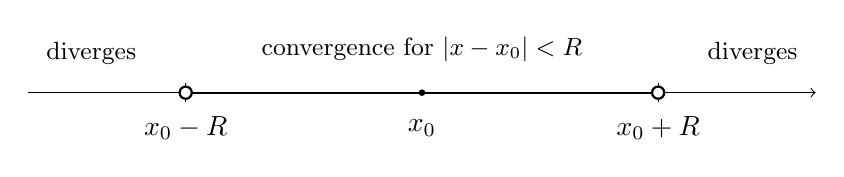
\begin{tikzpicture}
\draw[->] (-5,0) -- (5,0);
\node at (0,-0.45) {$x_0$};
\fill (0,0) circle (1.2pt);
\draw (-3,0.12) -- (-3,-0.12);
\draw (3,0.12) -- (3,-0.12);
\node at (-3,-0.45) {$x_0-R$};
\node at (3,-0.45) {$x_0+R$};
\draw[thick] (-3,0) -- (3,0);
\draw[white, line width=4pt] (-3,0) -- (-3,0); % keep endpoints visually clean
\draw[white, line width=4pt] (3,0) -- (3,0);
\draw[thick, fill=white] (-3,0) circle (2.2pt);
\draw[thick, fill=white] (3,0) circle (2.2pt);
\node at (0,0.55) {\small convergence for $|x-x_0|<R$};
\node at (-4.2,0.5) {\small diverges};
\node at (4.2,0.5) {\small diverges};
\end{tikzpicture}
\end{center}

% --- ADDED: practical computing R ---
\noindent\textbf{Computing $R$ in practice.}
Apply the ratio or root test to $\sum |c_n||x-x_0|^n$ and solve for $|x-x_0|$.
\begin{itemize}[leftmargin=*]
\item \textbf{Ratio test route:} Compute $L=\lim_{n\to\infty}\left|\frac{c_{n+1}}{c_n}\right|$. Then $R=1/L$ (with conventions $1/0=\infty$, $1/\infty=0$).
\item \textbf{Root test route:} Compute $A=\lim_{n\to\infty}\sqrt[n]{|c_n|}$. Then $R=1/A$.
\end{itemize}
Both methods give the same $R$ whenever both limits exist.
% --- END ADDED ---

\begin{examplebox}[title={Worked Example: finding $R$ and the interval (Lecture Ex.~6.3)}]
Find the radius and interval of convergence of $\displaystyle\sum_{n=1}^{\infty}\frac{(-1)^n}{(2n-1)\,2^n}(x-1)^n$.

\smallskip
\textbf{Step 1 (Ratio test).}
Let $a_n=\frac{(-1)^n}{(2n-1)\,2^n}(x-1)^n$. Then
\[
\left|\frac{a_{n+1}}{a_n}\right|
=\frac{2n-1}{2n+1}\cdot\frac{|x-1|}{2}
\xrightarrow[n\to\infty]{}\frac{|x-1|}{2}.
\]
Convergence when $\frac{|x-1|}{2}<1$, i.e.\ $|x-1|<2$, so $R=2$.

Endpoints:
\begin{itemize}[leftmargin=*]
\item At $x=3$: $(x-1)^n=2^n$, so the series becomes $\sum \frac{(-1)^n}{2n-1}$, which converges by the alternating series test.
\item At $x=-1$: $(x-1)^n=(-2)^n$, so the series becomes $\sum \frac{1}{2n-1}$, which diverges.
\end{itemize}
Therefore the interval of convergence is $(-1,\,3]$.
\end{examplebox}

% --- ADDED: extra worked example from lectures (Ex 6.4) ---
\begin{examplebox}[title={Worked Example: endpoint behaviour (Lecture Ex.~6.4)}]
Find $R$ and the interval of convergence for $\displaystyle\sum_{n=0}^{\infty}\frac{(-3)^n x^n}{\sqrt{n+1}}$.

\smallskip
\textbf{Step 1 (Ratio test).}
\[
\left|\frac{a_{n+1}}{a_n}\right|
=3|x|\,\sqrt{\frac{n+1}{n+2}}
\;\xrightarrow[n\to\infty]{}\;3|x|.
\]
Converges when $3|x|<1$, i.e.\ $|x|<\tfrac13$. So $R=\tfrac13$.

\textbf{Step 2 (Endpoints).}
\begin{itemize}[leftmargin=*]
\item $x=-\tfrac13$: series becomes $\sum \frac{1}{\sqrt{n+1}}$, which diverges ($p$-series, $p=\tfrac12<1$).
\item $x=\tfrac13$: series becomes $\sum \frac{(-1)^n}{\sqrt{n+1}}$, which converges (AST: $\frac{1}{\sqrt{n+1}}\downarrow 0$).
\end{itemize}
Interval of convergence: $\bigl(-\tfrac13,\,\tfrac13\bigr]$.
\end{examplebox}
% --- END ADDED ---

% --- ADDED: common mistake on endpoints ---
\begin{commonmistake}[title={Common Mistake: forgetting that endpoints can go either way}]
The ratio/root test is \emph{inconclusive} at $|x-x_0|=R$.
You must substitute each endpoint individually and apply a separate convergence test
(AST, $p$-series, comparison, $n$th-term test, \dots).
The four possible shapes $(\;),\;[\;),\;(\;],\;[\;]$ are all achievable.
\end{commonmistake}
% --- END ADDED ---

\begin{examtip}[title={Exam Focus: a fast workflow for $R$}]
\begin{enumerate}[leftmargin=*]
\item Identify the centre $x_0$ (from $(x-x_0)^n$).
\item Compute $R$ via ratio/root test \emph{ignoring} endpoints.
\item Test endpoints using quick divergence/alternating/comparison logic.
\item State both \textbf{radius} and \textbf{interval} clearly.
\end{enumerate}
\end{examtip}

% --- ADDED: extra exam tip on radius from singularity (Tutorial 12 Method 2) ---
\begin{examtip}[title={Exam Shortcut: radius from nearest singularity (Tutorial~12, Q1 Method~2)}]
For a Taylor series of an analytic function $f$ centred at $a$,
the radius of convergence equals the distance from $a$ to the \emph{nearest singularity}
(real or complex) of $f$.
\begin{itemize}[leftmargin=*]
\item $\ln x$ at $a=2$: singularity at $x=0$, so $R=|2-0|=2$.
\item $e^{2x}$ at $a=3$: entire function, so $R=\infty$.
\item $\sqrt{x}$ at $a=16$: branch point at $x=0$, so $R=|16-0|=16$.
\item $\frac{1}{7x-13}$ at $a=2$: pole at $x=\frac{13}{7}$, so $R=\left|2-\frac{13}{7}\right|=\frac{1}{7}$.
\end{itemize}
This is not a formal exam method (it relies on complex analysis) but is a powerful quick check.
\end{examtip}
% --- END ADDED ---

\subsection{Representing functions by power series (\S6.2)}

A major use-case is to rewrite a function into a form where a known power series applies, then transfer the convergence condition.

% --- ADDED: motivation paragraph ---
\noindent\textbf{The big idea.}
We already know one convergent power series by heart --- the geometric series.
The strategy of this entire section is:
\emph{start from the geometric series, then adapt it using algebra (substitution, multiplication) and calculus (term-by-term differentiation / integration) to represent new functions.}
Every example below follows this pattern.
% --- END ADDED ---

\begin{theorem}{Geometric series}{thm:geometric}
For $|x|<1$,
\[
\frac{1}{1-x}=\sum_{n=0}^{\infty}x^n.
\]
More generally, for constants $A\neq 0$ and $B$,
\[
\frac{1}{A-B(x-x_0)}=\frac{1}{A}\cdot \frac{1}{1-\frac{B}{A}(x-x_0)}
=\frac{1}{A}\sum_{n=0}^{\infty}\left(\frac{B}{A}\right)^n (x-x_0)^n,
\]
valid when $\left|\frac{B}{A}(x-x_0)\right|<1$.
\end{theorem}

% --- ADDED: step-by-step rewriting recipe ---
\noindent\textbf{Rewriting recipe (step by step).}
Given a rational function $\frac{C}{\alpha + \beta x}$:
\begin{enumerate}[leftmargin=*]
\item Factor out the constant from the denominator so you have $\frac{C}{\alpha}\cdot\frac{1}{1+\frac{\beta}{\alpha}x}$.
\item Recognise $\frac{1}{1+\frac{\beta}{\alpha}x}=\frac{1}{1-\bigl(-\frac{\beta}{\alpha}x\bigr)}$.
\item Apply the geometric series with $u=-\frac{\beta}{\alpha}x$.
\item The convergence condition is $|u|<1$, i.e.\ $|x|<\frac{|\alpha|}{|\beta|}$.
\end{enumerate}
% --- END ADDED ---

\begin{keyformula}[title={Key Formula: ``rewrite to geometric form'' pattern}]
Aim to express $f(x)$ as
\[
f(x)=\frac{C}{1-u(x)},
\quad\text{so that}\quad
f(x)=C\sum_{n=0}^{\infty}u(x)^n
\quad\text{when }|u(x)|<1.
\]
Then \textbf{the inequality $|u(x)|<1$ becomes your interval condition}.
\end{keyformula}

\begin{examplebox}[title={Worked Example: rational function to power series}]
Find a power series for $\displaystyle f(x)=\frac{3}{2+x}$ about $x_0=0$ and its interval of convergence.

Rewrite:
\[
\frac{3}{2+x}=\frac{3}{2}\cdot \frac{1}{1+\frac{x}{2}}
=\frac{3}{2}\cdot \frac{1}{1-\left(-\frac{x}{2}\right)}.
\]
Using Theorem~\ref{thm:geometric},
\[
\frac{3}{2+x}=\frac{3}{2}\sum_{n=0}^{\infty}\left(-\frac{x}{2}\right)^n
=\sum_{n=0}^{\infty} \frac{3(-1)^n}{2^{n+1}}x^n,
\]
valid when $\left|-\frac{x}{2}\right|<1$, i.e.\ $|x|<2$. Thus the radius is $R=2$.
\end{examplebox}

% --- ADDED: extra worked example with non-zero centre (Lecture Ex 6.7) ---
\begin{examplebox}[title={Worked Example: expansion about a non-zero centre (Lecture Ex.~6.7)}]
Find a power series representation of $\displaystyle\frac{1}{3x+1}$ at $x=1$.

\smallskip
Rewrite:
\[
\frac{1}{3x+1}=\frac{1}{3(x-1)+4}
=\frac{1}{4}\cdot\frac{1}{1-\bigl(-\tfrac{3}{4}(x-1)\bigr)}.
\]
For $\left|\tfrac{3}{4}(x-1)\right|<1$, i.e.\ $|x-1|<\tfrac{4}{3}$,
\[
\frac{1}{3x+1}
=\frac{1}{4}\sum_{n=0}^{\infty}\left(-\frac{3(x-1)}{4}\right)^n
=\sum_{n=0}^{\infty}\frac{(-1)^n 3^n}{4^{n+1}}(x-1)^n.
\]
The interval of convergence is $\bigl(-\tfrac13,\,\tfrac73\bigr)$ and $R=\tfrac43$.
\end{examplebox}
% --- END ADDED ---

% --- ADDED: worked example with higher powers (Lecture Ex 6.6) ---
\begin{examplebox}[title={Worked Example: substituting $u=-x^2$ (Lecture Ex.~6.6)}]
Express $\displaystyle f(x)=\frac{1}{1+x^2}$ as a power series and find its interval of convergence.

\smallskip
Replace $x$ by $-x^2$ in the geometric series:
\[
\frac{1}{1+x^2}=\frac{1}{1-(-x^2)}=\sum_{n=0}^{\infty}(-x^2)^n
=\sum_{n=0}^{\infty}(-1)^n x^{2n}.
\]
Convergence when $|-x^2|<1$, i.e.\ $|x|<1$. So $R=1$ and the interval is $(-1,1)$.

\smallskip
\textbf{Sanity check.}
At $n=0,1,2$: $1-x^2+x^4-\cdots$. Substituting $x=0$ gives $1=\frac{1}{1+0}$. \checkmark
\end{examplebox}
% --- END ADDED ---

\begin{commonmistake}[title={Common Mistake: losing the convergence condition}]
It is not enough to write down the series; you must also state where it is valid.
Always carry the condition $|u(x)|<1$ through your substitutions.
\end{commonmistake}

% --- ADDED: differentiation/integration to build new series ---
\noindent\textbf{Building new series via calculus.}
The term-by-term theorem (Theorem~\ref{thm:termwise} in \S6.3 below) lets us differentiate and integrate a known series to get a \emph{new} series with the \emph{same} radius $R$.
Two standard patterns:
\begin{itemize}[leftmargin=*]
\item \textbf{Differentiation:} $\frac{d}{dx}\frac{1}{1-x}=\frac{1}{(1-x)^2}=\sum_{n=1}^{\infty} n x^{n-1}$ for $|x|<1$.\\
Differentiating again: $\frac{2}{(1-x)^3}=\sum_{n=2}^{\infty}n(n-1)x^{n-2}$ for $|x|<1$.
\item \textbf{Integration:} $\int\frac{1}{1-x}\,dx=-\ln(1-x)=\sum_{n=1}^{\infty}\frac{x^n}{n}+C$ for $|x|<1$.\\
Setting $C=0$ (since $\ln 1=0$ at $x=0$) gives $\ln(1-x)=-\sum_{n=1}^{\infty}\frac{x^n}{n}$.
\end{itemize}

\begin{examplebox}[title={Worked Example: $\tan^{-1}x$ via integration (Lecture Ex.~6.10)}]
Prove that $\displaystyle\tan^{-1}x=\sum_{n=0}^{\infty}(-1)^n\frac{x^{2n+1}}{2n+1}$ for $|x|<1$.

\smallskip
Start from
$\frac{1}{1+x^2}=\sum_{n=0}^{\infty}(-1)^n x^{2n}$
(valid for $|x|<1$).
Integrate both sides from $0$ to $x$:
\[
\tan^{-1}x=\int_0^x \frac{1}{1+t^2}\,dt
=\sum_{n=0}^{\infty}(-1)^n\int_0^x t^{2n}\,dt
=\sum_{n=0}^{\infty}(-1)^n\frac{x^{2n+1}}{2n+1}.
\]
The constant of integration is zero because $\tan^{-1}0=0$.
The radius remains $R=1$ by Theorem~\ref{thm:termwise}.
\end{examplebox}
% --- END ADDED ---

% --- ADDED: extra worked example from Tutorial 11 Q5(b) ---
\begin{examplebox}[title={Worked Example: differentiating twice (Tutorial~11, Q5(b))}]
Find a power series for $\displaystyle\left(\frac{x}{2-x}\right)^3$ and its radius of convergence.

\smallskip
\textbf{Step 1.} Rewrite: $\left(\frac{x}{2-x}\right)^3=\frac{x^3}{8}\cdot\frac{1}{\left(1-\frac{x}{2}\right)^3}$.

\textbf{Step 2.} From $\frac{1}{1-u}=\sum u^n$, differentiate twice:
\[
\frac{2}{(1-u)^3}=\sum_{n=2}^{\infty}n(n-1)u^{n-2}
\quad\Longrightarrow\quad
\frac{1}{(1-u)^3}=\sum_{n=0}^{\infty}\binom{n+2}{2}u^n.
\]
\textbf{Step 3.} Substitute $u=x/2$ and multiply by $x^3/8$:
\[
\left(\frac{x}{2-x}\right)^3
=\sum_{n=0}^{\infty}\binom{n+2}{2}\frac{x^{n+3}}{2^{n+3}},
\qquad |x|<2.
\]
So $R=2$.
\end{examplebox}
% --- END ADDED ---

% --- ADDED: exam tip for section 6.2 ---
\begin{examtip}[title={Exam Focus: choosing the right manipulation}]
\begin{itemize}[leftmargin=*]
\item If $f$ has $\frac{1}{\text{linear in }x}$: use geometric series directly.
\item If $f$ has $\frac{1}{(\text{linear})^k}$: differentiate the geometric series $k-1$ times.
\item If $f$ involves $\ln$, $\tan^{-1}$: integrate the geometric series (after a substitution).
\item If $f$ has an extra $x^m$ factor: find the series for the rest, then multiply by $x^m$.
\end{itemize}
Always state the convergence condition after each manipulation.
\end{examtip}
% --- END ADDED ---

\subsection{Taylor and Maclaurin series (\S6.3)}

Power series become especially structured when the coefficients come from derivatives of a function.

\begin{definition}{Taylor polynomial and Taylor series}{def:taylor}
Let $f$ be $(n+1)$ times differentiable near $a$. The \emph{$n$th Taylor polynomial} of $f$ at $a$ is
\[
P_n(x)=\sum_{k=0}^{n}\frac{f^{(k)}(a)}{k!}(x-a)^k.
\]
If the infinite series converges, the \emph{Taylor series} of $f$ at $a$ is
\[
\sum_{k=0}^{\infty}\frac{f^{(k)}(a)}{k!}(x-a)^k.
\]
When $a=0$ this is called the \emph{Maclaurin series}.
\end{definition}

\noindent\textbf{Why these coefficients?}
A polynomial $P_n$ can be made to \emph{match $f$ and its derivatives at $a$} by enforcing
\[
P_n^{(k)}(a)=f^{(k)}(a)\quad (k=0,1,\dots,n).
\]
Solving these $n{+}1$ matching conditions yields exactly the coefficients $\frac{f^{(k)}(a)}{k!}$. In other words,
$P_n$ is the unique degree-$\le n$ polynomial that shares the same ``local data'' (value, slope, curvature, \dots) as $f$ at $a$.

% --- ADDED: detailed derivation of the coefficients ---
\noindent\textbf{Deriving the formula step by step (from the lecture notes).}
Suppose $f(x)=c_0+c_1(x-a)+c_2(x-a)^2+c_3(x-a)^3+\cdots$ for $|x-a|<R$.
\begin{itemize}[leftmargin=*]
\item Setting $x=a$: $f(a)=c_0$.
\item Differentiating once and setting $x=a$: $f'(a)=c_1$.
\item Differentiating twice and setting $x=a$: $f''(a)=2c_2$, so $c_2=\frac{f''(a)}{2!}$.
\item Differentiating three times and setting $x=a$: $f'''(a)=3!\,c_3$, so $c_3=\frac{f'''(a)}{3!}$.
\item In general: $f^{(n)}(a)=n!\,c_n$, giving $c_n=\frac{f^{(n)}(a)}{n!}$.
\end{itemize}
The factor $k!$ in the denominator arises because differentiating $(x-a)^k$ exactly $k$ times produces $k!$ (by the power rule applied repeatedly).
This is why the Taylor coefficient formula has $k!$ in the denominator --- it ``undoes'' the factorial that differentiation creates.
% --- END ADDED ---

\begin{theorem}{Taylor's theorem and remainder (Lagrange form)}{thm:taylor-remainder}
Assume $f$ has continuous derivatives up to order $n+1$ on an interval containing $a$ and $x$.
Then
\[
f(x)=P_n(x)+R_n(x),
\]
where $P_n$ is the $n$th Taylor polynomial at $a$, and there exists $c$ between $a$ and $x$ such that
\[
R_n(x)=\frac{f^{(n+1)}(c)}{(n+1)!}(x-a)^{n+1}.
\]
\end{theorem}

% --- ADDED: intuition for remainder and connection to FTC ---
\noindent\textbf{Why does the remainder look like that?}
Taylor's theorem is fundamentally an iterated application of the \textbf{Fundamental Theorem of Calculus} (FTC).
Here is the key idea:

\smallskip
\emph{Base case ($n=0$):} The FTC says
\[
f(x)-f(a)=\int_a^x f'(u)\,du.
\]
This is the remainder $R_0(x)=\int_a^x f'(u)\,du$ --- the difference between $f(x)$ and the $0$th Taylor polynomial $P_0(x)=f(a)$.

\smallskip
\emph{General case:} Repeating integration by parts gives the \emph{integral form} of the remainder:
\[
R_n(x)=\frac{1}{n!}\int_a^x (x-u)^n f^{(n+1)}(u)\,du.
\]
The Lagrange form then follows by applying the Mean Value Theorem for integrals:
since $(x-u)^n$ does not change sign on $[a,x]$, there exists some $c$ between $a$ and $x$ such that
\[
\frac{1}{n!}\int_a^x (x-u)^n f^{(n+1)}(u)\,du
=\frac{f^{(n+1)}(c)}{n!}\int_a^x (x-u)^n\,du
=\frac{f^{(n+1)}(c)}{(n+1)!}(x-a)^{n+1}.
\]

\smallskip
\noindent\textbf{Proof of the integral form via IBP (from lecture notes, Theorem 5).}
Define $I_n=\frac{1}{n!}\int_a^x (x-u)^n f^{(n+1)}(u)\,du$.
Use integration by parts with $U=\frac{(x-u)^n}{n!}$ and $V'=f^{(n+1)}(u)$:
\[
I_n = \biggl[\frac{(x-u)^n}{n!}f^{(n)}(u)\biggr]_a^x + \frac{1}{(n-1)!}\int_a^x (x-u)^{n-1}f^{(n)}(u)\,du
= -\frac{f^{(n)}(a)}{n!}(x-a)^n + I_{n-1}.
\]
Rearranging: $I_{n-1}=\frac{f^{(n)}(a)}{n!}(x-a)^n + I_n$.
Applying this recurrence $n$ times starting from $f(x)=f(a)+I_0$ yields
\[
f(x)=\underbrace{f(a)+f'(a)(x-a)+\cdots+\frac{f^{(n)}(a)}{n!}(x-a)^n}_{P_n(x)}+I_n,
\]
proving $R_n(x)=I_n$.
% --- END ADDED ---

\begin{keyformula}[title={Key Formula: Error bound for Taylor approximation}]
If $|f^{(n+1)}(t)|\le M$ for all $t$ between $a$ and $x$, then
\[
|R_n(x)|\le \frac{M}{(n+1)!}\,|x-a|^{n+1}.
\]
This is the standard tool to prove $R_n(x)\to 0$ as $n\to\infty$ for a fixed $x$.
\end{keyformula}

% --- ADDED: why factorial dominates ---
\noindent\textbf{Why $\frac{|x-a|^{n+1}}{(n+1)!}\to 0$ always.}
This fact, used in almost every ``prove Taylor series equals $f$'' problem, deserves a short justification.
Fix any real number $r=|x-a|$. For $n\ge 2r$, each new factor satisfies
$\frac{r}{n+1}\le \frac{r}{2r+1}<\frac{1}{2}$.
So beyond that point, multiplying by $\frac{r}{n+1}$ halves the term each time, driving it to $0$.
More precisely, $\frac{r^{n+1}}{(n+1)!}\le \frac{r^{\lceil 2r\rceil}}{\lceil 2r\rceil!}\cdot\bigl(\tfrac12\bigr)^{n+1-\lceil 2r\rceil}\to 0$.
% --- END ADDED ---

\begin{theorem}{When a Taylor series equals the function}{thm:taylor-equals}
If $\lim\limits_{n\to\infty} R_n(x)=0$ for a given $x$, then
\[
f(x)=\sum_{k=0}^{\infty}\frac{f^{(k)}(a)}{k!}(x-a)^k
\]
at that $x$. If this holds for all $x$ in an interval, then the Taylor series represents $f$ on that interval.
\end{theorem}

% --- ADDED: full worked proof for e^x ---
\begin{examplebox}[title={Worked Example: proving $e^x$ equals its Maclaurin series (Lecture Ex.~6.12)}]
\textbf{Step 1 (Series).} Since $f^{(n)}(x)=e^x$ for all $n$, we have $f^{(n)}(0)=1$, giving the Maclaurin series
$\sum_{n=0}^{\infty}\frac{x^n}{n!}$ with $R=\infty$ (by ratio test).

\smallskip
\textbf{Step 2 (Remainder $\to 0$).}
Pick any $d>0$. For $|x|\le d$, we have $|f^{(n+1)}(t)|=e^t\le e^d$. So
\[
|R_n(x)|\le \frac{e^d}{(n+1)!}|x|^{n+1}\to 0
\quad\text{as }n\to\infty.
\]
Since $d$ is arbitrary, $R_n(x)\to 0$ for \emph{all} $x\in\mathbb{R}$.

\smallskip
\textbf{Conclusion.} By Theorem~\ref{thm:taylor-equals},
$e^x=\sum_{n=0}^{\infty}\frac{x^n}{n!}$ for all $x$.
\end{examplebox}
% --- END ADDED ---

\begin{examplebox}[title={Worked Example: Maclaurin series for $\sin x$ and $\cos x$}]
Using derivatives of $\sin x$:
\[
\sin x,\quad \cos x,\quad -\sin x,\quad -\cos x,\quad \sin x,\ \dots
\]
At $x=0$:
\[
\sin 0=0,\ \cos 0=1,\ -\sin 0=0,\ -\cos 0=-1,\ \dots
\]
Hence the Maclaurin series is
\[
\sin x=\sum_{n=0}^{\infty}(-1)^n\frac{x^{2n+1}}{(2n+1)!}
= x-\frac{x^3}{3!}+\frac{x^5}{5!}-\cdots \qquad (R=\infty).
\]
Term-by-term differentiation (justified by Theorem~\ref{thm:termwise} below) yields
\[
\cos x=\sum_{n=0}^{\infty}(-1)^n\frac{x^{2n}}{(2n)!}
=1-\frac{x^2}{2!}+\frac{x^4}{4!}-\cdots \qquad (R=\infty).
\]
\end{examplebox}

% --- ADDED: proving sin x equals its series ---
\noindent\textbf{Proving $\sin x$ equals its Maclaurin series (Lecture Ex.~6.13).}
Since $f^{(n+1)}(x)=\pm\sin x$ or $\pm\cos x$, we have $|f^{(n+1)}(x)|\le 1$ for all $x$.
The error bound gives $|R_n(x)|\le \frac{|x|^{n+1}}{(n+1)!}\to 0$.
By the Squeeze Theorem, $R_n(x)\to 0$ for all $x$, so the Maclaurin series represents $\sin x$ on all of $\mathbb{R}$.
The same argument applies to $\cos x$ (or use term-by-term differentiation of the $\sin x$ series).
% --- END ADDED ---

\begin{commonmistake}[title={Common Mistake: ``Taylor series exists'' vs ``Taylor series equals $f$''}]
Writing down $\sum \frac{f^{(k)}(a)}{k!}(x-a)^k$ does \emph{not} automatically mean it equals $f(x)$.
You must either:
\begin{itemize}[leftmargin=*]
\item use Theorem~\ref{thm:taylor-equals} by showing $R_n(x)\to 0$ (often via the error bound), or
\item identify it with a known series representation (e.g.\ reduce to $\sin$, $\cos$, $e^x$, geometric).
\end{itemize}
\end{commonmistake}

\begin{examtip}[title={Exam Focus: proving $R_n(x)\to 0$ quickly}]
A standard pattern is:
\begin{itemize}[leftmargin=*]
\item bound $|f^{(n+1)}(t)|\le M$ by a constant (often $1$, $e^{|t|}$, or a simple maximum);
\item apply $|R_n(x)|\le \frac{M}{(n+1)!}|x-a|^{n+1}$;
\item conclude $\frac{|x-a|^{n+1}}{(n+1)!}\to 0$ as $n\to\infty$ (factorial dominates powers).
\end{itemize}
\end{examtip}

% --- ADDED: Taylor series at nonzero centre via substitution (Tutorial 12 Q1) ---
\begin{examplebox}[title={Worked Example: Taylor series at $a\neq 0$ via substitution (Tutorial~12, Q1(a))}]
Find the Taylor series for $\ln x$ centred at $a=2$.

\smallskip
\textbf{Key idea:} reduce to a known Maclaurin series by substitution.
Write $x=2+(x-2)$, so
\[
\ln x = \ln\bigl(2+(x-2)\bigr) = \ln 2 + \ln\!\left(1+\frac{x-2}{2}\right).
\]
Let $u=\frac{x-2}{2}$. Using $\ln(1+u)=\sum_{n=1}^{\infty}(-1)^{n+1}\frac{u^n}{n}$ for $|u|<1$:
\[
\ln x = \ln 2 + \sum_{n=1}^{\infty}(-1)^{n+1}\frac{(x-2)^n}{n\cdot 2^n},
\qquad |x-2|<2.
\]
So $R=2$. (Alternatively: nearest singularity of $\ln x$ is $x=0$, distance $|2-0|=2$.)

\smallskip
\textbf{Exam tip.} The substitution method (reduce to a known Maclaurin series) is almost always faster than computing $f^{(n)}(a)/n!$ by hand, especially for $\ln$, $e^x$, and trig functions.
\end{examplebox}
% --- END ADDED ---

% --- ADDED: first few nonzero terms via multiplication (Tutorial 12 Q3) ---
\begin{examplebox}[title={Worked Example: first three nonzero Maclaurin terms (Tutorial~12, Q3)}]
Find the first three nonzero terms of the Maclaurin series for:

\smallskip
\textbf{(a) $\sec x$.}
Since $\sec x$ is even, write $\sec x=1+Ax^2+Bx^4+O(x^6)$.
Use $(\sec x)(\cos x)=1$ and $\cos x=1-\frac{x^2}{2}+\frac{x^4}{24}+O(x^6)$:
\[
(1+Ax^2+Bx^4)\!\left(1-\frac{x^2}{2}+\frac{x^4}{24}\right)=1.
\]
Matching $x^2$: $A-\frac12=0\Rightarrow A=\frac12$.
Matching $x^4$: $B-\frac{A}{2}+\frac{1}{24}=0\Rightarrow B=\frac{5}{24}$.
So $\sec x=1+\frac{x^2}{2}+\frac{5x^4}{24}+O(x^6)$.

\smallskip
\textbf{(b) $e^x\ln(1+x)$.}
Multiply truncated series:
$e^x=1+x+\frac{x^2}{2}+\frac{x^3}{6}+O(x^4)$ and $\ln(1+x)=x-\frac{x^2}{2}+\frac{x^3}{3}+O(x^4)$.
Collecting:
$e^x\ln(1+x)=x+\frac{x^2}{2}+\frac{x^3}{3}+O(x^4)$.
\end{examplebox}
% --- END ADDED ---

\begin{theorem}{Term-by-term differentiation/integration of power series}{thm:termwise}
Let $\sum_{n=0}^{\infty} c_n (x-x_0)^n$ have radius of convergence $R>0$.
For $|x-x_0|<R$:
\begin{enumerate}[leftmargin=*]
\item (Differentiation) $\displaystyle\frac{d}{dx}\sum_{n=0}^{\infty}c_n(x-x_0)^n=\sum_{n=1}^{\infty}nc_n(x-x_0)^{n-1}$, with the same radius $R$.
\item (Integration) $\displaystyle\int\sum_{n=0}^{\infty}c_n(x-x_0)^n\,dx=C+\sum_{n=0}^{\infty}\frac{c_n}{n+1}(x-x_0)^{n+1}$, with the same radius $R$.
\end{enumerate}
\end{theorem}

% --- ADDED: emphasis on why same R ---
\noindent\textbf{Why does the radius stay the same?}
Differentiation multiplies the $n$th coefficient by $n$, and integration divides it by $n+1$.
Neither operation changes the growth rate of $|c_n|$ fast enough to alter $R=1/\limsup\sqrt[n]{|c_n|}$.
(Formally: $\sqrt[n]{n}\to 1$, so $\limsup\sqrt[n]{n|c_n|}=\limsup\sqrt[n]{|c_n|}$.)

\noindent\textbf{Important caveat.}
The radius $R$ is preserved, but endpoint convergence may change.
For example, $\sum \frac{x^n}{n}$ converges at $x=-1$, but its derivative $\sum x^{n-1}$ (the geometric series) diverges at $x=-1$.
Always re-check endpoints after differentiation or integration.
% --- END ADDED ---

% --- ADDED: reference table of important Maclaurin series ---
\begin{keyformula}[title={Key Formula: Important Maclaurin series (memorise for exams)}]
\[
\renewcommand{\arraystretch}{1.6}
\begin{array}{lll}
\toprule
\textbf{Function} & \textbf{Maclaurin series} & \textbf{Radius}\\
\midrule
\dfrac{1}{1-x} & \displaystyle\sum_{n=0}^{\infty}x^n & R=1\\[4pt]
e^x & \displaystyle\sum_{n=0}^{\infty}\dfrac{x^n}{n!} & R=\infty\\[4pt]
\sin x & \displaystyle\sum_{n=0}^{\infty}(-1)^n\dfrac{x^{2n+1}}{(2n+1)!} & R=\infty\\[4pt]
\cos x & \displaystyle\sum_{n=0}^{\infty}(-1)^n\dfrac{x^{2n}}{(2n)!} & R=\infty\\[4pt]
\tan^{-1}x & \displaystyle\sum_{n=0}^{\infty}(-1)^n\dfrac{x^{2n+1}}{2n+1} & R=1\\[4pt]
\ln(1+x) & \displaystyle\sum_{n=1}^{\infty}(-1)^{n-1}\dfrac{x^n}{n} & R=1\\[4pt]
(1+x)^k & \displaystyle\sum_{n=0}^{\infty}\binom{k}{n}x^n & R=1\\
\bottomrule
\end{array}
\]
\end{keyformula}
% --- END ADDED ---

\subsection{The binomial series (\S6.4)}

% --- ADDED: motivation ---
\noindent\textbf{Motivation.}
The classical Binomial Theorem $(a+b)^n=\sum_{i=0}^{n}\binom{n}{i}a^{n-i}b^i$ works only when $n$ is a \emph{non-negative integer} (the sum is finite).
What if $n$ is a fraction like $\frac12$ (for square roots) or a negative integer like $-1$ (for reciprocals)?
The \emph{binomial series} answers this: it extends the expansion to \emph{any} real exponent $k$, at the price of becoming an infinite series that converges only for $|x|<1$.
% --- END ADDED ---

\begin{definition}{Generalised binomial coefficient}{def:gen-binom}
For any real $k$ and non-negative integer $n\ge 1$,
\[
\binom{k}{n}=\frac{k(k-1)(k-2)\cdots(k-n+1)}{n!}.
\]
By convention $\binom{k}{0}=1$.
When $k$ is a positive integer, this reduces to the usual $\frac{k!}{n!(k-n)!}$.
\end{definition}

% --- ADDED: why the generalised coefficient works ---
\noindent\textbf{Why this definition?}
The standard binomial coefficient $\binom{n}{i}=\frac{n!}{i!(n-i)!}$ only makes sense when $n$ is a non-negative integer (because of the factorials).
The ``falling factorial'' form $\frac{k(k-1)\cdots(k-n+1)}{n!}$ makes sense for \emph{any} real $k$, because it only involves $n$ factors in the numerator.
When $k$ is a positive integer and $n>k$, one of the factors in the numerator is zero, so $\binom{k}{n}=0$ and the series terminates (recovering the classical theorem).
For non-integer $k$, none of these factors is ever zero, so the series is genuinely infinite.
% --- END ADDED ---

\begin{theorem}{The binomial series}{thm:binomial}
If $k$ is any real number and $|x|<1$, then
\[
(1+x)^k = \sum_{n=0}^{\infty}\binom{k}{n}x^n.
\]
The radius of convergence is $R=1$ (when $k$ is not a non-negative integer).
\end{theorem}

% --- ADDED: proof sketch of R=1 via ratio test ---
\noindent\textbf{Why $R=1$?}
Let $a_n=\binom{k}{n}x^n$. The ratio test gives
\[
\left|\frac{a_{n+1}}{a_n}\right|
=\frac{|k-n|}{n+1}|x|
=\frac{|1-k/n|}{1+1/n}|x|
\;\xrightarrow[n\to\infty]{}\;|x|.
\]
So the series converges when $|x|<1$ and diverges when $|x|>1$, giving $R=1$.
Convergence at $x=\pm 1$ depends on the specific value of $k$.
% --- END ADDED ---

\begin{examplebox}[title={Worked Example: binomial series for $1/\sqrt{4-x}$ (Lecture Ex.~6.18)}]
Rewrite:
\[
\frac{1}{\sqrt{4-x}}=\frac{1}{2}\left(1-\frac{x}{4}\right)^{-1/2}.
\]
Apply the binomial series with $k=-\frac12$ and substitute $x\mapsto -\frac{x}{4}$:
\[
\frac{1}{\sqrt{4-x}}
=\frac{1}{2}\sum_{n=0}^{\infty}\binom{-1/2}{n}\left(-\frac{x}{4}\right)^n,
\qquad |x|<4.
\]
Using $\binom{-1/2}{n}=\frac{(-1)^n\cdot 1\cdot 3\cdot 5\cdots(2n-1)}{2^n\,n!}$, the series simplifies to
\[
\frac{1}{\sqrt{4-x}}=\frac{1}{2}+\frac{1}{2}\sum_{n=1}^{\infty}\frac{1\cdot 3\cdot 5\cdots(2n-1)}{n!\,8^n}x^n,
\qquad R=4.
\]
\end{examplebox}

% --- ADDED: extra worked example from Tutorial 12 Q5 ---
\begin{examplebox}[title={Worked Example: cube root (Tutorial~12, Q5)}]
Find the Maclaurin series for $f(x)=\sqrt[3]{8+x}$ and its radius of convergence.

\smallskip
Rewrite: $(8+x)^{1/3}=2\bigl(1+\frac{x}{8}\bigr)^{1/3}$.
Apply binomial series with $k=\frac13$ and $u=\frac{x}{8}$:
\[
\sqrt[3]{8+x}=2\sum_{n=0}^{\infty}\binom{1/3}{n}\left(\frac{x}{8}\right)^n,
\qquad |x|<8.
\]
Explicitly:
\[
\sqrt[3]{8+x}=2+\frac{x}{12}-\frac{x^2}{288}+\frac{5x^3}{20736}+\cdots
\]
The radius is $R=8$ (the substitution $u=x/8$ requires $|u|<1$, i.e.\ $|x|<8$).
\end{examplebox}
% --- END ADDED ---

% --- ADDED: common mistake for binomial series ---
\begin{commonmistake}[title={Common Mistake: wrong form for binomial series}]
The binomial series applies to $(1+x)^k$, \textbf{not} $(a+x)^k$ directly.
You must first factor out the constant:
\[
(a+x)^k = a^k\left(1+\frac{x}{a}\right)^k,
\]
then apply the series with $u=x/a$. The convergence condition becomes $|x/a|<1$, i.e.\ $|x|<|a|$.
\end{commonmistake}
% --- END ADDED ---

% --- ADDED: exam tip for binomial series ---
\begin{examtip}[title={Exam Focus: when to use the binomial series}]
Use the binomial series when you see:
\begin{itemize}[leftmargin=*]
\item Square roots: $\sqrt{1+x}=(1+x)^{1/2}$, $\frac{1}{\sqrt{1+x}}=(1+x)^{-1/2}$.
\item Cube roots: $\sqrt[3]{1+x}=(1+x)^{1/3}$.
\item Negative integer powers: $\frac{1}{(1+x)^2}=(1+x)^{-2}$.
\end{itemize}
Always rewrite into the form $(1+u)^k$ first, then state $|u|<1$.
\end{examtip}
% --- END ADDED ---

\subsection{Finding limits using power series (\S6.5)}

% --- ADDED: motivation ---
\noindent\textbf{Why use power series for limits?}
Some limits of the form $\lim_{x\to 0}\frac{f(x)}{g(x)}$ are $0/0$ indeterminate forms that would require multiple rounds of L'H\^{o}pital's rule.
Power series provide a faster alternative:
expand numerator and denominator, cancel the leading power of $x$, and read off the limit directly.
This is especially efficient when the Maclaurin series are already known.
% --- END ADDED ---

% --- ADDED: method box ---
\begin{keyformula}[title={Key Formula: series limit technique}]
To evaluate $\lim_{x\to 0}\frac{f(x)}{g(x)}$ (a $0/0$ form):
\begin{enumerate}[leftmargin=*]
\item Replace $f(x)$ and $g(x)$ by their Maclaurin series (keep enough terms).
\item Cancel the lowest common power of $x$ from numerator and denominator.
\item Set $x=0$ in what remains.
\end{enumerate}
The number of terms you need equals the number of cancellations plus one.
\end{keyformula}
% --- END ADDED ---

\begin{examplebox}[title={Worked Example: series limit (Lecture Ex.~6.20)}]
Evaluate $\displaystyle\lim_{x\to 0}\frac{e^x-1-x}{x^2}$.

\smallskip
Expand: $e^x=1+x+\frac{x^2}{2!}+\frac{x^3}{3!}+\cdots$.
Then
\[
\frac{e^x-1-x}{x^2}=\frac{\frac{x^2}{2!}+\frac{x^3}{3!}+\cdots}{x^2}
=\frac{1}{2}+\frac{x}{6}+\cdots\;\xrightarrow[x\to 0]{}\;\frac{1}{2}.
\]
\end{examplebox}

% --- ADDED: worked example from Tutorial 12 Q4 ---
\begin{examplebox}[title={Worked Example: series limit with $\ln$ (Tutorial~12, Q4(a))}]
Evaluate $\displaystyle\lim_{x\to 0}\frac{2x-\ln(1+2x)}{x^2}$.

\smallskip
Use $\ln(1+u)=u-\frac{u^2}{2}+\frac{u^3}{3}+O(u^4)$ with $u=2x$:
\[
\ln(1+2x)=2x-2x^2+\tfrac{8}{3}x^3+O(x^4).
\]
Then
\[
2x-\ln(1+2x)=2x^2-\tfrac{8}{3}x^3+O(x^4),
\]
so
\[
\frac{2x-\ln(1+2x)}{x^2}=2-\tfrac{8}{3}x+O(x^2)\;\xrightarrow[x\to 0]{}\;2.
\]
\end{examplebox}
% --- END ADDED ---

% --- ADDED: worked example with binomial series from Tutorial 12 Q4(b) ---
\begin{examplebox}[title={Worked Example: binomial series limit (Tutorial~12, Q4(b))}]
Evaluate $\displaystyle\lim_{x\to 0}\frac{\sqrt{1+x}-1-\frac12 x}{x^2}$.

\smallskip
Use $(1+x)^{1/2}=1+\frac12 x-\frac18 x^2+O(x^3)$.
Then
\[
\sqrt{1+x}-1-\tfrac12 x=-\tfrac18 x^2+O(x^3),
\]
so the limit is $-\frac18$.
\end{examplebox}
% --- END ADDED ---

% --- ADDED: lecture example 6.21 ---
\begin{examplebox}[title={Worked Example: $\lim_{x\to 0}\frac{1-\cos x}{1+x-e^x}$ (Lecture Ex.~6.21)}]
Expand:
\begin{align*}
1-\cos x &= \frac{x^2}{2}-\frac{x^4}{24}+\cdots,\\
1+x-e^x &= 1+x-\left(1+x+\frac{x^2}{2}+\frac{x^3}{6}+\cdots\right)
=-\frac{x^2}{2}-\frac{x^3}{6}-\cdots.
\end{align*}
Divide:
\[
\frac{1-\cos x}{1+x-e^x}
=\frac{\frac{x^2}{2}+O(x^4)}{-\frac{x^2}{2}+O(x^3)}
=\frac{\frac12+O(x^2)}{-\frac12+O(x)}
\;\xrightarrow[x\to 0]{}\;\frac{1/2}{-1/2}=-1.
\]
\end{examplebox}
% --- END ADDED ---

% --- ADDED: summing series via recognition ---
\noindent\textbf{Summing numerical series by recognising a power series.}
A common exam question gives you a numerical series and asks you to find its sum.
The technique: identify the series as a known power series evaluated at a specific $x$.

\begin{examplebox}[title={Worked Example: summing via standard series (Tutorial~12, Q6)}]
\textbf{(a)} Find $\displaystyle\sum_{n=0}^{\infty}(-1)^n\frac{\pi^{2n+1}}{4^{2n+1}(2n+1)!}$.

This is $\sum_{n=0}^{\infty}(-1)^n\frac{z^{2n+1}}{(2n+1)!}$ with $z=\pi/4$, which equals $\sin(\pi/4)=\frac{1}{\sqrt{2}}$.

\smallskip
\textbf{(b)} Find $\displaystyle\frac{1}{1\cdot 2}-\frac{1}{3\cdot 2^3}+\frac{1}{5\cdot 2^5}-\cdots$.

Write it as $\sum_{n=0}^{\infty}(-1)^n\frac{(1/2)^{2n+1}}{2n+1}=\tan^{-1}(1/2)$.
\end{examplebox}
% --- END ADDED ---

% --- ADDED: summing via differentiation (Tutorial 11 Q6(b)) ---
\begin{examplebox}[title={Worked Example: $\sum n(n-1)/2^n$ via generating function (Tutorial~11, Q6(b))}]
Find $\displaystyle\sum_{n=2}^{\infty}\frac{n(n-1)}{2^n}$.

\smallskip
\textbf{Step 1.} From $\frac{1}{1-x}=\sum x^n$, differentiate twice:
$\frac{2}{(1-x)^3}=\sum_{n=2}^{\infty}n(n-1)x^{n-2}$.

\textbf{Step 2.} Multiply by $x^2$:
$\frac{2x^2}{(1-x)^3}=\sum_{n=2}^{\infty}n(n-1)x^n$.

\textbf{Step 3.} Substitute $x=\frac12$:
$\frac{2\cdot(1/4)}{(1/2)^3}=\frac{1/2}{1/8}=4$.
\end{examplebox}
% --- END ADDED ---

\begin{examtip}[title={Exam Focus: series limits vs L'H\^{o}pital}]
\begin{itemize}[leftmargin=*]
\item Use series when you know the Maclaurin expansions and the limit involves $x\to 0$.
For $x\to a\neq 0$, substitute $h=x-a$ and expand in $h$.
\item Use L'H\^{o}pital when the function does not have a convenient series expansion.
\item Both methods can verify each other; in exams, series is usually faster.
\end{itemize}
\end{examtip}

% --- ADDED: Fibonacci generating function from Tutorial 12 Q8 ---
\begin{extension}[title={Extension (Beyond Syllabus: Fibonacci generating function --- Tutorial~12, Q8)}]
\textbf{Syllabus link:} Chapter 6 --- \S6.2 Representing Functions by Power Series.\smallskip\\
The function $f(x)=\frac{x}{1-x-x^2}$ has Maclaurin series $\sum_{n=1}^{\infty}f_n x^n$, where $f_n$ is the $n$th Fibonacci number ($f_1=f_2=1$, $f_n=f_{n-1}+f_{n-2}$).

\smallskip
\textbf{Proof.} Assume $f(x)=\sum_{n=1}^{\infty}a_n x^n$.
From $(1-x-x^2)f(x)=x$, equate coefficients:
$a_1=1$, $a_2-a_1=0$ (so $a_2=1$), and for $n\ge 3$: $a_n-a_{n-1}-a_{n-2}=0$.
This is exactly the Fibonacci recurrence.

\smallskip
\textbf{Binet formula.} Factor $1-x-x^2=-(x-\alpha)(x-\beta)$ where $\alpha=\frac{-1+\sqrt5}{2}$, $\beta=\frac{-1-\sqrt5}{2}$.
Partial fractions give $f(x)=\frac{1}{\sqrt5}\bigl(\frac{1}{1-x/\alpha^{-1}}-\frac{1}{1-x/\beta^{-1}}\bigr)$.
Expanding as geometric series and comparing yields the Binet formula:
\[
f_n=\frac{1}{\sqrt5}\left(\varphi^n-\psi^n\right),
\qquad \varphi=\frac{1+\sqrt5}{2},\;\psi=\frac{1-\sqrt5}{2}.
\]
\end{extension}
% --- END ADDED ---

\begin{extension}[title={Extension (Beyond Syllabus: coefficient-ratio formula for $R$ --- Tutorial~11, Q2)}]
\textbf{Syllabus link:} Chapter 6 --- \S6.1 Power Series (Radius of Convergence).\\
\textbf{Theorem.} Suppose $\sum_{n=0}^{\infty} c_n(x-a)^n$ satisfies $c_n\neq 0$ for all $n$, and $L=\lim_{n\to\infty}\left|\frac{c_n}{c_{n+1}}\right|$ exists. Then $R=L$.

\smallskip
\textbf{Proof sketch.}
Fix $x\neq a$ and set $u_n=|c_n|\,|x-a|^n>0$. Then
\[
\frac{u_{n+1}}{u_n}=\frac{|c_{n+1}|}{|c_n|}\,|x-a|\to\frac{|x-a|}{L}.
\]
By the ratio test:
\begin{itemize}[leftmargin=*]
\item if $|x-a|<L$, then $\frac{|x-a|}{L}<1$, so $\sum u_n$ converges and thus $\sum c_n(x-a)^n$ converges absolutely;
\item if $|x-a|>L$, then $\frac{|x-a|}{L}>1$, so $\sum u_n$ diverges and thus $\sum c_n(x-a)^n$ diverges.
\end{itemize}
Therefore the radius of convergence is $R=L$.

\smallskip
\textbf{Why this matters (exam-safe).} This gives a one-line radius computation when $\left|\frac{c_n}{c_{n+1}}\right|$ has a clean limit, avoiding repeated ratio/root test algebra.
\end{extension}

\begin{extension}[title={Extension (Beyond Syllabus: Cauchy--Hadamard radius formula)}]
\textbf{Syllabus link:} Chapter 6 --- \S6.1 Power Series (Radius of Convergence).\\
\textbf{Theorem (Cauchy--Hadamard).} For $\sum_{n=0}^{\infty} c_n (x-x_0)^n$, define
\[
A:=\limsup_{n\to\infty}\sqrt[n]{|c_n|}\in[0,\infty].
\]
Then the radius of convergence is
\[
R=\frac{1}{A}
\quad (\text{with }1/0=\infty,\ 1/\infty=0).
\]

\smallskip
\textbf{Proof (full working).}
Fix $x$ and set $r=|x-x_0|$. Consider $a_n=|c_n|r^n\ge 0$.
Then
\[
\limsup_{n\to\infty}\sqrt[n]{a_n}
=\limsup_{n\to\infty}\bigl(\sqrt[n]{|c_n|}\,r\bigr)
=r\cdot \limsup_{n\to\infty}\sqrt[n]{|c_n|}
=rA.
\]
By the root test:
\begin{itemize}[leftmargin=*]
\item if $rA<1$, i.e.\ $r<\frac{1}{A}$, then $\sum a_n$ converges, hence the power series converges absolutely;
\item if $rA>1$, i.e.\ $r>\frac{1}{A}$, then $\sum a_n$ diverges, hence the power series diverges.
\end{itemize}
Thus the radius is $R=1/A$.

\smallskip
\textbf{Why this matters (exam-safe).} It packages the radius computation into a single $\limsup$, and it explains why ratio/root tests lead to the same $R$.
\end{extension}

\begin{extension}[title={Extension (Beyond Syllabus: uniqueness of power series coefficients)}]
\textbf{Syllabus link:} Chapter 6 --- \S6.3 Taylor \& Maclaurin Series (Power series representation).\\
\textbf{Proposition.} Suppose $\sum_{n=0}^{\infty} c_n (x-a)^n$ converges for $|x-a|<R$ with $R>0$, and
\[
\sum_{n=0}^{\infty} c_n (x-a)^n = 0 \quad \text{for all } |x-a|<R.
\]
Then $c_n=0$ for all $n\ge 0$.

\smallskip
\textbf{Proof (inductive).}
Setting $x=a$ gives $c_0=0$.
Subtracting $c_0$ and dividing by $(x-a)$: $\sum_{n=1}^{\infty}c_n(x-a)^{n-1}=0$ for $0<|x-a|<R$.
By continuity of power series the sum is also $0$ at $x=a$, giving $c_1=0$.
Repeating yields $c_n=0$ for all $n$.

\smallskip
\textbf{Why this matters.} It guarantees that the Taylor series of $f$ at $a$ is the \emph{only} power series representation of $f$ near $a$.
If you find \emph{any} power series equal to $f$, its coefficients must be $\frac{f^{(n)}(a)}{n!}$.
This is why the substitution method (e.g.\ reducing $\ln x$ to $\ln(1+u)$) and the direct derivative method must give the same answer.
\end{extension}

% --- ADDED: extension for radius under substitution (Tutorial 11 Q3) ---
\begin{extension}[title={Extension (Beyond Syllabus: radius under $x\mapsto x^2$ --- Tutorial~11, Q3)}]
\textbf{Syllabus link:} Chapter 6 --- \S6.1 Power Series (Radius of Convergence).\smallskip\\
\textbf{Proposition.} If $\sum c_n x^n$ has radius $R$, then $\sum c_n x^{2n}$ has radius $\sqrt{R}$.

\smallskip
\textbf{Proof.}
Let $y=x^2$. Then $\sum c_n x^{2n}=\sum c_n y^n$, which converges iff $|y|<R$, i.e.\ $|x^2|<R$, i.e.\ $|x|<\sqrt{R}$.
\end{extension}
% --- END ADDED ---

%==================================================
% USER COMMENTS (EDITABLE)
%==================================================
% add explanantion to the ftc part especially, avoid giving the definitons directly without any explanaitoin on why are they like that
%
% DONE: Added extensive motivation for Taylor's remainder, including:
%   - Base case from FTC: f(x)-f(a) = int f'(u) du
%   - Integral form of remainder via repeated IBP
%   - How Lagrange form follows from MVT for integrals
%   - Full IBP recurrence proof from lecture notes (Theorem 5)
%   - Explanation of why factorial dominates powers
%
% Also added throughout:
%   - "Why these coefficients?" derivation step by step
%   - "Why three cases?" for radius of convergence
%   - "Why generalised binomial coefficient?" explanation
%   - "Why same R under differentiation?" explanation
%   - Motivation paragraphs before each major section
%   - Multiple tutorial-sourced examples (T11 Q5b, Q6b; T12 Q1a, Q3, Q4, Q5, Q6, Q8)
%==================================================

\newpage


\appendix
%==================================================
\section{Special Techniques}

\subsection{Symmetry and transformation tricks}
\subsubsection{Finite-interval reflection and averaging}
For any integrable \(f\) on \([a,b]\),
\[
\int_a^b f(x)\,dx=\int_a^b f(a+b-x)\,dx,
\qquad
\int_a^b f(x)\,dx=\frac12\int_a^b\!\bigl(f(x)+f(a+b-x)\bigr)\,dx.
\]

\paragraph{Intuition.}
Pair each point \(x\) with its mirror image \(a+b-x\) about the midpoint of the interval.

\paragraph{How it works.}
The substitution \(u=a+b-x\) preserves the interval \([a,b]\). In many problems, the reflected integrand complements the original one, and averaging the two forms simplifies the algebra dramatically.

\paragraph{Why it is useful.}
Many difficult definite integrals are not meant to be attacked by antiderivatives. Reflection often converts the problem into a one-line identity.

\paragraph{When to try this.}
Use it when the interval is finite and the integrand contains both \(x\) and \(a+b-x\), or when expressions in \(x\) and \(1-x\) naturally appear together.

\paragraph{Worked example.}
Let
\[
I=\int_0^1 \frac{x^2}{x^2+(1-x)^2}\,dx.
\]
Reflecting \(x\mapsto 1-x\),
\[
I=\int_0^1 \frac{(1-x)^2}{x^2+(1-x)^2}\,dx.
\]
Adding the two equal forms gives
\[
2I=\int_0^1 1\,dx=1,
\qquad\Rightarrow\qquad
I=\frac12.
\]

\newpage
\subsubsection{Reciprocal substitution on \((0,\infty)\)}
For a suitable \(f\),
\[
\int_0^\infty f(x)\,dx=\int_0^\infty f(1/x)\,\frac{dx}{x^2}.
\]

\paragraph{Intuition.}
On \((0,\infty)\), the natural symmetry is \(x\leftrightarrow 1/x\). The interval is unchanged by inversion.

\paragraph{How it works.}
Under \(x=1/u\), one gets \(dx=-u^{-2}\,du\). After reversing the limits, the transformed integral stays on \((0,\infty)\), but with a Jacobian factor \(x^{-2}\).

\paragraph{Why it is useful.}
It is one of the fastest ways to prove equalities between improper integrals, force cancellation of logarithms, or exploit palindromic rational structure.

\paragraph{When to try this.}
Use it on \((0,\infty)\) when the integrand involves \(x\) and \(1/x\), or when denominators look essentially unchanged under inversion.

\paragraph{Worked example.}
Let
\[
I=\int_0^\infty \frac{\ln x}{1+x^2}\,dx.
\]
Using \(x\mapsto 1/x\),
\[
I=\int_0^\infty \frac{\ln(1/x)}{1+x^{-2}}\cdot \frac{dx}{x^2}
=\int_0^\infty \frac{-\ln x}{1+x^2}\,dx=-I.
\]
Hence
\[
I=0.
\]

\newpage
\subsubsection{Homogeneity and scale extraction}
Typical scale-normalization identities are
\[
\int_0^\infty \frac{x^{m-1}}{(a+x)^n}\,dx
= a^{m-n}\int_0^\infty \frac{t^{m-1}}{(1+t)^n}\,dt,
\qquad x=at,
\]
and
\[
\int_0^a x^m(a-x)^n\,dx
= a^{m+n+1}\int_0^1 t^m(1-t)^n\,dt,
\qquad x=at.
\]

\paragraph{Intuition.}
If a parameter enters only by scale, strip it out first. The remaining integral is usually the genuinely mathematical part.

\paragraph{How it works.}
A scaling substitution isolates the parameter into an explicit power of \(a\), leaving a dimensionless integral.

\paragraph{Why it is useful.}
Many parameter-dependent integrals are simpler than they look: once normalized, they become Beta integrals or standard constants.

\paragraph{When to try this.}
Use it when the variable and parameter appear in homogeneous combinations such as \(a+x\), \(a-x\), \(a^2+x^2\), \(ax\), or in interval endpoints like \([0,a]\).

\paragraph{Worked example.}
For \(m,n>-1\),
\[
\int_0^a x^m(a-x)^n\,dx
=a^{m+n+1}\int_0^1 t^m(1-t)^n\,dt.
\]
Thus the full \(a\)-dependence is read off immediately, and only the normalized integral remains to be evaluated.

\newpage
\subsection{Parameter methods and differentiation under the integral sign}
\subsubsection{Differentiation under the integral sign}
Given
\[
F(\lambda)=\int_a^b f(x,\lambda)\,dx,
\]
one seeks
\[
F'(\lambda)=\int_a^b \partial_\lambda f(x,\lambda)\,dx,
\]
whenever the interchange is justified.

\paragraph{Intuition.}
Instead of evaluating one hard integral directly, embed it into a family and differentiate with respect to a parameter.

\paragraph{How it works.}
Choose the parameter so that differentiating the integrand simplifies it. Then solve for \(F'(\lambda)\), integrate back in \(\lambda\), and recover the constant from a convenient limiting or special value.

\paragraph{Why it is useful.}
This transforms a difficult integral into an ODE problem. Often the derivative family is elementary even when the original family is not.

\paragraph{When to try this.}
Use it when the integrand contains \(e^{-ax}\), \(\sin(ax)\), \(\cos(ax)\), \(x^a\), \((1+x)^{-a}\), or any parameter whose derivative improves the structure.

\paragraph{Worked example.}
Define
\[
F(a)=\int_0^\infty \frac{e^{-ax}\sin x}{x}\,dx,
\qquad a>0.
\]
Differentiate:
\[
F'(a)=-\int_0^\infty e^{-ax}\sin x\,dx=-\frac{1}{1+a^2}.
\]
Hence
\[
F(a)=-\arctan a+C.
\]
As \(a\to\infty\), one has \(F(a)\to 0\), so
\[
0=-\frac{\pi}{2}+C
\quad\Rightarrow\quad
C=\frac{\pi}{2}.
\]
Therefore
\[
F(a)=\frac{\pi}{2}-\arctan a=\arctan\!\frac1a.
\]

\newpage
\subsubsection{Parameter generation of logarithmic integrals}
The fundamental identity is
\[
\frac{\partial^n}{\partial a^n}x^a=x^a(\ln x)^n.
\]
A standard parameter family is
\[
\int_0^1 x^{a-1}\,dx=\frac1a
\qquad (a>0).
\]
Differentiating \(n\) times gives
\[
\int_0^1 x^{a-1}(\ln x)^n\,dx
=\frac{d^n}{da^n}\!\left(\frac1a\right)
=\frac{(-1)^n n!}{a^{n+1}}.
\]

\paragraph{Intuition.}
A power of \(\ln x\) is often best viewed as a derivative with respect to an exponent.

\paragraph{How it works.}
Build a simpler exponent-parameter integral first, evaluate that closed form, then differentiate the closed form instead of attacking the logarithmic integral directly.

\paragraph{Why it is useful.}
This gives an entire family of exact formulas in one stroke.

\paragraph{When to try this.}
Use it whenever \((\ln x)^n\) appears together with a power \(x^{a-1}\), especially over \((0,1)\) or inside Beta/Gamma integrals.

\paragraph{Worked example.}
Setting \(a=1\),
\[
\int_0^1 (\ln x)^n\,dx=(-1)^n n!.
\]
So in particular,
\[
\int_0^1 \ln x\,dx=-1,
\qquad
\int_0^1 (\ln x)^2\,dx=2,
\qquad
\int_0^1 (\ln x)^3\,dx=-6.
\]

\newpage
\subsubsection{Frullani's identity}
If \(f(0)\) and \(f(\infty)\) exist and the integral converges, then
\[
\int_0^\infty \frac{f(ax)-f(bx)}{x}\,dx
=\bigl(f(0)-f(\infty)\bigr)\ln\frac{b}{a},
\qquad a,b>0.
\]

\paragraph{Intuition.}
The difference \(f(ax)-f(bx)\) removes the singularity at \(x=0\), while the scale dependence forces a logarithm.

\paragraph{How it works.}
This identity is essentially a scale-parameter argument: the family depends only on the ratio \(b/a\), and differentiation with respect to that ratio reduces the problem.

\paragraph{Why it is useful.}
It converts a whole class of improper integrals with denominator \(x\) into immediate logarithmic answers.

\paragraph{When to try this.}
Use it when the integrand has the form \(\bigl(f(ax)-f(bx)\bigr)/x\), particularly with exponentials or rationally decaying functions.

\paragraph{Worked example.}
Take \(f(t)=e^{-t}\). Then \(f(0)=1\) and \(f(\infty)=0\), so
\[
\int_0^\infty \frac{e^{-ax}-e^{-bx}}{x}\,dx
=\ln\frac{b}{a},
\qquad a,b>0.
\]

\newpage
\subsection{Reduction formulas and recurrence design}
\subsubsection{Reduction formulas via recurrence design}
A high-value example is the Wallis family
\[
I_n:=\int_0^{\pi/2}\sin^n x\,dx.
\]
It satisfies
\[
I_n=\frac{n-1}{n}I_{n-2}
\qquad (n\ge 2),
\]
with initial values
\[
I_0=\frac{\pi}{2},
\qquad
I_1=1.
\]
Hence
\[
I_{2m}=\frac{(2m-1)!!}{(2m)!!}\cdot \frac{\pi}{2},
\qquad
I_{2m+1}=\frac{(2m)!!}{(2m+1)!!}.
\]

\paragraph{Intuition.}
Instead of evaluating one integral, build a machine that lowers the exponent and solves the whole family.

\paragraph{How it works.}
Write \(\sin^n x=\sin^{n-1}x\sin x\), integrate by parts, and use \(1-\cos^2x\) to bring the integral back to the same family with exponent lowered by \(2\).

\paragraph{Why it is useful.}
This is the prototype for contest-style reduction formulas: one derivation produces all cases.

\paragraph{When to try this.}
Use it when repeated structure survives after one integration by parts, especially for trig powers, logarithmic powers, or inverse-trig families.

\paragraph{Worked example.}
Using the recurrence,
\[
I_4=\frac{3}{4}I_2
=\frac{3}{4}\cdot \frac12 I_0
=\frac{3}{8}\cdot \frac{\pi}{2}
=\frac{3\pi}{16}.
\]

\newpage
\subsection{Beta / Gamma / Wallis / special integral forms}
\subsubsection{Beta--Gamma bridge}
The Beta and Gamma functions are
\[
\Gamma(s)=\int_0^\infty t^{s-1}e^{-t}\,dt
\qquad (s>0),
\]
\[
B(p,q)=\int_0^1 x^{p-1}(1-x)^{q-1}\,dx
\qquad (p,q>0),
\]
with the relation
\[
B(p,q)=\frac{\Gamma(p)\Gamma(q)}{\Gamma(p+q)}.
\]
Two very useful transforms are
\[
\int_0^\infty \frac{x^{p-1}}{(1+x)^{p+q}}\,dx=B(p,q),
\]
and
\[
\int_0^{\pi/2}\sin^{m-1}x\cos^{n-1}x\,dx
=\frac12\,B\!\left(\frac{m}{2},\frac{n}{2}\right).
\]

\paragraph{Intuition.}
Many non-elementary definite integrals are not really new problems; they are disguised Beta integrals.

\paragraph{How it works.}
Normalize the integral to \((0,1)\), \((0,\infty)\), or \((0,\pi/2)\), then match exponents to the Beta pattern.

\paragraph{Why it is useful.}
This replaces ad hoc manipulations by a systematic closed-form method.

\paragraph{When to try this.}
Use it for integrands involving powers of \(x\), \(1-x\), \(1+x\), or products of powers of \(\sin x\) and \(\cos x\).

\paragraph{Worked example.}
Evaluate
\[
\int_0^\infty \frac{\sqrt{x}}{(1+x)^3}\,dx.
\]
This is
\[
\int_0^\infty \frac{x^{3/2-1}}{(1+x)^3}\,dx
=B\!\left(\frac32,\frac32\right)
=\frac{\Gamma(3/2)^2}{\Gamma(3)}.
\]
Since
\[
\Gamma\!\left(\frac32\right)=\frac12\sqrt{\pi},
\qquad
\Gamma(3)=2,
\]
we obtain
\[
\int_0^\infty \frac{\sqrt{x}}{(1+x)^3}\,dx=\frac{\pi}{8}.
\]

\newpage
\subsubsection{Gamma reflection and the \(\pi/\sin(\pi p)\) integral}
For \(0<p<1\),
\[
\Gamma(p)\Gamma(1-p)=\frac{\pi}{\sin(\pi p)}.
\]
Hence
\[
\int_0^\infty \frac{x^{p-1}}{1+x}\,dx
=B(p,1-p)=\frac{\pi}{\sin(\pi p)},
\qquad 0<p<1.
\]

\paragraph{Intuition.}
A rational improper integral on \((0,\infty)\) is secretly a Gamma-product identity.

\paragraph{How it works.}
First rewrite the integral as a Beta integral, then apply the reflection formula.

\paragraph{Why it is useful.}
This gives exact values for a class of improper integrals that do not look elementary at first sight.

\paragraph{When to try this.}
Use it whenever the denominator is \(1+x\) and the numerator is a fractional power \(x^{p-1}\) with \(0<p<1\).

\paragraph{Worked example.}
Taking \(p=\tfrac12\),
\[
\int_0^\infty \frac{dx}{\sqrt{x}(1+x)}
=\frac{\pi}{\sin(\pi/2)}=\pi.
\]

\newpage
\subsubsection{Gaussian square trick}
The Gaussian integral is
\[
\int_{-\infty}^{\infty} e^{-x^2}\,dx=\sqrt{\pi},
\qquad
\int_0^\infty e^{-ax^2}\,dx=\frac12\sqrt{\frac{\pi}{a}}
\qquad (a>0).
\]
More generally,
\[
\int_0^\infty x^m e^{-ax^2}\,dx
=\frac12\,a^{-(m+1)/2}\Gamma\!\left(\frac{m+1}{2}\right)
\qquad (a>0,\ m>-1).
\]

\paragraph{Intuition.}
The one-dimensional Gaussian is hard; its square is easy because it becomes an area integral in the plane.

\paragraph{How it works.}
Square the integral, interpret it over \(\mathbb{R}^2\), and pass to polar coordinates.

\paragraph{Why it is useful.}
This is the model example of a higher-dimensional argument producing one-variable closed forms.

\paragraph{When to try this.}
Use it for exponential quadratic forms, especially on \((-\infty,\infty)\) or \((0,\infty)\).

\paragraph{Worked example.}
Let
\[
I=\int_{-\infty}^{\infty} e^{-x^2}\,dx.
\]
Then
\[
I^2=\iint_{\mathbb{R}^2} e^{-(x^2+y^2)}\,dA
=\int_0^{2\pi}\!\!\int_0^\infty e^{-r^2}r\,dr\,d\theta
=2\pi\cdot \frac12=\pi.
\]
Hence
\[
I=\sqrt{\pi}.
\]


\newpage
\subsection{High-value closed-form families}

\subsubsection{Weighted logarithm families}
For \(n\in\mathbb Z_{\ge 0}\),
\[
\int \frac{(\ln x)^n}{x}\,dx
=\frac{(\ln x)^{n+1}}{n+1}+C.
\]
More generally, for \(m\neq 1\),
\[
\int x^{-m}(\ln x)^n\,dx
=
-\,x^{1-m}\sum_{k=0}^{n}
\frac{n!}{(n-k)!(m-1)^{k+1}}(\ln x)^{\,n-k}+C.
\]

\paragraph{Intuition.}
These integrals look like isolated special cases, but they are really one uniform exponential-polynomial family after the substitution \(x=e^u\).

\paragraph{How it works.}
If \(x=e^u\), then \(dx=e^u\,du\), and the integral becomes \(e^{(1-m)u}u^n\), which is handled by repeated integration by parts.

\paragraph{Why it is useful.}
It compresses many useful logarithmic antiderivatives into one formula.

\paragraph{When to try this.}
Use it when powers of \(\ln x\) are divided by powers of \(x\), especially when one or two rounds of integration by parts are clearly not enough.

\paragraph{Worked example.}
From the general formula with \(n=1\),
\[
\int \frac{\ln x}{x^2}\,dx
=-\frac{\ln x+1}{x}+C,
\]
and for \(n=1,\ m=3\),
\[
\int \frac{\ln x}{x^3}\,dx
=-\frac{2\ln x+1}{4x^2}+C.
\]


\newpage
\subsection{Nonstandard geometry / volume / surface formulas}
\subsubsection{Pappus centroid theorems and direct torus formulas}
If a plane region of area \(A\) is revolved about an external axis in its plane and its centroid is distance \(d\) from that axis, then
\[
V=2\pi d\,A.
\]
If a plane curve of length \(L\) is revolved about an external axis in its plane and its centroid is distance \(d\) from that axis, then
\[
S=2\pi d\,L.
\]
For a torus obtained by revolving a circle of radius \(r\) whose centre is distance \(R>r\) from the axis,
\[
V=2\pi^2 Rr^2,
\qquad
S=4\pi^2 Rr.
\]

\paragraph{Intuition.}
Instead of slicing the solid or surface point-by-point, move the centroid and multiply by the travel distance.

\paragraph{How it works.}
The centroid travels along a circle of circumference \(2\pi d\). Multiplying this by the original area or length gives the final volume or surface area.

\paragraph{Why it is useful.}
It often replaces a full integration setup by a one-line computation.

\paragraph{When to try this.}
Use it for solids or surfaces of revolution generated by simple regions or curves whose centroid is known immediately, especially disks, circles, semicircles, and annular regions.

\paragraph{Worked example.}
A disk of radius \(r\) has area \(A=\pi r^2\) and centroid at its centre. Revolving it about a line at distance \(R\) from the centre gives
\[
V=2\pi R\cdot \pi r^2=2\pi^2 Rr^2.
\]
Likewise, the generating circle has length \(L=2\pi r\), so
\[
S=2\pi R\cdot 2\pi r=4\pi^2 Rr.
\]


\newpage
\subsection{Advanced pattern-matching cues}
\subsubsection{Pattern-matching guide for special techniques}
\paragraph{Core cues.}
\begin{itemize}[leftmargin=*]
\item If the interval is \([a,b]\) and both \(x\) and \(a+b-x\) appear naturally, try \textbf{reflection and averaging}.
\item If the interval is \((0,\infty)\) and the algebra looks similar under \(x\leftrightarrow 1/x\), try \textbf{reciprocal substitution}.
\item If a parameter appears only by scale, first \textbf{normalize} with \(x=at\).
\item If differentiating in a parameter simplifies the integrand, \textbf{build an ODE for the integral family}.
\item If powers of \(\ln x\) appear, ask whether they come from \textbf{parameter differentiation of \(x^a\)}.
\item If the same family reappears with a lower exponent after one integration by parts, seek a \textbf{reduction formula}.
\item If the integrand matches \(x^{p-1}(1-x)^{q-1}\), \(x^{p-1}(1+x)^{-n}\), or \(\sin^{m-1}x\cos^{n-1}x\), look for \textbf{Beta form immediately}.
\item If the integrand contains \(e^{-x^2}\), remember that the decisive trick may be \textbf{two-dimensional}, not one-dimensional.
\item If a solid of revolution comes from a simple generating figure with obvious centroid, try \textbf{Pappus before washers or shells}.
\end{itemize}

\paragraph{How to use this guide.}
This appendix is most useful when read as a recognition map, not as a list of formulas to memorize independently. In hard problems, the decisive step is usually seeing the correct structure early.
%==================================================
\newpage
\section{Formula \& Key Results Reference}
%==================================================

\subsection{Ch1: Definite integrals, FTC, substitution, improper integrals}
\subsubsection{FTC / Leibniz / MVT (use: evaluate or differentiate integrals)}
\begin{align*}
&\textbf{FTC I (use: differentiate }\int_a^x):\quad
f\in C[a,b],\ F(x):=\int_a^x f(t)\,dt\ \Rightarrow\ F'(x)=f(x).\\
&\textbf{FTC II (use: evaluate definite integrals):}\quad
f\in C[a,b],\ \exists\,F\ \text{s.t. }F'=f\ \Rightarrow\ \int_a^b f(x)\,dx=F(b)-F(a).\\
&\textbf{Leibniz, variable limits (use: }\frac{d}{dx}\int_{g(x)}^{h(x)}):\quad
f\in C,\ g,h\in C^1,\ \frac{d}{dx}\!\int_{g(x)}^{h(x)}\! f(t)\,dt=f(h(x))h'(x)-f(g(x))g'(x).\\
&\textbf{Leibniz, integrand depends on }x\textbf{ (use: parameter inside integrand):}\quad
F,\partial_xF\ \text{cont},\ g,h\in C^1,\\
&\hspace{2.2em}\frac{d}{dx}\!\int_{g(x)}^{h(x)}\! F(x,t)\,dt
=F(x,h(x))h'(x)-F(x,g(x))g'(x)+\!\int_{g(x)}^{h(x)}\!\partial_xF(x,t)\,dt.\\
&\textbf{MVT for integrals (use: average value / existence):}\quad
f\in C[a,b]\Rightarrow \exists c\in(a,b):\ \int_a^b f(x)\,dx=f(c)(b-a),\\
&\hspace{2.2em}f_{\text{avg}}=\frac{1}{b-a}\int_a^b f(x)\,dx,\ \ \exists c:\ f(c)=f_{\text{avg}}.
\end{align*}

\subsubsection{$u$-substitution (use: ``inner'' + missing derivative)}
\begin{align*}
&u=g(x)\ (C^1),\ du=g'(x)\,dx:\quad \int f(g(x))g'(x)\,dx=\int f(u)\,du.\\
&\textbf{Definite form (use: change bounds):}\quad
g\in C^1[a,b],\ f\ \text{cont on range}(g),\ 
\int_a^b f(g(x))g'(x)\,dx=\int_{g(a)}^{g(b)} f(u)\,du.
\end{align*}

\subsubsection{Improper integrals (use: $\infty$ bounds or vertical asymptote)}
\begin{align*}
&\textbf{Type I (infinite interval):}\quad \int_a^{\infty} f:=\lim_{t\to\infty}\int_a^t f,\qquad
\int_{-\infty}^{b} f:=\lim_{t\to-\infty}\int_t^b f.\\
&\textbf{Type II (blow-up at endpoint):}\quad
\int_a^b f:=\lim_{t\to a^+}\int_t^b f\ \ (f\to\infty \text{ at }a^+),\ \text{similarly at }b^-;\\
&\hspace{2.2em}\text{if singular at }c\in(a,b):\ \int_a^b f=\int_a^c f+\int_c^b f\ (\text{both limits}).\\
&\textbf{$p$-tests (use: compare to powers):}\quad
\int_1^{\infty} x^{-p}\,dx\ \text{conv}\Leftrightarrow p>1;\qquad
\int_0^{1} x^{-p}\,dx\ \text{conv}\Leftrightarrow p<1.\\
&\textbf{Comparison (use: positive integrands):}\quad
0\le f\le g,\ \int g\ \text{conv}\Rightarrow\int f\ \text{conv};\quad
0\le g\le f,\ \int g\ \text{div}\Rightarrow\int f\ \text{div}.\\
&\textbf{Limit comparison (use: asymptotic match):}\quad
f,g>0,\ \lim_{x\to\alpha}\frac{f}{g}=c\in(0,\infty)\Rightarrow \int f,\int g\ \text{same conv/div}
\ (\alpha=\infty,0^+,a^+,\dots).
\end{align*}

\subsection{Ch2: Applications of integration (setup templates)}
\subsubsection{Area (use: region in $xy$-plane)}
\begin{align*}
&\textbf{w.r.t. }x:\quad A=\int_{x=a}^{b}\big(y_{\text{top}}(x)-y_{\text{bot}}(x)\big)\,dx\ \ (\text{split at intersections}).\\
&\textbf{w.r.t. }y:\quad A=\int_{y=c}^{d}\big(x_{\text{right}}(y)-x_{\text{left}}(y)\big)\,dy.
\end{align*}

\subsubsection{Volumes (use: solids; choose washers vs shells)}
\begin{align*}
&\textbf{Slicing:}\quad V=\int A(x)\,dx\ \ \text{or}\ \ V=\int A(y)\,dy.\\
&\textbf{Washers/disks about }y=k\ (\perp\text{ axis}):\quad
V=\pi\int_a^b\Big(R_{\text{out}}(x)^2-R_{\text{in}}(x)^2\Big)\,dx,\\
&\hspace{2.2em}R_{\text{out}}=|y_{\text{top}}-k|,\ R_{\text{in}}=|y_{\text{bot}}-k|.\\
&\textbf{Washers/disks about }x=k\ (\perp\text{ axis}):\quad
V=\pi\int_c^d\Big(R_{\text{out}}(y)^2-R_{\text{in}}(y)^2\Big)\,dy,\\
&\hspace{2.2em}R_{\text{out}}=|x_{\text{right}}-k|,\ R_{\text{in}}=|x_{\text{left}}-k|.\\
&\textbf{Shells about }x=k\ (\parallel\text{ axis}):\quad
V=2\pi\int_a^b r(x)h(x)\,dx,\ \ r=|x-k|,\ \ h=y_{\text{top}}-y_{\text{bot}}.\\
&\textbf{Shells about }y=k\ (\parallel\text{ axis}):\quad
V=2\pi\int_c^d r(y)h(y)\,dy,\ \ r=|y-k|,\ \ h=x_{\text{right}}-x_{\text{left}}.
\end{align*}

\subsubsection{Arc length / surface area (use: curve length / area of revolution)}
\begin{align*}
&\textbf{Arc length }y=f(x):\quad f'\ \text{cont on }[a,b],\ L=\int_a^b\sqrt{1+(f'(x))^2}\,dx.\\
&\textbf{Arc length }x=g(y):\quad g'\ \text{cont on }[c,d],\ L=\int_c^d\sqrt{1+(g'(y))^2}\,dy.\\
&\textbf{Surface area about }y=k,\ y=f(x):\quad
S=2\pi\int_a^b |f(x)-k|\,\sqrt{1+(f'(x))^2}\,dx.\\
&\textbf{Surface area about }x=k,\ x=g(y):\quad
S=2\pi\int_c^d |g(y)-k|\,\sqrt{1+(g'(y))^2}\,dy.
\end{align*}

\subsubsection{Work / fluids (use: slice $\Rightarrow$ density $\times$ area $\times$ distance)}
\begin{align*}
&\textbf{Work (1D force):}\quad W=\int_a^b F(x)\,dx.\\
&\textbf{Spring (Hooke):}\quad F=kx\ \Rightarrow\ W=\int_{x=a}^{b}kx\,dx.\\
&\textbf{Pumping (vertical slices at height }y):\quad dW=\rho g\,A(y)\,D(y)\,dy,\quad W=\int dW.\\
&\textbf{Hydrostatic force (vertical plate):}\quad p(y)=\rho g\,h(y),\ dF=p(y)\,w(y)\,dy,\ F=\int dF.
\end{align*}

\subsection{Ch3: Techniques \& numerical integration}
\subsubsection{Integration by parts (use: product; reduce algebraic degree)}
\begin{align*}
&\textbf{Indef:}\quad \int u\,dv=uv-\int v\,du.\\
&\textbf{Def:}\quad \int_a^b u\,dv=\big[uv\big]_a^b-\int_a^b v\,du.
\end{align*}

\subsubsection{Trig integrals / trig substitution (decision rules)}
\begin{align*}
&\int \sin^m x\cos^n x\,dx:\ \ n\ \text{odd}\Rightarrow u=\sin x;\ \ m\ \text{odd}\Rightarrow u=\cos x;\ \text{both even}\Rightarrow(\text{see formula sheet}).\\
&\int \tan^m x\sec^n x\,dx:\ \ n\ \text{even}\Rightarrow u=\tan x;\ \ m\ \text{odd}\Rightarrow u=\sec x.\\
&\textbf{Trig-sub mapping (use: radicals):}\quad
\sqrt{a^2-x^2}\Rightarrow x=a\sin\theta;\ 
\sqrt{a^2+x^2}\Rightarrow x=a\tan\theta;\ 
\sqrt{x^2-a^2}\Rightarrow x=a\sec\theta.
\end{align*}

\subsubsection{Partial fractions (use: rational $P/Q$; do long division if $\deg P \ge \deg Q$)}
\begin{align*}
&\textbf{Distinct linear:}\quad \frac{P(x)}{\prod_i (a_i x+b_i)}=\sum_i \frac{A_i}{a_i x+b_i}.\\
&\textbf{Repeated linear }(ax+b)^r:\quad \sum_{k=1}^r \frac{A_k}{(ax+b)^k}.\\
&\textbf{Irreducible quadratic }(ax^2+bx+c)^r:\quad \sum_{k=1}^r \frac{A_kx+B_k}{(ax^2+bx+c)^k}.\\
&\textbf{Fast split for quadratic:}\quad A x+B=\lambda(2ax+b)+\mu\ \Rightarrow\ \lambda\ln(ax^2+bx+c)+\text{(arctan term; see formula sheet)}.
\end{align*}

\subsubsection{Numerical rules + error (use: approximate $\int_a^b f$)}
Let $\Delta x=\frac{b-a}{n}$, $x_i=a+i\Delta x$.
\begin{align*}
&L_n=\sum_{i=1}^n f(x_{i-1})\Delta x,\quad
R_n=\sum_{i=1}^n f(x_i)\Delta x,\quad
M_n=\sum_{i=1}^n f\!\left(\frac{x_{i-1}+x_i}{2}\right)\Delta x,\\
&T_n=\frac{\Delta x}{2}\Big(f(x_0)+2\sum_{i=1}^{n-1}f(x_i)+f(x_n)\Big)=\frac{L_n+R_n}{2},\\
&S_n=\frac{\Delta x}{3}\Big(f(x_0)+4\!\!\sum_{\substack{1\le i\le n-1\\ i\ \text{odd}}}\!\!f(x_i)+2\!\!\sum_{\substack{2\le i\le n-2\\ i\ \text{even}}}\!\!f(x_i)+f(x_n)\Big)\ (n\ \text{even}).
\end{align*}
Error bounds (need smoothness):
\begin{align*}
&f''\ \text{cont},\ |f''|\le K:\quad |E_T|\le \frac{K(b-a)^3}{12n^2},\qquad |E_M|\le \frac{K(b-a)^3}{24n^2}.\\
&f^{(4)}\ \text{cont},\ |f^{(4)}|\le K\ (n\ \text{even}):\quad |E_S|\le \frac{K(b-a)^5}{180n^4}.
\end{align*}
Over/under-estimate cues:
\[
f\uparrow:\ L_n\le \int_a^b f\le R_n\quad(\text{reverse if }f\downarrow),\qquad
f''>0:\ T_n\ge \int,\ M_n\le \int\quad(\text{reverse if }f''<0).
\]

\subsection{Ch4: Sequences \& series (definitions + core tests)}
\subsubsection{Sequences (use: limit / monotone bounded)}
\[
a_n\to L\iff \forall\varepsilon>0\ \exists N:\ n\ge N\Rightarrow |a_n-L|<\varepsilon,\qquad
a_n\ \text{monotone \& bounded}\Rightarrow a_n\ \text{converges}.
\]

\subsubsection{Series basics (use: partial sums + remainder)}
\[
\sum_{n=1}^{\infty}a_n \text{ converges} \iff S_n := \sum_{k=1}^n a_k \to S \in \mathbb{R}, \quad
R_n := S - S_n = \sum_{k=n+1}^{\infty} a_k.
\]
Necessary condition: $\sum a_n$ convergent $\Rightarrow a_n\to 0$ (not sufficient).

\subsubsection{Geometric / $p$-series (high frequency)}
\[
\sum_{n=0}^{\infty}ar^n=
\frac{a}{1-r}\ (|r|<1)\ \text{else diverges},\qquad
\sum_{n=1}^{\infty}\frac{1}{n^p}\ \text{conv}\Leftrightarrow p>1.
\]

\subsubsection{Convergence tests (applicability cues)}
Assume $a_n\ge 0$ when required.
\begin{align*}
&\textbf{Comparison (use: }0\le a_n\le b_n):\ \sum b_n\ \text{conv}\Rightarrow\sum a_n\ \text{conv};\ \sum a_n\ \text{div}\Rightarrow\sum b_n\ \text{div}.\\
&\textbf{Limit comparison (use: asymptotic match):}\ a_n,b_n>0,\ \lim \frac{a_n}{b_n}=c\in(0,\infty)\Rightarrow \sum a_n,\sum b_n\ \text{same}.\\
&\textbf{Integral test (use: }a_n=f(n),\ f\downarrow,\ f>0):\ \sum_{n=1}^{\infty}a_n\ \text{conv}\Leftrightarrow \int_1^{\infty} f(x)\,dx\ \text{conv},\\
&\hspace{2.2em}\int_{n+1}^{\infty} f\le R_n\le \int_n^{\infty} f\ \ (\text{remainder bound}).\\
&\textbf{Alternating (Leibniz; use: }(-1)^n b_n):\ b_n\downarrow,\ b_n\to 0\Rightarrow \sum (-1)^n b_n\ \text{conv},\ |R_n|\le b_{n+1}.\\
&\textbf{Absolute vs conditional (use: take abs):}\ \sum |a_n|\ \text{conv}\Rightarrow \sum a_n\ \text{conv (absolute)};\ \text{else may be conditional}.\\
&\textbf{Ratio (use: factorial/exponential):}\ L=\limsup\left|\frac{a_{n+1}}{a_n}\right|;\ L<1\Rightarrow \sum a_n\ \text{abs conv},\ L>1\Rightarrow \text{div}.\\
&\textbf{Root (use: }n\text{-th powers):}\ L=\limsup \sqrt[n]{|a_n|};\ L<1\Rightarrow \text{abs conv},\ L>1\Rightarrow \text{div}.
\end{align*}

\subsection{Ch5: Taylor / Maclaurin polynomials (approximation)}
\subsubsection{Definitions (use: local approximation near }a\text{)}
\[
T_n(x)=\sum_{k=0}^{n}\frac{f^{(k)}(a)}{k!}(x-a)^k,\qquad
\text{Maclaurin: }a=0.
\]
Taylor's theorem (Lagrange remainder; need $f^{(n+1)}$ cont near $a$):
\[
f(x)=T_n(x)+R_n(x),\qquad
R_n(x)=\frac{f^{(n+1)}(\xi)}{(n+1)!}(x-a)^{n+1}\ \text{for some }\xi\text{ between }x,a.
\]
Error bound (use: $|f^{(n+1)}|\le M$ on interval between $a$ and $x$):
\[
|R_n(x)|\le \frac{M}{(n+1)!}|x-a|^{n+1}.
\]
Common Maclaurin expansions: (see formula sheet).

\subsection{Ch6: Power series (radius/interval + termwise ops)}
\subsubsection{Definitions \& radius/interval workflow (use: ratio test)}
\[
\sum_{n=0}^{\infty} c_n(x-a)^n\quad(\text{power series about }a),\qquad
\text{converges for }|x-a|<R,\ \text{diverges for }|x-a|>R.
\]
Compute $R$ via ratio test (typical):
\[
L(x)=\limsup_{n\to\infty}\left|\frac{c_{n+1}(x-a)^{n+1}}{c_n(x-a)^n}\right|
=\limsup_{n\to\infty}\left|\frac{c_{n+1}}{c_n}\right|\cdot |x-a|,\quad
L(x)<1\Rightarrow \text{conv}.
\]
Endpoints $x=a\pm R$: test separately (often comparison / alternating / integral test).

\subsubsection{Term-by-term differentiation/integration (use: inside radius)}
For $|x-a|<R$,
\[
\frac{d}{dx}\sum_{n=0}^{\infty} c_n(x-a)^n=\sum_{n=1}^{\infty} n\,c_n(x-a)^{n-1},\qquad
\int \sum_{n=0}^{\infty} c_n(x-a)^n\,dx=C+\sum_{n=0}^{\infty}\frac{c_n}{n+1}(x-a)^{n+1},
\]
with the \emph{same} radius of convergence $R$ (check endpoints separately after integrating/differentiating).

\newpage
%==================================================
\section{Notation}

\begin{center}
\footnotesize
\begin{tabular}{@{}p{0.18\textwidth}p{0.42\textwidth}p{0.34\textwidth}@{}}
\toprule
\textbf{Symbol} & \textbf{Meaning} & \textbf{Where / typical use} \\
\midrule
$\displaystyle \int f(x)\,dx$ & Indefinite integral / antiderivative $F'(x)=f(x)$ & Find families of primitives; IBP, $u$-sub, PF \\
$\displaystyle \int_a^b f(x)\,dx$ & Definite integral (net area) & FTC II evaluation; area/volume/work templates \\
$t$ (dummy var.) & Placeholder variable in integrals/series & FTC I: $F(x)=\int_a^x f(t)\,dt$ \\
$u=g(x)$ & Substitution variable & $u$-sub: match $du=g'(x)\,dx$; change bounds in definite form \\
$\displaystyle \int_a^{\infty} f$,\ $\int_{-\infty}^b f$ & Improper (Type I) as limits of proper integrals & Convergence via $p$-test, comparison, limit comparison \\
$\displaystyle \int_a^b f,\ f\to\infty$ at endpoint & Improper (Type II) limit at singularity & Split at interior singularities; evaluate by limits \\
$f_{\text{avg}}$ & Average value $\frac{1}{b-a}\int_a^b f$ & MVT for integrals; average-value problems \\
$A$ & Area & Area between curves: $A=\int(\text{top}-\text{bot})\,dx$ or $\int(\text{right}-\text{left})\,dy$ \\
$V$ & Volume & Washers/shells/slicing formulas \\
$L$ & Arc length & $L=\int\sqrt{1+(f')^2}\,dx$ or $\int\sqrt{1+(g')^2}\,dy$ \\
$S$ & Surface area of revolution & $S=\int 2\pi(\text{radius})\,ds$ \\
$W$ & Work & $W=\int F(x)\,dx$; fluids: $dW=\rho g\,A(y)D(y)\,dy$ \\
$\rho,\ g$ & Density / gravitational accel. & Hydrostatic force, pumping work \\
$\sum_{n=1}^{\infty} a_n$ & Infinite series & Convergence tests; compare to geometric / $p$-series \\
$S_n=\sum_{k=1}^{n} a_k$ & Partial sums & $\sum a_n$ converges iff $S_n\to S$ \\
$S$ & Series sum (if convergent) & $S=\lim_{n\to\infty}S_n$ \\
$R_n=S-S_n$ & Remainder (tail) & Error estimate; alternating: $|R_n|\le b_{n+1}$ \\
$\to$,\ $\lim$ & Convergence / limit & $a_n\to L$, $S_n\to S$ \\
$\sum |a_n|$ & Absolute series & Absolute vs conditional convergence \\
$\sim$ & Asymptotic equivalence: $f\sim g\iff f/g\to 1$ & Limit comparison for integrals/series; simplify large-$n$ behavior \\
$O(g(x))$ & Big-O: $|f|\le C|g|$ near point / $\infty$ & Error bounds, asymptotic estimates, test setup \\
$o(g(x))$ & Little-o: $f/g\to 0$ & Sharper asymptotics; remainder comparisons \\
$\displaystyle \sum_{n=0}^{\infty} c_n(x-a)^n$ & Power series about $a$ & Radius/interval of convergence; termwise ops \\
$R$ & Radius of convergence & Usually from ratio/root test \\
IOC & Interval of convergence & $(a-R,a+R)$ plus endpoint checks \\
$T_n(x)$ & Taylor polynomial degree $n$ about $a$ & Approximation; series generation \\
$R_n(x)$ & Taylor remainder & Lagrange form; error bounds \\
$n!$ & Factorial ($n\cdot(n-1)\cdots 1$; $0!=1$) & Taylor coefficients; ratio test with factorial terms \\
$\binom{n}{k}$ & Binomial coefficient $\frac{n!}{k!(n-k)!}$ & Binomial expansions; series manipulations \\
$\approx$ & Numerical approximation & Taylor / numerical integration approximations \\
\bottomrule
\end{tabular}
\end{center}


\newpage
%==================================================
\section{Exam \& Assessment Information}
%==================================================

\subsection{Assessment Breakdown (Course-Specific Summary)}
\begin{itemize}
  \item Assignment 1: 5\% (released Week 4; due late Week 7).
  \item Wooclap class participation: 5\% (full marks typically requires meeting a completion threshold across in-class activities).
  \item Midterm test: 20\% (Week 8).
  \item Assignment 2: 10\% (released Week 9; due mid-semester).
  \item Final exam: 60\%.
\end{itemize}

\subsection{Midterm / Final Notes (Placeholders for Personalisation)}
\begin{itemize}
  \item Bring writing instruments, student card, and any permitted materials.
  \item Timing strategy: allocate time per question; reserve a buffer for checks.
  \item Show working clearly; make substitutions and limit steps explicit.
\end{itemize}

\subsection{Allowed Reference Sheet Reminder}
\begin{itemize}
  \item You are allowed \textbf{one double-sided A4 reference sheet} with handwritten or typed text.
  \item Do \textbf{not} attach sticky notes/post-its to the sheet.
\end{itemize}

\subsection{Revision Checklist}
\begin{itemize}
  \item I can set up a definite integral correctly (bounds, variable, integrand).
  \item I can choose between substitution vs.\ integration by parts vs.\ partial fractions.
  \item I can classify an integral as improper and apply the correct limit definition.
  \item I can distinguish sequence vs.\ series and use an appropriate convergence test.
  \item I can compute an interval of convergence for a power series and test endpoints.
\end{itemize}

\end{document}
